% Options for packages loaded elsewhere
\PassOptionsToPackage{unicode}{hyperref}
\PassOptionsToPackage{hyphens}{url}
%
\documentclass[
  spanish,
]{article}
\usepackage{lmodern}
\usepackage{amssymb,amsmath}
\usepackage{ifxetex,ifluatex}
\ifnum 0\ifxetex 1\fi\ifluatex 1\fi=0 % if pdftex
  \usepackage[T1]{fontenc}
  \usepackage[utf8]{inputenc}
  \usepackage{textcomp} % provide euro and other symbols
\else % if luatex or xetex
  \usepackage{unicode-math}
  \defaultfontfeatures{Scale=MatchLowercase}
  \defaultfontfeatures[\rmfamily]{Ligatures=TeX,Scale=1}
\fi
% Use upquote if available, for straight quotes in verbatim environments
\IfFileExists{upquote.sty}{\usepackage{upquote}}{}
\IfFileExists{microtype.sty}{% use microtype if available
  \usepackage[]{microtype}
  \UseMicrotypeSet[protrusion]{basicmath} % disable protrusion for tt fonts
}{}
\makeatletter
\@ifundefined{KOMAClassName}{% if non-KOMA class
  \IfFileExists{parskip.sty}{%
    \usepackage{parskip}
  }{% else
    \setlength{\parindent}{0pt}
    \setlength{\parskip}{6pt plus 2pt minus 1pt}}
}{% if KOMA class
  \KOMAoptions{parskip=half}}
\makeatother
\usepackage{xcolor}
\IfFileExists{xurl.sty}{\usepackage{xurl}}{} % add URL line breaks if available
\IfFileExists{bookmark.sty}{\usepackage{bookmark}}{\usepackage{hyperref}}
\hypersetup{
  pdflang={es},
  hidelinks,
  pdfcreator={LaTeX via pandoc}}
\urlstyle{same} % disable monospaced font for URLs
\usepackage[margin=1in]{geometry}
\usepackage{longtable,booktabs}
% Correct order of tables after \paragraph or \subparagraph
\usepackage{etoolbox}
\makeatletter
\patchcmd\longtable{\par}{\if@noskipsec\mbox{}\fi\par}{}{}
\makeatother
% Allow footnotes in longtable head/foot
\IfFileExists{footnotehyper.sty}{\usepackage{footnotehyper}}{\usepackage{footnote}}
\makesavenoteenv{longtable}
\usepackage{graphicx}
\makeatletter
\def\maxwidth{\ifdim\Gin@nat@width>\linewidth\linewidth\else\Gin@nat@width\fi}
\def\maxheight{\ifdim\Gin@nat@height>\textheight\textheight\else\Gin@nat@height\fi}
\makeatother
% Scale images if necessary, so that they will not overflow the page
% margins by default, and it is still possible to overwrite the defaults
% using explicit options in \includegraphics[width, height, ...]{}
\setkeys{Gin}{width=\maxwidth,height=\maxheight,keepaspectratio}
% Set default figure placement to htbp
\makeatletter
\def\fps@figure{htbp}
\makeatother
\setlength{\emergencystretch}{3em} % prevent overfull lines
\providecommand{\tightlist}{%
  \setlength{\itemsep}{0pt}\setlength{\parskip}{0pt}}
\setcounter{secnumdepth}{-\maxdimen} % remove section numbering
\usepackage{draftwatermark}
\SetWatermarkText{}
\usepackage{fancyhdr}
\usepackage{graphicx}
\usepackage{parskip}
\usepackage{caption}
\captionsetup[table]{name=\textbf{Tabla},labelsep=period}
\captionsetup[figure]{name=\textbf{Figura},labelsep=period}
\captionsetup{justification=justified,format=plain,font=small,labelfont=bf,margin=50pt}
\pagestyle{fancy}
\usepackage{geometry}
\geometry{top=1.5cm, bottom=1cm, left=2.5cm, right=2.5cm}
\usepackage{fontspec}
\setmainfont{Arial}
\newcommand{\sietepuntos}{\fontsize{7pt}{\baselineskip}\selectfont}
\newcommand{\cincopuntos}{\fontsize{6pt}{\baselineskip}\selectfont}
\addtolength{\headheight}{4.5\baselineskip}
\setlength{\headheight}{70pt}
\setlength{\footskip}{5pt}
\setlength{\textheight}{658pt}
\fancyhead[CO,CE]{
\includegraphics[height=1.5cm]{logoifop.png}\\ \sietepuntos INSTITUTO DE FOMENTO PESQUERO / DIVISION INVESTIGACION PESQUERA}
\fancyhead[LO,LE]{ }
\fancyhead[RO,RE]{ }
\renewcommand{\headrulewidth}{0.5pt}
\fancyfoot[C]{\cincopuntos \thepage \\ \vspace{-0.2cm} ------------------------------------------------------------------------------------------------------------------------------------------------------------------------------------------------------------------------------------------ \\ \vspace{-0.2cm} \cincopuntos CONVENIO DE DESEMPEÑO 2020 IFOP/SUBSECRETARÍA DE ECONOMíA Y EMT \\ \vspace{-0.1cm} INFORME FINAL. SARDINA AUSTRAL, REGIÓN DE AYSÉN DEL GENERAL CARLOS IBÁÑEZ DEL CAMPO, 2021}
\ifxetex
  % Load polyglossia as late as possible: uses bidi with RTL langages (e.g. Hebrew, Arabic)
  \usepackage{polyglossia}
  \setmainlanguage[]{spanish}
\else
  \usepackage[shorthands=off,main=spanish]{babel}
\fi

\author{}
\date{\vspace{-2.5em}}

\begin{document}

{
\setcounter{tocdepth}{3}
\tableofcontents
}
\pagebreak

\hypertarget{resumen-ejecutivo}{%
\section{RESUMEN EJECUTIVO}\label{resumen-ejecutivo}}

El presente documento corresponde al segundo informe técnico de estatus
y Captura Biológicamente Aceptable (CBA) para el año 2021 en la
pesquería de sardina austral (\emph{Sprattus fuegensis}) en la Región de
Aysén del General Carlos Ibáñez del Campo.

Se usó una aproximación para pesquerías pobres en datos basada en los
desembarques totales entre los años 2012 y 2020. Se utiliza también el
índice acústico para acercarse al nivel de depleción que mostraría el
recurso durante el 2020y 2021. Dicho nivel de depleción es usado como
información de entrada en el enfoque de modelación usado para establecer
el estatus del recurso y la CBA.

De acuerdo al actual enfoque de modelación, la biomasa de sardina
austral en la Región de Aysén, sensibilizada a un supuesto de depleción
de 0,5, fue de \textbf{7,5} mil toneladas (t) el año 2020, con una
reducción hasta un \textbf{45\%} con respecto al inicio de la
evaluación. Los años 2019 y 2020 el stock muestra una recuperación en
relación a los bajos niveles de biomasa observados durante los años 2017
y 2018. De acuerdo al diagrama de fases, durante el último año de la
evaluación, el stock se encuentra, en términos de biomasa, en el límite
inferior de la plena-explotación. La biomasa en el año 2020 se sitúa en
un valor de 0,90 de la biomasa relativa al rendimiento máximo sostenido
(\(B_{RMS}\) = 8,3 mil t.). Sin embargo, la mortalidad por pesca (F) del
año 2020 (0,38 año\textsuperscript{-1}), está por debajo del nivel que
permite obtener el RMS (\(F_{RMS}\)=0,46 año\textsuperscript{-1}). En
cuanto a la CBA, con la metodología usada en el presente estudio, el
rango de captura para el año 2021 estimada bajo diferentes niveles de
mortalidad por pesca podría situarse entre 3,1 mil t y 4,2 mil t.

Se discute que el análisis realizado en este reporte corresponde a una
aproximación preliminar, que debería robustecerse conforme se extienda
la serie temporal y se recopilen mayores antecedentes de la biología
(parámetros de crecimiento, madurez) y pesqueros (estructura de tallas,
rendimientos de pesca) del recurso en la Región de Aysén. Por ahora y
como una medida precautoria, basados en la incertidumbre del modelo de
evaluación de stock y los bajos niveles de desembarque del recurso los
últimos años, sería recomendable considerar, para el año en curso, un
nivel de captura más cercano al nivel inferior del rango estimado.

\pagebreak
\normalsize

\hypertarget{objetivos}{%
\section{1. OBJETIVOS}\label{objetivos}}

\vspace{0.8cm}

\hypertarget{objetivo-general}{%
\subsection{1.1. Objetivo general}\label{objetivo-general}}

Proveer la asesoría científica necesaria para la determinación del
estado de explotación y la Captura Biológicamente Aceptable (CBA) que
deberá mantener o llevar la pesquería de sardina austral en aguas
interiores de la Región de Aysen al Rendimiento Máximo Sostenible (RMS),
bajo condiciones de riesgo e incertidumbre, cuantificando las distintas
fuentes e integrando la mejor información científica-técnica disponible.

\vspace{0.8cm}

\hypertarget{objetivos-especuxedficos}{%
\subsection{1.2. Objetivos específicos}\label{objetivos-especuxedficos}}

\begin{enumerate}
\def\labelenumi{\arabic{enumi}.}
\item
  Implementarprocedimientosdeevaluacióndestockbasadosenprotocoloscientíficosparala
  determinación del estatus de los recursos seleccionados con arreglo al
  nivel de conocimiento, información e incertidumbre correspondiente,
  conforme a los estándares actuales en ciencia pesquera.
\item
  Establecer el estatus actualizado de estos recursos, sobre la base de
  sus principales indicadores estandarizados de estado y flujo,
  incorporando, cuantificando y propagando la incertidumbre subyacente a
  la pesquería.
\item
  Determinar niveles de Captura Biológicamente Aceptable (CBA) que
  lleven y/o mantenga la pesquería en torno al Rendimiento Máximo
  Sostenible (RMS), a partir de un análisis de riesgo en condiciones de
  incertidumbre de no alcanzar los objetivos de conservación y
  sostenibilidad conforme lo establece la LGPA y contenidos en el Plan
  de Manejo y/o en el Programa de Recuperación respectivo, según
  corresponda.
\item
  Informar el avance del Programa de Mejoramiento Continuo de la Calidad
  en la Asesoría Científica (PMCCAC) realizado durante el presente
  estudio, respecto al cumplimiento de recomendaciones formuladas en
  procesos de RPEI y priorizadas por el CCT, cuando corresponda.
\end{enumerate}

\pagebreak
\normalsize

\hypertarget{antecedentes}{%
\section{2. ANTECEDENTES}\label{antecedentes}}

La sardina austral (\emph{Sprattus fuegensis}), es un pez pelágico de
pequeño tamaño presente en el sistema de fiordos y canales del sur de
Chile y en la costa sur de Argentina (\textbf{Figura \ref{Fig1}}). Al
igual que otros peces pelágicos pequeños como sardina común y anchoveta,
esta especie, muestra importantes fluctuaciones interanuales en su
abundancia, lo que redunda en una alta variabilidad en los desembarques.
Esta especie presenta un corto ciclo de vida (longevidad máxima de cinco
años), un rápido crecimiento y elevada tasa de mortalidad natural.
Además, cumple un importante rol trófico, generando fluctuaciones en la
abundancia de otras especies que predan sobre ella.

\hypertarget{distribuciuxf3n-del-recurso-y-localizaciuxf3n-del-uxe1rea-de-estudio}{%
\subsection{2.1. Distribución del recurso y localización del área de
estudio}\label{distribuciuxf3n-del-recurso-y-localizaciuxf3n-del-uxe1rea-de-estudio}}

En la costa Pacífico, la sardina austral posee una distribución que se
extiende a través del sistema de fiordos y canales del sur de Chile,
desde la zona del mar interior de Chiloé hasta el extremo sur del
continente (Aranis \emph{et al}., 2007; Cerna \emph{et al}., 2013).
Debido a que la pesquería y así, la información se concentra
mayoritariamente en la parte norte de su distribución (41º90'S,
43º50'S), se utiliza en la Región de Los Lagos, un modelo estructurado
para la evaluación de stock del recurso. En cambio, en la Región de
Aysén, debido a la escasa actividad pesquera y reducida información
disponible, el estudio se basa en una aproximación para pesquerías
pobres en datos (data poor). La principal hipótesis de trabajo, es que
existe una población auto-sustentada que recluta, crece y se reproduce
en cada área. Esto a pesar que existen antecedentes de flujo de
individuos entre la Región de Los Lagos y Aysén (Galleguillos \emph{et
al}., 2012; Neira \emph{et al}.,2014).

\vspace{0.8cm}

\begin{figure}[htb!]
\centering
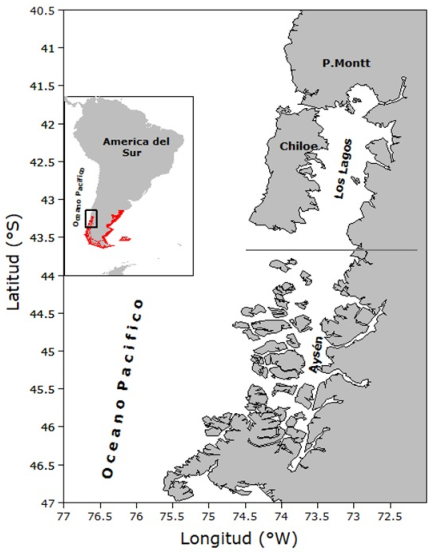
\includegraphics[width=0.6\textwidth]{Figuras/Fig1.pdf}
\caption{Distribución de \textit{S. fuegensis} y diferentes unidades de pesquería (Región de Los Lagos y Aysén).}
\label{Fig1}
\end{figure}

\pagebreak

\hypertarget{unidades-de-stock-y-ecologuxeda}{%
\subsection{2.2. Unidades de stock y
ecología}\label{unidades-de-stock-y-ecologuxeda}}

De acuerdo a Galleguillos \emph{et al}., (2012), a nivel poblacional en
Chile, la sardina austral conforma un único stock genético con una
importante cohesión reproductiva. No obstante, la morfología de
otolitos, fauna parasitaria y tamaño de los individuos, sugieren una
segregación espacial entre los individuos de la Región de Aysén y Los
Lagos, aunque con un nivel de mezcla importante a nivel de los adultos
(26-32\%). Sobre su rol ecológico, está ampliamente documentado que las
especies forrajeras, como sardinas y anchovetas, cumplen un rol clave en
el ecosistema marino, siendo la base alimenticia de mamíferos, aves y
peces de mayor tamaño (Pikitch \emph{et al}., 2012). Diversos
antecedentes concuerdan en destacar a la sardina austral como una
especie clave en el ecosistema de fiordos del sur de Chile, ya que sirve
de base para los otros eslabones de la cadena alimenticia. Neira
\emph{et al}., (2014) indican que sardina austral es presa significativa
de otros recursos pesqueros como merluza austral, merluza de cola y
congrio dorado.

\hypertarget{pesqueruxeda}{%
\subsection{2.3. Pesquería}\label{pesqueruxeda}}

La pesquería se encuentra bajo Régimen Artesanal de Extracción (RAE),
sujeta al establecimiento de cuotas anuales de captura. La captura de
sardina austral es realizada por naves cerqueras, consideradas por la
legislación pesquera de Chile, como artesanales, con máximo de 17,99 m.
de eslora o 100 m\textsuperscript{3} de capacidad de bodega. En la
región de Aysén, la pesquería de sardina austral muestra una actividad
esporádica y de menor intensidad en comparación a la región de Los
Lagos. Desde el año 2012 entre 2 y 10 embarcaciones de cerco operando en
las proximidades de Puerto Chacabuco han declarado desembarque de
sardina austral. En este puerto, se encuentra la pesquera que compra la
totalidad de la materia prima, que tiene como destino la reducción. Se
cuenta con registros oficiales de desembarque a partir del año 2012
(SERNAPESCA, www.sernapesca.cl). Estos, han oscilado en valores promedio
de 5 mil t, entre el año 2012 y 2017. El año 2015 se registró el valor
más alto con 7,5 mil t. El año 2018 en cambio, la actividad fue escaza y
alcanzó un valor mínimo de 652 t. El año 2019, se observó una
recuperación relativa de la actividad pesquera, registrando un valor
oficial de 1352 ton (\textbf{Figura \ref{Fig2}}). \vspace{0.8cm}

\begin{figure}[htb!]
\centering
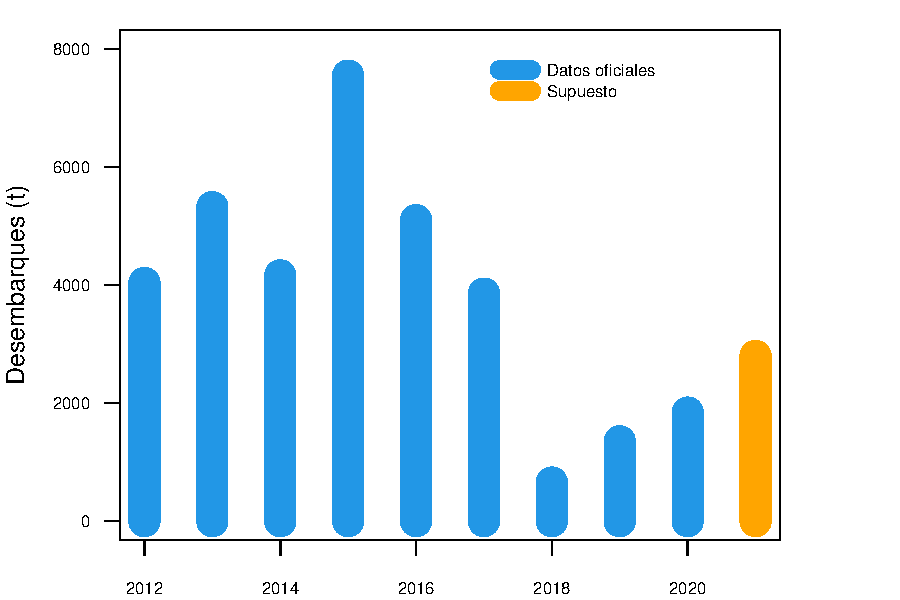
\includegraphics[width=0.8\textwidth]{Figuras/Fig2_InformeFinal-1.pdf}
\caption{Desembarques oficiales anuales de sardina austral en aguas interiores del Mar de Chiloé entre los años 2006 y 2019 (fuente: Sernapesca).}
\label{Fig2}
\end{figure}

\hypertarget{reclutamiento}{%
\subsection{2.4. Reclutamiento}\label{reclutamiento}}

Por ser una actividad esporádica, el monitoreo de la pesquería es
escasa. Se cuenta con unos cuantos muestreos de longitudes que dificulta
caracterizar una dinámica mensual. Se distingue la entrada de individuos
reclutas a partir de abril (\textbf{Figura \ref{Fig3}}). El crucero de
evaluación directa, ha permitido constatar la presencia de ejemplares de
pequeño tamaño presentes en aguas interiores de la Región de Aysén en
los meses de Abril y Mayo (\textbf{Figura \ref{Fig4}}).

\begin{figure}[htb!]
\centering
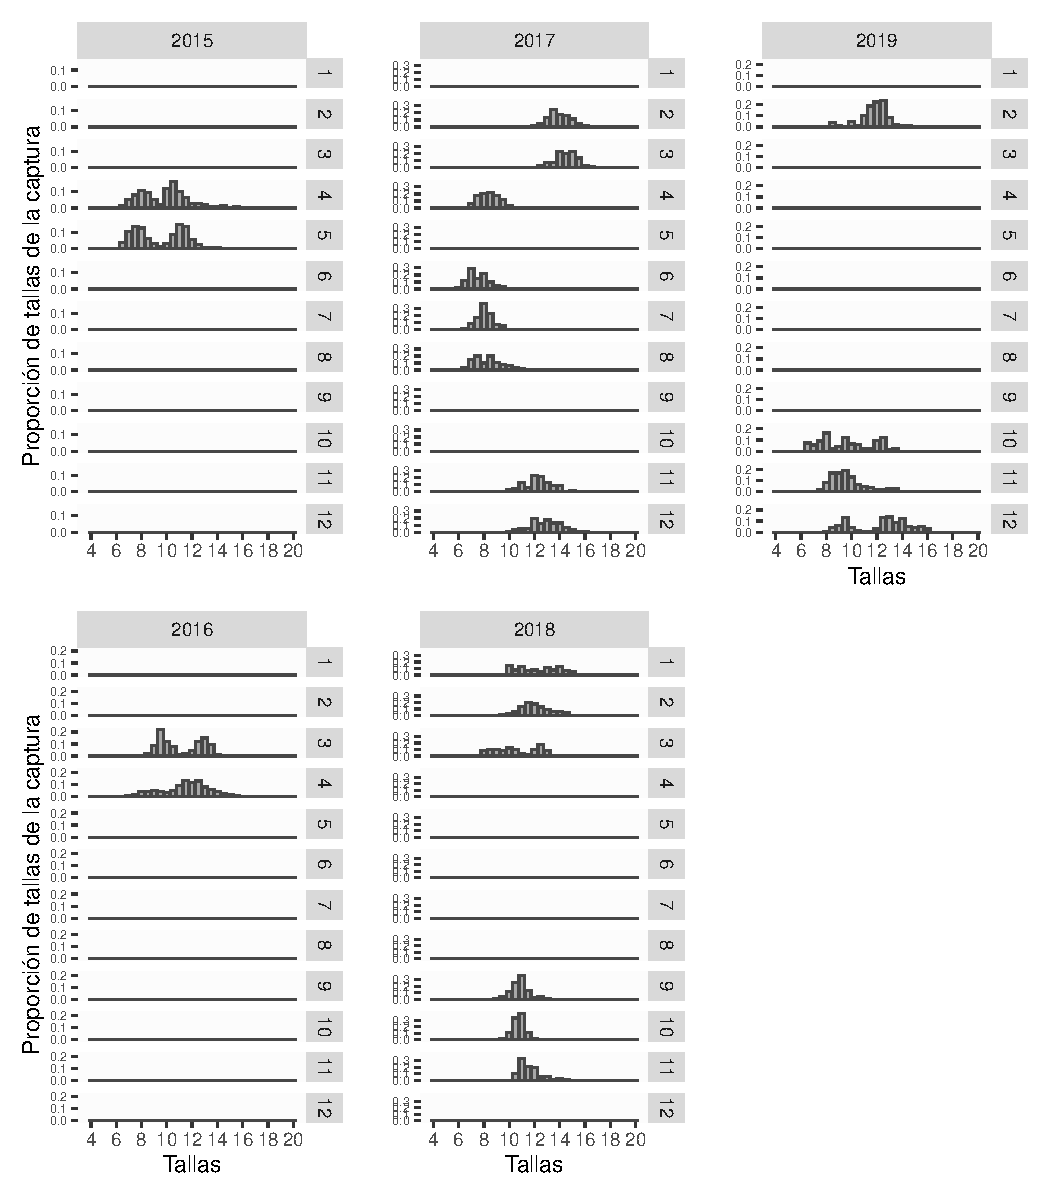
\includegraphics[width=0.8\textwidth]{Figuras/Fig3_InformeFinal-1.pdf}
\caption{ Estructuras de tallas de la flota que opera sobre sardina austral Región de Aysén.}
\label{Fig3}
\end{figure}

\pagebreak

\begin{figure}[htb!]
\centering
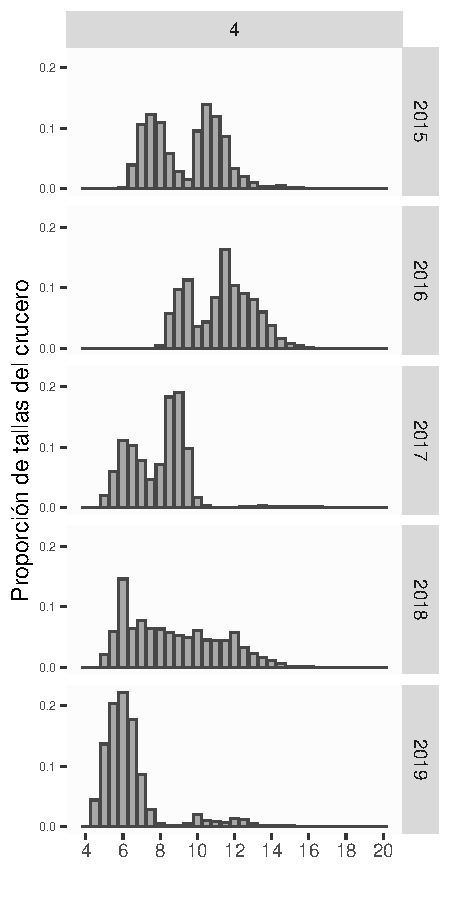
\includegraphics[width=0.8\textwidth]{Figuras/Fig4_InformeFinal-1.pdf}
\caption{Estructuras de tallas obtenidas del crucero acústico  de sardina austral Región de Aysén.}
\label{Fig4}
\end{figure}

\pagebreak

\hypertarget{reproducciuxf3n}{%
\subsection{2.5. Reproducción}\label{reproducciuxf3n}}

Los antecedentes biológicos de la especie provienen principalmente de
estudios realizados en aguas interiores de la Región de Los Lagos. Sobre
su reproducción, Leal \emph{et al}., (2011) señalan que la especie
corresponde a un desovante parcial con una estación reproductiva
concentrada en el segundo semestre (entre septiembre y diciembre) y
donde las hembras desovarían a una longitud media de 13,5 cm LT. Los
mismos autores también discuten que debido a las condiciones del hábitat
de la especie, esta tendría una fecundidad baja, en beneficio de huevos
de mayor tamaño. En la Región de Aysén, Aranís \emph{et al}. (2019),
señalan que las hembras de sardina austral manifestaron en el primer
semestre de 2018 reposo reproductivo y alcanzaron su máxima actividad en
el último trimestre.

\hypertarget{crecimiento-y-mortalidad-natural}{%
\subsection{2.6. Crecimiento y mortalidad
natural}\label{crecimiento-y-mortalidad-natural}}

No existen antecedentes para la Región de Aysén. Sin embrago, para la
Región de Los Lagos, Cerna \emph{et al}., (2007), reportan los
parámetros de crecimiento y mortalidad natural (M) de sardina austral
(\textbf{Tabla \ref{Tab1}}), indicando que la especie presenta un patrón
de crecimiento característicos de los peces pelágicos de pequeño tamaño
como la sardina común y anchoveta. Es catalogada como una especie de
crecimiento rápido y ciclo de vida corto.

\vspace{0.8cm}

\begin{longtable}[]{@{}ll@{}}
\caption{\label{Tab1} Parámetros de crecimiento y mortalidad natural
reportados para sardina austral.}\tabularnewline
\toprule
Parámetro & Cerna \emph{et al}., (2007)\tabularnewline
\midrule
\endfirsthead
\toprule
Parámetro & Cerna \emph{et al}., (2007)\tabularnewline
\midrule
\endhead
\emph{k} & 0,78\tabularnewline
L\textsubscript{inf} & 17,71\tabularnewline
M & 0,83\tabularnewline
\bottomrule
\end{longtable}

\hypertarget{captura-bioluxf3gicamente-aceptable-cba}{%
\subsection{2.7 Captura Biológicamente Aceptable
(CBA)}\label{captura-bioluxf3gicamente-aceptable-cba}}

De acuerdo al ciclo de manejo de esta pesquería, la recomendación de CBA
comienza con el cálculo de la CBA inicial que permite al CCT-PP
establecer el estatus y recomendar el rango de CBA para el año
siguiente. Entre abril y mayo de cada año, el crucero de evaluación
hidroacústico permite estimar la abundancia y biomasa de reclutas
(crucero de verano), esta información junto a los desembarques es
utilizada para actualizar la recomendación inicial de CBA.

El año 2013 se realiza el establecimiento del nuevo Reglamento (D:S: N°
77, Mayo 2013) dispuesto en la Ley General de Pesca y Acuicultura (LGPA)
que establece que las pesquerías deberán alcanzar o mantenerse en torno
del Rendimiento Máximo Sostenido (RMS) considerando las características
biológicas de los recursos explotados. La nueva LGPA establece que el
Comité Científico Técnico será quien recomiende el marco biológico de
referencia, estatus de conservación biológica y rango de CBA.

\pagebreak
\normalsize

\hypertarget{metodologuxeda-de-trabajo}{%
\section{3. METODOLOGÍA DE TRABAJO}\label{metodologuxeda-de-trabajo}}

\hypertarget{objetivo-especuxedfico-1}{%
\subsection{3.1. Objetivo específico
1:}\label{objetivo-especuxedfico-1}}

\vspace{-0.2cm}

\emph{``Implementarprocedimientosdeevaluacióndestockbasadosenprotocoloscientíficosparala
determinación del estatus de los recursos seleccionados con arreglo al
nivel de conocimiento, información e incertidumbre correspondiente,
conforme a los estándares actuales en ciencia pesquera.''}
\vspace{0.5cm}

\hypertarget{modelo-conceptual}{%
\subsubsection{3.1.1. Modelo Conceptual}\label{modelo-conceptual}}

La conceptualización del modelo biológico considera los siguientes
componentes de la dinámica poblacional:

\begin{itemize}
\item
  Estructura geográfica: Se asume que la población de sardina austral en
  la Región de Aysén constituye una unidad de stock. Se asume un stock
  homogéneo al interior de la unidad de pesquería, donde el conjunto de
  individuos está sujeto a la misma probabilidad de crecimiento y
  mortalidad, y donde la migración no es importante.
\item
  Interacción inter-específica: La interacción se asume ocurre en los
  eventos de pesca, de tal manera que el modelo es de tipo
  mono-específico.
\item
  Los desembarques oficiales reportados por Sernapesca corresponden a la
  captura total del recurso en la zona evaluada.
\end{itemize}

La evaluación de stock de sardina austral en la región de Aysén, se
realizó considerando dos aproximaciones para pesquería pobre en datos
(data poor), basadas en el desembarque. Se utilizó en primer lugar el
método de Hilborn \& Mangel (1997) que usa, además de los desembarques,
un índice de abundancia relativo, en este caso la biomasa acústica, para
aproximarse a los cambios en la pendiente de la biomasa del stock en el
tiempo. El método fue usado principalmente para acercarse a algún valor
de depleción (D) del stock para el último año. Este valor de depleción
se utilizó en el segundo método, que define finalmente el estatus del
recurso. El segundo método, corresponde a la aproximación de Zhou
\emph{et al}. (2013), el que utiliza solo las capturas para estimar las
variables de estado como la biomasa y niveles de mortalidad por pesca
(F) que junto a los puntos biológicos de referencia (PBRs) permiten
determinar el estatus y calcular la "Captura Biológicamente Aceptable
(CBA) (\textbf{Figura \ref{Fig5}}). \vspace{0.5cm}

\begin{figure}[htb!]
\centering
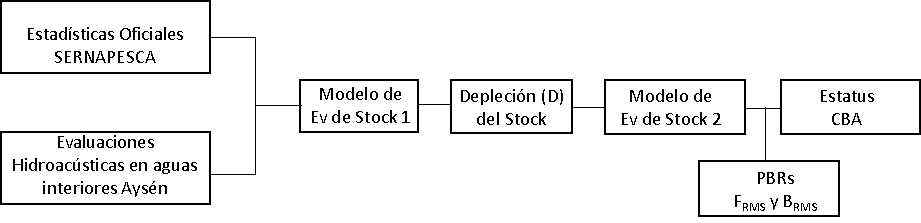
\includegraphics[width=0.8\textwidth]{Figuras/Fig3_ProcEval.pdf}
\caption{Procedimiento de evaluación de stock de sardina austral Región de Aysén.}
\label{Fig5}
\end{figure}

En la implementación del procedimiento de evaluación de stock se
utilizan protocolos científicos basados en la determinación de un
sistema de niveles o ``tiers'' que permiten clasificar la información
disponible de las especies y su pesquería, los cuales se han convertido
en una herramienta de uso común en la asesoría orientada al manejo
pesquero en la actualidad. Para estimar el RMS se utiliza la estrategia
de niveles y de acuerdo con la clasificación del estándar de información
se definen los PBR o ``proxy'' que serán usados para determinar el
estatus del recurso. La definición de los procedimientos de cálculo de
los PBR y del marco de referencia especie específicos se basan en el
estudio ``Revisión de los puntos Biológicos de referencia (Rendimiento
Máximo Sostenible) en las pesquerías nacionales'' (Paya \emph{et al}.,
2014), en cuyo primer taller, se desarrolló en conjunto con expertos
internacionales, un sistema de tres niveles para derivar al \(RMS\)
específico para las pesquerías en Chile. El sistema de clasificación
(Tiers) planteó dos criterios: a) tipo de datos, y b) el método de
evaluación de stock. Los tres tipos de Tiers propuestos para las
pesquerías chilenas, son:

\textbf{Tier 1}: stock para los cuales existe un modelo de evaluación de
stock edad o talla estructurada (e.j. análisis estadístico de captura a
edad) y que suministra estimaciones de la abundancia presente. Dentro de
este Tier, se distinguen dos situaciones comúnmente:

\begin{itemize}
\item
  1a. El punto de referencia máximo rendimiento sostenido (\(RMS\))
  (\(F_{RMS}\) y \(B_{RMS}\)) y el punto de referencia \(B_{LIM}\)
  pueden ser estimados con confiabilidad (u otro especificado) desde los
  parámetros estimados dentro de los modelos de evaluación.
\item
  1b. Proxies para los puntos de referencia en 1a son escogidos. La
  selección de estos proxies debería tomar en cuenta la incertidumbre
  del modelo de evaluación y el grado de resiliencia (o la falta de
  ella) de la especie.
\end{itemize}

\textbf{Tier 2}: stock para los cuales existe un modelo de biomasa
dinámica (también conocidos como modelo de producción) o una
aproximación empírica basada en datos de captura o abundancia relativa.
Otros datos relevantes pueden también ser usados.

\textbf{Tier 3}: stock para los cuales no hay datos suficientes que
permitan la aplicación de un modelo dinámico. Aproximaciones empíricas
basadas inicialmente en datos de captura (sin datos de abundancia
relativa), parámetros de historia de vida, y/o evaluaciones directas han
sido usadas.

En el caso particular de sardina austral en la Región de Aysén, por el
momento, no existe información suficiente para desarrollar un modelo
estructurado a la edad o talla y realizar estimaciones confiables de
rendimiento máximo sostenido (\(RMS\)). Hasta la fecha se cuenta con
información de los desembarques y un índice de abundancia relativo
proveniente de los cruceros de evaluación directa. Estos antecedentes
permiten clasificar a sardina austral Región de Aysén en el Tier 2
(\textbf{Figura \ref{Fig6}}).

\vspace{0.5cm}

\begin{figure}[htb!]
\centering
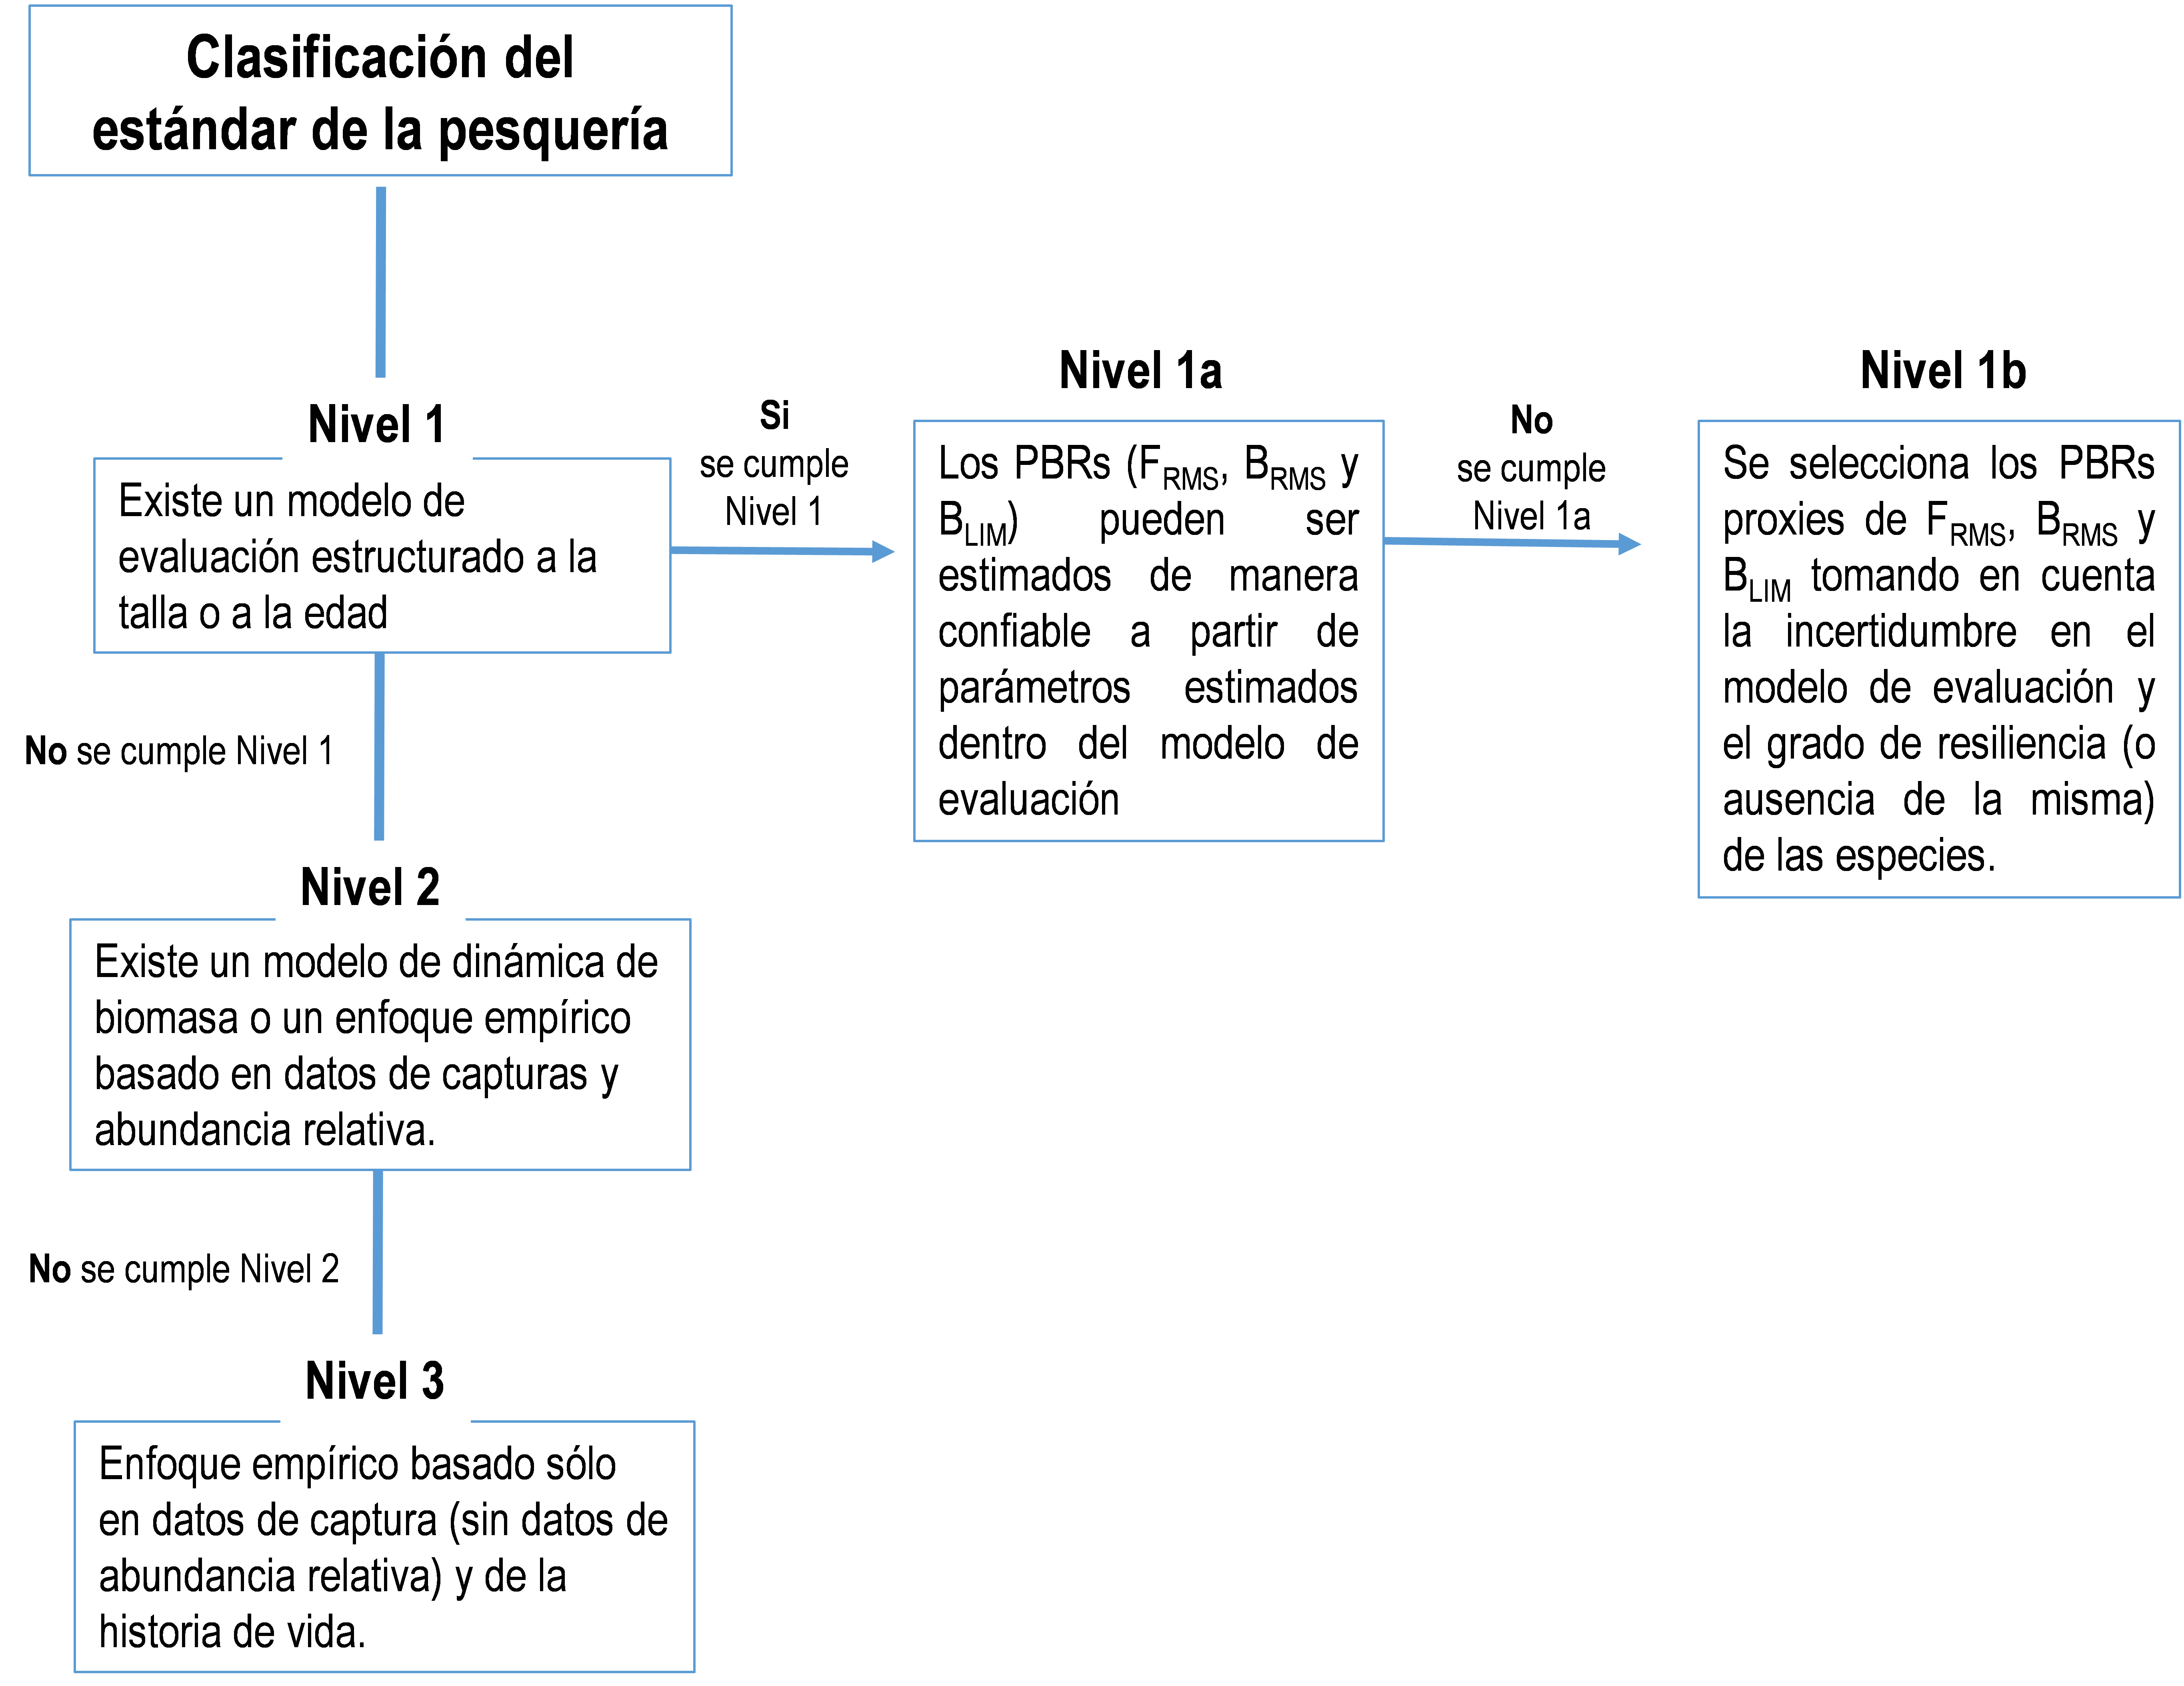
\includegraphics[width=0.7\textwidth]{Figuras/Fig7_InformeFinal.png}
\caption{Sistema de niveles para la determinación de los PBRs de acuerdo a la cantidad, tipo y la calidad de la información disponible y, métodos de evaluación de stock empleados en cada pesquería.}
\label{Fig6}
\end{figure}

\hypertarget{datos-de-entrada-al-modelo-de-evaluaciuxf3n-de-stock}{%
\subsubsection{3.1.2. Datos de entrada al modelo de evaluación de
stock}\label{datos-de-entrada-al-modelo-de-evaluaciuxf3n-de-stock}}

A continuación, se detalla y fundamenta el conjunto de datos a emplear
en la evaluación de stock de sardina austral en aguas interiores de la
Región de Aysén. Se utiliza información del desembarque total anual de
la especie en la Región de Aysén, proporcionada por el Servicio nacional
de pesca (Sernapesca). Utiliza también información las evaluaciones
directas (2006, 2008, 2011, 2013-2019) del recurso en la zona del mar
interior de Aysén.

\hypertarget{desembarques}{%
\paragraph{Desembarques:}\label{desembarques}}

\quad

Corresponde a la extracción registrada en puerto, independiente de la
zona de procedencia. Tiene valor en definir la importancia relativa de
los distintos puertos de descarga, por lo tanto, es de mayor interés
administrativo y/o comercial de la actividad. Su propósito es
cuantificar los volúmenes totales y por especie, que efectivamente se
reciben en la descarga o desembarque. Las estadísticas oficiales de los
desembarques son sistematizadas por Sernapesca, sobre una base mensual,
por tipo de flota, puerto de desembarque y especie objetivo. Cabe
señalar que en la pesquería pelágica el concepto de captura es igual al
del desembarque. Para la evaluación de stock de sardina austral en aguas
interiores de la Región de Aysén la serie se inicia el año 2012.

\hypertarget{sub-reporte}{%
\paragraph{Sub-reporte:}\label{sub-reporte}}

\quad

La pesquería, aunque dominada por sardina austral, es de carácter mixta,
apareciendo en ocasiones junto a sardina común y anchoveta. La
restricción por cuotas para sardina austral, puede motivar a los
usuarios a reportar una especie por otra. Otro antecedente, es la escaza
presencia de certificadores en aguas interiores.

\hypertarget{descarte}{%
\paragraph{Descarte:}\label{descarte}}

\quad

La pesquería de sardina austral en aguas interiores es efectuada por una
flota artesanal de cerco, que destina la captura principalmente a la
reducción, por lo tanto, tendrían bajas tasas de descarte. En la
actualidad, los estudios sobre descarte se concentran en la región de
Los Lagos y fue incorporada al programa de observadores científicos a
partir del año 2017 (Vega \emph{et al}., 2020).

\hypertarget{seguimiento-de-la-pesqueruxeda}{%
\paragraph{Seguimiento de la
pesquería:}\label{seguimiento-de-la-pesqueruxeda}}

\quad

El monitoreo de la pesquería de sardina austral en la Región de es
reciente y es realizado por el Proyecto de Investigación Situación
Pesquerías de Peces Pelágicos, que forma parte del Programa de
Seguimiento de las Principales Pesquerías Nacionales y es encargado por
la Subsecretaría de Pesca a IFOP. Debido a la baja frecuencia de
operación de las embarcaciones, el monitoreo es complejo y se cuenta con
escasa información de la actividad pesquera. Esto no permite aun
construir un modelo de evaluación de stock más complejo.

\hypertarget{cruceros-de-evaluaciuxf3n-hidroacuxfastica}{%
\paragraph{Cruceros de evaluación
hidroacústica:}\label{cruceros-de-evaluaciuxf3n-hidroacuxfastica}}

\quad

A partir del año 2013 se han realizado en la zona del mar interior de
Aysén, 7 cruceros de evaluación directa, donde se estima la biomasa y
estructura de longitudes de peces pelágicos y en particular de sardina
austral. El último estudio fue realizado en abril/mayo de 2019 y es
utilizado para estimar el estatus y CBA de sardina austral.

\vspace{0.9cm}

\hypertarget{paruxe1metros-de-historia-de-vida}{%
\paragraph{Parámetros de historia de
vida:}\label{paruxe1metros-de-historia-de-vida}}

\quad

Los procedimientos de evaluación de stock, recogen el conocimiento de
otros estudios que reportan información asociada a los parámetros del
ciclo vital de la especie, como la mortalidad natural (M), el
crecimiento y madurez. Sin embrago, en este caso no se cuenta con
estudios específicos sobre los parámetros biológicos de la especie en la
Región de Aysén. Toda la información disponible en Chile procede de los
estudios realizados en la zona del mar interior de Chiloé.

\hypertarget{evaluaciuxf3n-de-stock}{%
\subsubsection{3.1.3. Evaluación de
stock}\label{evaluaciuxf3n-de-stock}}

La metodología empleada en el desarrollo del proyecto está basada en el
enfoque de procesos y sistemas, entendiendo los objetivos de éste como
los componentes de un sistema de información y conocimiento. Además, el
enfoque metodológico se sustenta en la aplicación del método científico
y los análisis se basan en el uso de la mejor información y conocimiento
disponibles, consecuente con la aplicación del enfoque precautorio para
la pesca (FAO, 1996). En este contexto, se implementa un proceso de
evaluación de stock que considera las siguientes etapas:

\vspace{0.5cm}

\textbf{a) Análisis y procesos preliminares}: En esta etapa se recopilan
los antecedentes y datos de la pesquería y del recurso, en conjunto con
la estimación de indicadores de abundancia relativa y otras piezas de
información, como los parámetros de crecimiento y mortalidad natural. Se
realiza un análisis crítico de los datos e información disponibles y
finalmente se determina el Estándar Metodológico para la Evaluación
(EME).

\textbf{b) Especificación del modelo de evaluación de stock}: Se define
el modelo de evaluación de stock, que incluye la definición de
supuestos, hipótesis, condiciones iniciales de la dinámica del stock,
definición de los modelos de los procesos (dinámica), de las
observaciones y penalizaciones. La formulación estadística del modelo se
presenta en las secciones siguientes.

\textbf{c) Inferencia estadística}: Una vez definido el modelo de
dinámica y los datos de entrada, se procede a la estimación de los
parámetros y estados no observables, utilizando un enfoque de
probabilidad frecuentista.

\textbf{d) Análisis, estatus y diagnóstico}: Luego de ajustado el modelo
de evaluación de stock y obtenidas las distribuciones posteriores de los
parámetros, se estiman los puntos biológicos de referencia, se analizan
las variables de estado y flujo, se construye el diagrama de fases de
explotación y finalmente se determina el estatus del recurso.

\textbf{e) Análisis prospectivos}: Con el propósito de determinar los
niveles de explotación que aseguran la sustentabilidad del recurso, se
proyecta el stock en el mediano plazo, bajo un conjunto de tácticas y
estrategias de explotación, evaluándose las probabilidades (riesgo) de
no cumplir con los objetivos de administración.

\textbf{f) Conclusiones y recomendaciones}: Una vez concluidas las
etapas anteriores, se procede a sintetizar las principales brechas del
conocimiento y limitaciones, tanto de parámetros del ciclo vital de la
especie, como de datos de la pesquería. Además, se realiza un análisis
crítico del modelo de evaluación de stock, junto con los resultados
obtenidos, para finalmente elaborar el programa de mejoramiento continuo
de la calidad de la asesoría científica.

\vspace{0.8cm}

\hypertarget{descripciuxf3n-del-modelo-base}{%
\paragraph{Descripción del modelo
base}\label{descripciuxf3n-del-modelo-base}}

\quad

La evaluación cubrirá el período 2012-2020 y se realiza considerando
métodos basado en la captura. La información disponible para estimar los
niveles de biomasa para sardina austral en la región de Aysén
corresponde, según el método de Hilborn \& Mangel (1997), a los
desembarques totales anuales entre a partir del 2013. Se utiliza
también, el índice de abundancia relativa de biomasa, estimada por el
crucero de evaluación directa en el mar interior de la región de Aysén.
El método de Zhou \emph{et al}. (2013) en tanto, utiliza únicamente los
desembarques observados en la zona desde el año 2012 y un valor de
depleción máximo (D) derivado del primer método. Se utiliza también un
nivel supuesto de desembarque del año 2020 correspondiente al valor de
CBA establecido por el CCT-PP. La información empleada, se resume en la
\textbf{Tabla \ref{Tab2}}. Es importante señalar que este tipo de
métodos suponen que las capturas del recurso son verdaderas y que éste,
constituye un stock cerrado en el área de estudio. Es decir, no hay
inmigración o emigración. A pesar de dichas limitaciones, esta
aproximación es utilizada para estimar los Puntos Biológicos de
Referencia (PBR), estatus y cálculo de CBA.

\begin{longtable}[]{@{}ccc@{}}
\caption{\label{Tab2} Información utilizada en la evaluación de stock de
sardina austral en la Región de Aysén.}\tabularnewline
\toprule
Año & Captura (t) & Índice Acústico\tabularnewline
\midrule
\endfirsthead
\toprule
Año & Captura (t) & Índice Acústico\tabularnewline
\midrule
\endhead
2012 & 4033 &\tabularnewline
2013 & 5318 & 106685\tabularnewline
2014 & 4163 & 32841\tabularnewline
2015 & 7547 & 21973\tabularnewline
2016 & 5097 & 44923\tabularnewline
2017 & 3853 & 35346\tabularnewline
2018 & 653 & 24805\tabularnewline
2019 & 1352 & 6568\tabularnewline
2020 & 1839 & -\tabularnewline
2021 & 2797* & 58922\tabularnewline
\bottomrule
\end{longtable}

\begin{itemize}
\tightlist
\item
  *Captura 2021 = CBA establecida para el año en curso por el CCTPP.
\end{itemize}

\hypertarget{marco-teuxf3rico}{%
\paragraph{Marco Teórico}\label{marco-teuxf3rico}}

\quad

Varias clases de modelos se utilizan para la evaluación de stock, en la
presente investigación se adopta un modelo de producción que permite
estudiar la evolución de la Biomasa total del stock en su globalidad,
contemplando entre otros efectos, la tendencia de la biomasa obtenida
por el crucero de evaluación directa. Dicho modelo no considera la
estructura de edades o de tallas del stock, las cuales dan lugar a la
aplicación de los denominados modelos estructurados.

\hypertarget{modelo-de-schaefer}{%
\paragraph{Modelo de Schaefer}\label{modelo-de-schaefer}}

\quad

Este modelo desarrollado por Schaefer (1954) toma como base el modelo de
crecimiento logístico de población desarrollado por Verhulst (1838).
Usualmente en la literatura pesquera se conoce como un ``modelo de
producción excedentaria''. Dicho modelo es la base de las metodologías
(Hilborn \& Mangel 1997; Zhou \emph{et al}. 2013) aplicadas para evaluar
la pesquería de sardina austral en la Región de Aysén. El modelo de
Schaefer se describe de la siguiente manera:

\vspace{0.5cm}
\begin{equation}
B_{t+1}=B_t + rB_t \left({1+\displaystyle\frac{B_t}{K}}\right)-C_t
\end{equation} 
\vspace{0.5cm}

\(B_t\) es la biomasa al tiempo \(t\), En este modelo la tasa intrínseca
de crecimiento r y la capacidad de carga \(K\) son constantes en el
tiempo.

\hypertarget{muxe9todo-de-hilborn-mangel-1997}{%
\paragraph{Método de Hilborn \& Mangel
(1997)}\label{muxe9todo-de-hilborn-mangel-1997}}

\quad

En la aproximación de Hilborn \& Mangel (1997) un índice (\(I_t\)) de
abundancia como la Captura por Unidad de Esfuerzo (CPUE) o estimaciones
provenientes de un crucero, pueden ser usados para calibrar el modelo y
estimar la biomasa del stock incorporando incertidumbre. De esta manera,
de acuerdo a los autores, las estimaciones de los parámetros son más
eficientes. El error que se incorpora en este análisis proviene de
observación en el índice acústico (\(I_t\)) y para desarrollar este
modelo, uno de los supuestos básicos es la proporcionalidad entre dicho
índice y la Biomasa (\(B\)) del stock:

\vspace{0.5cm}
\begin{equation}
I_t=q*B_t
\end{equation} 
\vspace{0.5cm}

En este caso \(q\) es el coeficiente de capturabilidad del crucero de
evaluación directa.

Una vez obtenido el índice de abundancia, se compara con el índice
observado para tener una medida del desempeño del modelo, es decir, se
calcula el error (\(e\)) de la siguiente manera:

\vspace{0.5cm}
\begin{equation}
\sigma_{obs}=\sqrt{\frac{1}{n-1}\sum_{t-1}^{n}\left(ln(I_{t obs})/ln( _{t esp})\right)^2}
\end{equation} 
\vspace{0.5cm}

Se empleó el ajuste mediante la verosimilitud con un estimador de error
con varianza constante (\(\varepsilon=N(0,\sigma^2\)) debido a que este
método brinda los mejores resultados (Chen y Andrews, 1998; Williams y
Prager, 2002). Una vez encontrado los valores de \(r\) y \(K\) que
minimizan la función objetivo (\(L\)), se calcula la serie de Biomasas
predicha por modelo y la observada.

\vspace{0.5cm}
\begin{equation}
L(\theta|r,k)=\frac{1}{2}*ln(\sigma^2)+\left(\frac{(ln(I_{t obs})/ln(I_{t esp}))^2}{2 \sigma^2} \right)
\end{equation} 
\vspace{0.5cm}

Esta metodología es usada como una forma de acercarse a un valor de
depleción (\(D\)) del stock, cuyo valor es usado como input en la
metodología de Zhou \emph{et al}. (2013), la cual define el estatus y
estima la CBA del recurso para el año siguiente en el hito 1 y el año
actual en el hito 2.

\hypertarget{muxe9todo-de-zhou-et-al.-2013}{%
\paragraph{\texorpdfstring{Método de Zhou \emph{et al}.
(2013)}{Método de Zhou et al. (2013)}}\label{muxe9todo-de-zhou-et-al.-2013}}

\quad

Este método también consiste en estimar los parámetros \(r\) y \(K\) del
modelo de Schaefer. El método en vez de asignar priors con límites,
utiliza priors sin restricciones para \(K\) y \(r\), según,
\(0 < K < \infty\), y \(0 < r < \infty\) (hay que tener en cuenta que
\(K\) y \(r\) están correlacionados negativamente así que en cierta
forma existe una restricción). Sin embargo, pueden definirse ciertos
límites razonables para \(r\) y \(K\). Por ejemplo, para \(K\) pueden
usarse valores entre 10 y \(100*C_{max}\) (\(C_{max}\)) es la captura
máxima en la serie de tiempo), y \(r\) entre 0 y 3. Además se debe
suponer una serie de niveles de agotamiento o depleción (\(D\))
\(D=Be/K\), \(D=0,05\) y \(D=0,95\). \(Be\) se asume como la biomasa
verdadera al final del periodo. Si \(d=1\), significa \(Be=K\), lo cual
es generalmente imposible cuando la captura es mayor que 0 en los
últimos años. A pesar de que la evaluación se puede llevar a cabo sin
conocer los límites superiores de \(r\) y \(K\), el método también puede
utilizar otra información como los parámetros de historia de vida para
obtener aproximaciones de \(r\) y \(K\) (Zhou \emph{et al}., 2012). La
hipotesis básica para el nivel de agotamiento supuesto, proviene del
primer método.

Estos valores de \(K\) y \(r\) junto con las capturas conocidas son
usados para realizar simulaciones estocásticas utilizando el modelo de
biomasa de Graham-Schaefer sin restricciones en otras variables. En cada
iteración se toma aleatoriamente un valor de \(r\) y \(K\) desde una
distribución uniforme del rango de valores estimados de \(r\) y \(K\).
Un número grande de simulaciones (e.j. 1000) tanto de trayectorias de
las biomasas, así como biomasas finales, y niveles de agotamiento son
almacenados. Una selección de simulaciones es seleccionada normalmente
aquella donde no se cumpla la condición \(B_t\leq 0\). Cuando los
valores más probables de \(K\) y \(r\) son identificados, los puntos
biológicos de referencia de RMS, \(B_{RMS}\) y \(F_{RMS}\) junto a los
niveles de \(D\) pueden ser derivados.

\hypertarget{informaciuxf3n-y-paruxe1metros-de-entrada}{%
\paragraph{Información y parámetros de
entrada}\label{informaciuxf3n-y-paruxe1metros-de-entrada}}

\quad

La información utilizada para estimar los niveles de biomasa para
sardina austral en la Región de Aysén utilizando el método de Zhou
\emph{et al}. (2013) para datos pobres, corresponde a los desembarques
oficiales entre 2012 -- 2020 y un supuesto de captura durante el año
2021. La prior para la tasa de crecimiento poblacional, \(r\), fue
definida utilizando la aproximación de Zhou \emph{et al}. (2012) quien
hace uso de la mortalidad natural (\(M\)) para estimar los valores para
la prior de \(r\). Estos autores definen la relación entre \(F_{RMS}\) y
\(M\) equivalente a \(F_{RMS} = 0,87M\) para el caso de peces
teleósteos. A su vez, de los modelos de producción se tiene que
\(r=2F_{RMS}\) (Haddon, 2001). De esta forma, \(r\), puede expresarse
como una función de la mortalida natural, \(M\), según \(r = 2*0,87M\)

Como valores para la prior de \(K\) se utilizó el criterio de la captura
máxima observada como límite inferior, y una amplificación por 50, como
límite superior de \(K\), esto es de 7547 ton a 377350 toneladas
respectivamente. Como intervalo para los valores de la reducción del
stock, se tomaron valores entre 0,10 a 0,80 a intervalos de 0,05.

En la \textbf{Tabla \ref{Tab3}}, se presenta un resumen del acercamiento
metodológico que es empleado para la evaluación de stock en la pesquería
de sardina austral en la Región de Aysén a través la aproximación de
método de Zhou \emph{et al}. (2013).

\vspace{0.8cm}

\begin{longtable}[]{@{}ll@{}}
\caption{\label{Tab3} Resumen de la metodología propuesta para la
evaluación de stock de sardina austral en la Región de
Aysén.}\tabularnewline
\toprule
\begin{minipage}[b]{0.30\columnwidth}\raggedright
Recurso Objetivo\strut
\end{minipage} & \begin{minipage}[b]{0.64\columnwidth}\raggedright
Sardina austral Aysén\strut
\end{minipage}\tabularnewline
\midrule
\endfirsthead
\toprule
\begin{minipage}[b]{0.30\columnwidth}\raggedright
Recurso Objetivo\strut
\end{minipage} & \begin{minipage}[b]{0.64\columnwidth}\raggedright
Sardina austral Aysén\strut
\end{minipage}\tabularnewline
\midrule
\endhead
\begin{minipage}[t]{0.30\columnwidth}\raggedright
Área geográfica\strut
\end{minipage} & \begin{minipage}[t]{0.64\columnwidth}\raggedright
Aguas interiores Región de Aysén\strut
\end{minipage}\tabularnewline
\begin{minipage}[t]{0.30\columnwidth}\raggedright
Período de análisis\strut
\end{minipage} & \begin{minipage}[t]{0.64\columnwidth}\raggedright
2012-2020\strut
\end{minipage}\tabularnewline
\begin{minipage}[t]{0.30\columnwidth}\raggedright
Información a emplear\strut
\end{minipage} & \begin{minipage}[t]{0.64\columnwidth}\raggedright
Desembarque oficial en la Región\strut
\end{minipage}\tabularnewline
\begin{minipage}[t]{0.30\columnwidth}\raggedright
Modelos a emplear\strut
\end{minipage} & \begin{minipage}[t]{0.64\columnwidth}\raggedright
Modelo de datos pobre orientado a la posteriori\strut
\end{minipage}\tabularnewline
\begin{minipage}[t]{0.30\columnwidth}\raggedright
Referencia\strut
\end{minipage} & \begin{minipage}[t]{0.64\columnwidth}\raggedright
Zhou \emph{et al}. (2013)\strut
\end{minipage}\tabularnewline
\begin{minipage}[t]{0.30\columnwidth}\raggedright
Uso de ponderadores de información\strut
\end{minipage} & \begin{minipage}[t]{0.64\columnwidth}\raggedright
Coeficientes de variación fijos\strut
\end{minipage}\tabularnewline
\begin{minipage}[t]{0.30\columnwidth}\raggedright
Plataforma de programación\strut
\end{minipage} & \begin{minipage}[t]{0.64\columnwidth}\raggedright
R\strut
\end{minipage}\tabularnewline
\begin{minipage}[t]{0.30\columnwidth}\raggedright
Incertidumbre de variables y parámetros\strut
\end{minipage} & \begin{minipage}[t]{0.64\columnwidth}\raggedright
Simulaciones estocásticas\strut
\end{minipage}\tabularnewline
\begin{minipage}[t]{0.30\columnwidth}\raggedright
Estimación de PBR\strut
\end{minipage} & \begin{minipage}[t]{0.64\columnwidth}\raggedright
Modelo de producción de Schaefer\strut
\end{minipage}\tabularnewline
\begin{minipage}[t]{0.30\columnwidth}\raggedright
Desempeño de modelos\strut
\end{minipage} & \begin{minipage}[t]{0.64\columnwidth}\raggedright
Análisis de sensibilidad de supuestos\strut
\end{minipage}\tabularnewline
\begin{minipage}[t]{0.30\columnwidth}\raggedright
Estatus del recurso\strut
\end{minipage} & \begin{minipage}[t]{0.64\columnwidth}\raggedright
Diagrama de fases entre la biomasa total (BT) vs la mortalidad por pesca
(F) relativas\strut
\end{minipage}\tabularnewline
\begin{minipage}[t]{0.30\columnwidth}\raggedright
Simulación de táctica de captura\strut
\end{minipage} & \begin{minipage}[t]{0.64\columnwidth}\raggedright
F constante basada en PBR\strut
\end{minipage}\tabularnewline
\begin{minipage}[t]{0.30\columnwidth}\raggedright
Horizonte de proyección\strut
\end{minipage} & \begin{minipage}[t]{0.64\columnwidth}\raggedright
1 a 5 años\strut
\end{minipage}\tabularnewline
\begin{minipage}[t]{0.30\columnwidth}\raggedright
Fuente de error de proyección\strut
\end{minipage} & \begin{minipage}[t]{0.64\columnwidth}\raggedright
error de parámetros y error de proceso\strut
\end{minipage}\tabularnewline
\bottomrule
\end{longtable}

\pagebreak

\hypertarget{objetivo-especuxedfico-2}{%
\subsection{3.2. Objetivo específico
2:}\label{objetivo-especuxedfico-2}}

\vspace{-0.2cm}

\emph{``Establecer el estatus actualizado de estos recursos, sobre la
base de sus principales indicadores estandarizados de estado y flujo,
incorporando, cuantificando y propagando la incertidumbre subyacente a
la pesquería.''} \vspace{0.5cm}

\hypertarget{estatus}{%
\subsubsection{3.2.1. Estatus}\label{estatus}}

\vspace{0.8cm}

\hypertarget{variables-poblacionales}{%
\paragraph{Variables Poblacionales}\label{variables-poblacionales}}

\quad

Se analiza la variabilidad en las tendencias poblacionales de la Biomasa
total (BT) y Mortalidad por pesca (F) del stock durante el periodo de
tiempo considerado en la evaluación.

\hypertarget{indicadores-del-estado-del-stock}{%
\paragraph{Indicadores del estado del
stock}\label{indicadores-del-estado-del-stock}}

\quad

El estado del recurso se establece en base a la posición relativa de la
biomasa desovante y mortalidad por pesca relacionada a la explotación
pesquera v/s Puntos Biológicos de Referencia (PBR) basados en el
Rendimiento Máximo Sostenido (RMS). En el contexto de la Ley General de
Pesca y Acuicultura (LGPA) se establece que las pesquerías deberán
alcanzar o mantenerse en torno del RMS considerando las características
biológicas de los recursos explotados. El RMS se produce cuando el stock
desovante se reduce notablemente antes que el reclutamiento se vea
impactado, en promedio, para lo cual exige, se estimen los siguientes
PBRs:

• Biomasa desovante en el Rendimiento Máximo Sostenible (\(BD_{RMS}\)),
bajo la cual el recurso califica en sobre-explotación.

• Mortalidad por Pesca en el Rendimiento Máximo Sostenible
(\(F_{RMS}\)), sobre la cual el recurso califica en sobre-explotación.

• Biomasa desovante límite (\(B_{LIM}\)) bajo la cual una pesquería
califica de agotada o colapsada.

• Mortalidad por Pesca límite (\(F_{LIM}\)) a partir de la cual el
recurso califica en sobrepesca.

\vspace{0.8cm}

Este estudio se basa en el Marco Biológico de Referencia establecido por
el Comité Científico Técnico- Pesquerías de Pequeños Pelágicos (CCT-PP)
en base a los avances realizados durante el 2013 y 2014 en la
determinación de Puntos Biológicos de Referencia (PBR) y del Rendimiento
Máximo Sostenido (RMS) del proyecto ``Revisión y estimación de los PBR
(Rendimiento Máximo Sostenido) para las principales pesquerías
nacionales'' (Payá \emph{et al}., 2014). Al respecto, el reporte propone
usar como objetivo, el nivel de mortalidad por pesca que reduce hasta un
55\% (F55) la biomasa desovante virginal (\(55\%BD_0\)). Tal nivel de
reducción corresponde a un 60\% en la Biomasa desovante por recluta
(\(60\%BDPR0\)). Este PBR coincide con el valor propuesto como objetivo
en este recurso hasta el reporte previo.

Se enfatiza en el hecho que la \(F_{RMS}\) es el punto de referencia de
biomasa desovante, que en general, será una aproximación más que
provenir de un cálculo formal. Las elecciones específicas para los
stocks pueden depender del nivel de incertidumbre, del valor asignado en
los servicios de los ecosistemas y del nivel de riesgo que los
administradores y la sociedad deseen asumir (Payá \emph{et al}., 2014).

\hypertarget{puntos-bioluxf3gicos-de-referencia}{%
\paragraph{Puntos Biológicos de
Referencia}\label{puntos-bioluxf3gicos-de-referencia}}

\quad

Los puntos biológicos de referencia (PBR) de sardina austral en la
Región de Aysén, fueron calculados en base al método basado en las
capturas (Zhou \emph{et al}. 2013) y utilizando el modelo de excedentes
productivos de Schaefer (1954). Así, la biomasa del rendimiento máximo
sostenido (RMS) en el modelo de Schaefer corresponde a \(B_{RMS}=K/2\),
donde \(B_{RMS}\) indica la biomasa del RMS y K corresponde a la
capacidad de carga. La mortalidad por pesca de RMS (\(F_{RMS}\)) se
obtiene según \(F_{RMS}=r/2\), donde r corresponde a la tasa de
crecimiento poblacional. La biomasa límite (\(B_{LIM}\)) se alcanza a la
mitad \(B_{RMS}\), y por lo tanto \(B_{lím}= B_{RMS}/2\). El RMS se
define como \(RMS=Kr/4\) (\textbf{Tabla \ref{Tab4}}).

\vspace{0.8cm}

\begin{longtable}[]{@{}cccc@{}}
\caption{\label{Tab4} Puntos de Referencia objetivo y límites para
sardina austral que definen su estado y criterio de
explotación.}\tabularnewline
\toprule
RECURSO & \(F_{RMS}\) proxy & \(B_{RMS}\) proxy &
\(B_{LIM}\)\tabularnewline
\midrule
\endfirsthead
\toprule
RECURSO & \(F_{RMS}\) proxy & \(B_{RMS}\) proxy &
\(B_{LIM}\)\tabularnewline
\midrule
\endhead
Sardina austral Región de Aysén & \(F_{RMS} = r/2\) & \(B_{RMS}=K/2\) &
\(B_{RMS}/2\)\tabularnewline
\bottomrule
\end{longtable}

\vspace{0.5cm}

\hypertarget{diagrama-de-fases-de-explotaciuxf3n}{%
\paragraph{Diagrama de fases de
explotación}\label{diagrama-de-fases-de-explotaciuxf3n}}

\quad

El estado del recurso se estableció en base a la posición relativa de la
mortalidad por pesca y biomasa desovante versus los puntos biológicos de
referencia basado en el rendimiento máximo sostenible (RMS), tales como,
\(F_{RMS}\) y \(BD_{RMS}\). De este modo se obtienen los indicadores del
estatus (\(F/F_{RMS}\) y \(BD/BD_{RMS}\)) que permiten construir un
diagrama de fase, donde los puntos de referencia biológicos se muestran
en las líneas verticales y horizontales en 1. Las líneas verticales
indican la biomasa desovante en el rendimiento máximo sostenible
(\(BD_{RMS}\)), bajo el cual el recurso califica en sobre- explotación y
biomasa desovante límite (\(BD_{LIM}\)) bajo el cual una pesquería
califica de agotada y/o colapsada y la línea horizontal el punto de
referencia correspondiente a la mortalidad por pesca en el rendimiento
máximo sostenible (\(F_{RMS}\)), sobre la cual el recurso califica en
sobre-explotación. La \textbf{Figura \ref{Fig8}} muestra el diagrama de
fase definido por el CCT-PP para las pesquerías de pelágicos pequeños.
El estado de la pesquería en Plena Explotación se define en la Ley de
Pesca como ``un nivel en el que el punto biológico ha alcanzado o está a
su máximo rendimiento sostenido''. Debido a la variabilidad natural en
las condiciones ecológicas y ambientales, Frms no es estática, pero
fluctuará alrededor de \(BD_{RMS}\). Adicionalmente, el CCT\_PP
incorporó el concepto de sobrepesca, precisando algunas definiciones y
se pronunció respecto a la zona de plena explotación, según consta en
acta número 5 (11 al 14 de noviembre de 2014). Los aspectos más
relevantes son los que a continuación se describen:

\vspace{0.5cm}

\textbf{Sobrepesca}: Este Comité consideró necesario diferenciar al
interior de la zona de sobreexplotación definida por la LGPA, el área de
sobrepesca, con el objeto de aplicar las medidas de Administración más
acordes con dicha condición. En tal sentido, la sobrepesca ocurriría
cuando la mortalidad por pesca F (variable de flujo y de control) exceda
un valor considerado umbral o límite que en este caso, corresponde al
valor superior, en mortalidad por pesca (valor relativo al objetivo), de
la zona de plena explotación.

\textbf{Sobreexplotado}: En correspondencia con la definición anterior,
la sobreexplotación ocurriría cuando la biomasa (variable de estado) cae
bajo un valor umbral o límite, correspondiendo éste al valor inferior en
biomasa (valor relativo al objetivo) de la zona de plena explotación.

\textbf{Rango de Plena Explotación}: El CCT-PP recomendó por consenso
los siguientes rangos que definen la condición de Plena Explotación de
los recursos pelágicos, considerando los siguientes límites en biomasa y
el correspondiente par ordenado en mortalidad por pesca:

\vspace{0.5cm}

\begin{itemize}
\item
  Límite bajo el objetivo de manejo = 10\% Bajo \(BD_{RMS}\): Este
  criterio tiene como propósito el establecimiento de una banda estrecha
  en torno al RMS, que genere un área no deseada pequeña que en lo
  posible sea menor o igual al área de incertidumbre total del sistema,
  donde la biomasa está bajo la biomasa objetivo y a su vez, la
  mortalidad por pesca es mayor a la mortalidad por pesca objetivo. En
  consecuencia, el CCT-PP considera las numerosas recomendaciones en
  ciencia pesquera, respecto al riesgo de llevar a los stocks a una
  condición de sobreexplotación cuando se utiliza el RMS como objetivo
  de manejo, utiliza el concepto conforme al marco legal vigente y
  simultáneamente lo deja operando en la práctica, como un punto
  biológico de referencia límite.
\item
  Límite sobre el objetivo de manejo =\(75% BD_0
  \) (o 25\% sobre \(BD_{RMS}\)): Para estos efectos el Comité rescató
  elementos del enfoque ecosistémico en especies de forraje, planteado
  recientemente por Pickitch \emph{et al}., (2012).
\end{itemize}

\vspace{0.5cm}

\begin{figure}[htb!]
\centering
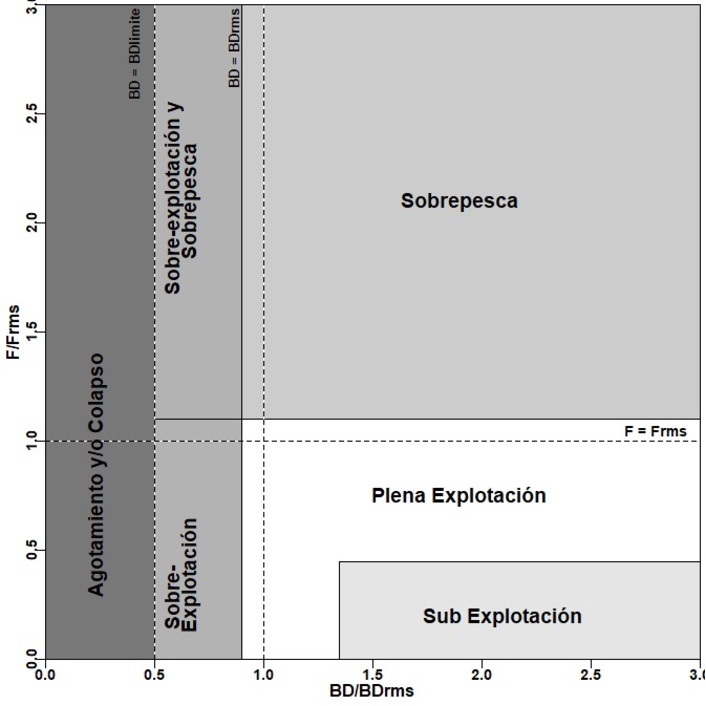
\includegraphics[width=0.8\textwidth]{Figuras/Fig8_InformeFinal.pdf}
\caption{Diagrama de fase definido por el CCT-PP para las pesquerías de pelágicos pequeños.}
\label{Fig8}
\end{figure}

\hypertarget{objetivo-especuxedfico-3}{%
\subsection{3.3. Objetivo específico
3:}\label{objetivo-especuxedfico-3}}

\vspace{-0.2cm}

\emph{``Determinar niveles de Captura Biológicamente Aceptable (CBA) que
lleven y/o mantenga la pesquería en torno al Rendimiento Máximo
Sostenible (RMS), a partir de un análisis de riesgo en condiciones de
incertidumbre de no alcanzar los objetivos de conservación y
sostenibilidad conforme lo establece la LGPA y contenidos en el Plan de
Manejo y/o en el Programa de Recuperación respectivo, según
corresponda.''} \vspace{0.5cm}

En base al modelo conceptual de la dinámica del stock respectivo que
sustenta el enfoque y modelo de evaluación aplicado, se realiza un
análisis de la productividad del stock y de sus posibilidades futuras de
explotación considerando los parámetros e indicadores estimados
precedentemente, con su incertidumbre asociada. El análisis considera
como criterio de explotación, aquel nivel de mortalidad que conduce al
Rendimiento Máximo Sostenido (\(F_{RMS}\)).

Se provee toda la información y antecedentes recopilados a objeto que
los correspondientes Comités Científico Técnicos (CCT) analicen los
resultados, considerando los requerimientos de reglas de decisión
establecidas en los Planes de Manejo o programas de recuperación
respectivos, conforme al marco legal y normativo vigente. Los análisis
consideran entre otros, la proyección poblacional bajo condiciones de
incertidumbre y la generación de tablas de decisión sobre las
consecuencias de determinadas acciones, junto al riesgo de no lograr
determinados objetivos.

\hypertarget{captura-bioluxf3gicamente-aceptable-cba-y-proyecciuxf3n-del-stock}{%
\subsubsection{3.3.1. Captura Biológicamente Aceptable (CBA) y
proyección del
stock}\label{captura-bioluxf3gicamente-aceptable-cba-y-proyecciuxf3n-del-stock}}

Las estimaciones de CBA y proyecciones de la biomasa se realizarán
utilizando el método de Zhou \emph{et al}. (2013) y se llevan a cabo
bajo un vector de valores (0,67; 1,0 y 1,25) multiplicadores del
\(F_{RMS}\), cuyo segundo valor del vector corresponde al \(F_{RMS}\).
La incertidumbre proviene del error asociado a la estimación de la
biomasa, los parámetros \(r\) y \(K\) se asumen constantes y
corresponden a aquellos valores que generan biomasas positivas y
consistentes con las capturas observadas. Se realiza una proyección del
stock al año 2021 para estimar la CBA del próximo año.

\hypertarget{objetivo-especuxedfico-4}{%
\subsection{3.4. Objetivo específico
4:}\label{objetivo-especuxedfico-4}}

\vspace{-0.2cm}

\emph{``Informar el avance del Programa de Mejoramiento Continuo de la
Calidad en la Asesoría Científica (PMCCAC) realizado durante el presente
estudio, respecto al cumplimiento de recomendaciones formuladas en
procesos de RPEI y priorizadas por el CCT, cuando corresponda.''}
\vspace{0.5cm}

Para el cumplimiento de este objetivo, se informan los avances
alcanzados durante el desarrollo del estudio, conforme al Programa de
Mejoramiento Continuo de la Calidad de la Asesoría Científica (PMCCAC),
elaborado para esta pesquería. Este PMCCAC se enfoca a las brechas de
datos, información y conocimiento, en relación con la situación general
de la pesquería acorde con los requerimientos de asesoría solicitados
por la administración pesquera.

\hypertarget{modelos-alternativos-para-determinaciuxf3n-de-estatus}{%
\subsubsection{3.4.1. Modelos alternativos para determinación de
Estatus}\label{modelos-alternativos-para-determinaciuxf3n-de-estatus}}

\hypertarget{a-spict-stochastic-surplus-production-model-in-continuous-time-peteresen-berg-2017}{%
\paragraph{a) SPiCT, Stochastic Surplus Production Model in Continuous
Time (Peteresen \& Berg,
2017)}\label{a-spict-stochastic-surplus-production-model-in-continuous-time-peteresen-berg-2017}}

\quad

SpiCT está formulado como un modelo de estado-espacio e incorpora
dinámicas relacionadas tanto con las pesquerías (\(F\)) como con la
biomasa (\(B\)) en la forma de Pella \& Tomlinson (1969). Estos dos
procesos latentes se relacionan luego con los datos observados (capturas
y captura por unidad de esfuerzo: CPUE, ya sea comercial o de
prospecciones) mediante ecuaciones de observación, que incluyen términos
de error. Se definen las ecuaciones del modelo;

Ecuaciones de proceso (random effects):

\begin{equation}
Biomasa: dB_t=rB_t\left(1-\left[\frac{B_t}{K}\right]^{n-1}\right)dt - F_t B_t dt + \sigma BB_tdW_t
\end{equation}

\begin{equation}
Pesca: d log(F_t)=f(t,\sigma F)
\end{equation}

En donde \(W_t\) es movimiento browniano (término de ruido)

Ecuaciones de observación:

\begin{equation}
Indice: logI_t=log(qB_t)+e_t, e_t\sim N\left(0,\left[\alpha \sigma B\right]^2\right)
\end{equation}

\begin{equation}
Captura: logC_t=log\left(\int_{t}^{t+\Delta}F_sB_sds\right)+e_t,
\end{equation}

\begin{equation}
e_t=N\left(0,\left[\beta \sigma F\right]^2\right)
\end{equation}

El modelo representado para la Mortalidad por Pesca mediante
\(F(t,\sigma F)\) cuando se usa el dato anual, como un \emph{random
walk} (o difusivo). Si existen series de datos sub-anuales, el modelo de
\(F\) incorpora un patrón estacional que es aplicado. La
\textbf{Tabla \ref{Tab5}} muestra los parámetros utilizado y sus
definiciones. \vspace{0.5cm}

\begin{longtable}[]{@{}ll@{}}
\caption{\label{Tab5} Parámetros y su descripción utilizados en el
modelo SPiCt para sardina austral de la Región de Aysén.}\tabularnewline
\toprule
\begin{minipage}[b]{0.14\columnwidth}\raggedright
Parámetro\strut
\end{minipage} & \begin{minipage}[b]{0.80\columnwidth}\raggedright
Definición\strut
\end{minipage}\tabularnewline
\midrule
\endfirsthead
\toprule
\begin{minipage}[b]{0.14\columnwidth}\raggedright
Parámetro\strut
\end{minipage} & \begin{minipage}[b]{0.80\columnwidth}\raggedright
Definición\strut
\end{minipage}\tabularnewline
\midrule
\endhead
\begin{minipage}[t]{0.14\columnwidth}\raggedright
\(B_t\)\strut
\end{minipage} & \begin{minipage}[t]{0.80\columnwidth}\raggedright
Biomasa del stock explotable\strut
\end{minipage}\tabularnewline
\begin{minipage}[t]{0.14\columnwidth}\raggedright
\(F_t\)\strut
\end{minipage} & \begin{minipage}[t]{0.80\columnwidth}\raggedright
Mortalidad por pesca\strut
\end{minipage}\tabularnewline
\begin{minipage}[t]{0.14\columnwidth}\raggedright
\(r\)\strut
\end{minipage} & \begin{minipage}[t]{0.80\columnwidth}\raggedright
Tasa intrínseca de crecimiento poblacional\strut
\end{minipage}\tabularnewline
\begin{minipage}[t]{0.14\columnwidth}\raggedright
\(K\)\strut
\end{minipage} & \begin{minipage}[t]{0.80\columnwidth}\raggedright
Capacidad de carga o biomasa de equilibrio en condición virginal\strut
\end{minipage}\tabularnewline
\begin{minipage}[t]{0.14\columnwidth}\raggedright
\(n\)\strut
\end{minipage} & \begin{minipage}[t]{0.80\columnwidth}\raggedright
Parámetro que determina la forma de la curva de producción\strut
\end{minipage}\tabularnewline
\begin{minipage}[t]{0.14\columnwidth}\raggedright
\(q\)\strut
\end{minipage} & \begin{minipage}[t]{0.80\columnwidth}\raggedright
Capturabilidad\strut
\end{minipage}\tabularnewline
\begin{minipage}[t]{0.14\columnwidth}\raggedright
\(\sigma_B\)\strut
\end{minipage} & \begin{minipage}[t]{0.80\columnwidth}\raggedright
Desviación estándar de \(B_t\)\strut
\end{minipage}\tabularnewline
\begin{minipage}[t]{0.14\columnwidth}\raggedright
\(\sigma_F\)\strut
\end{minipage} & \begin{minipage}[t]{0.80\columnwidth}\raggedright
Desviación estándar de \(F_t\)\strut
\end{minipage}\tabularnewline
\begin{minipage}[t]{0.14\columnwidth}\raggedright
\(\alpha\)\strut
\end{minipage} & \begin{minipage}[t]{0.80\columnwidth}\raggedright
Razón de desviación estándar de \(I_t\) para desviación estándar de
\(B_t\)\strut
\end{minipage}\tabularnewline
\begin{minipage}[t]{0.14\columnwidth}\raggedright
\(\beta\)\strut
\end{minipage} & \begin{minipage}[t]{0.80\columnwidth}\raggedright
Razón de desviación estándar de \(C_t\) para desviación estándar de
\(F_t\)\strut
\end{minipage}\tabularnewline
\bottomrule
\end{longtable}

Con información limitada, a menudo es difícil estimar \(n\), en cuyo
caso \(n\) se establece en 2 dando como resultado el modelo de Schaefer.
De manera similar, no siempre es posible estimar \(\alpha\) y/o
\(\beta\), en cuyo caso se establecen en 1, que es un supuesto común
(Thorson \emph{et al}., 2013). Sin embargo, este valor predeterminado
asume el mismo error en la captura y del índice, lo que se desvía de los
modelos de error de observación más simples que asumen que no hay error
en la captura pero que pueden ser apropiados para poblaciones con datos
limitados. SpiCT puede realizar proyecciones a corto plazo de la
biomasa, así como de la mortalidad por pesca y las capturas, incluida la
incertidumbre.

La configuración predeterminada de SpiCT estima todos los parámetros,
pero las configuraciones más simples fijan los parámetros \(n\) = 2,
\(\alpha\), \(\beta\) = 1, así como \(B_0/K\) (la relación entre la
biomasa inicial y la capacidad de carga).

Los supuestos de modelos importantes compartidos por todos los modelos
de producción incluyen:

\begin{itemize}
\item
  No se produce ninguna migración dentro y fuera de la población, ya que
  los cambios en la biomasa solo se producen a través del crecimiento a
  través de \(r\) y \(K\) y mediante la pesca.
\item
  Sin efectos rezagados en la dinámica de la biomasa causados por la
  variabilidad de la distribución por tamaño, edad y sexo.
\item
  Capacidad de captura constante, es decir ningún cambio en la
  tecnología de la técnica de pesca que cambia \(q\).
\item
  La selectividad puede seguir cualquier patrón siempre que sea
  constante en el tiempo.
\item
  No se requiere ningún conocimiento de la mortalidad natural porque
  está incluida en la tasa de crecimiento intrínseca, \(r\).
\item
  No existe un subregistro sistemático de captura y esfuerzo. Un modelo
  de producción puede o no ser robusto ante el fracaso de este supuesto.
  Por ejemplo, si la captura y el esfuerzo se subestiman en la misma
  cantidad durante toda la serie de tiempo, las estimaciones de
  \(B/B_{RMS}\), \(F/F_{RMS}\) y \(captura/RMS\) son válidas incluso si
  la captura, el \(RMS\) y la biomasa están subestimadas.
\end{itemize}

Además de las estimaciones de los parámetros, el modelo proporciona
estimaciones de los puntos biológicos de referencia \(B_{RMS}\),
\(F_{RMS}\) y \(RMS\), donde \(B_{RMS}\) es la biomasa que conduce a la
producción de excedente máxima (es decir, \(RMS\)), de manera similar
\(F_{RMS}\) es la mortalidad por pesca que conduce a \(RMS\). Todas las
estimaciones de los puntos de referencia incluyen incertidumbre
(intervalos de confianza del 95\%). Un beneficio adicional del paquete
TMB es que los residuales de un paso adelante se proporcionan
automáticamente, que deben ser independientes y distribuidos normalmente
de manera estándar para que la salida del modelo sea válida. Las
desviaciones de la independencia y la normalidad estándar de los
residuos indican que se han violado los supuestos del modelo. Por lo
tanto, es importante informar los diagnósticos residuales junto con los
resultados del modelo de manera que se puedan realizar interpretaciones
correctas. El SPiCT se implementa como un paquete R (R-Core Team, 2015)
y usa el paquete Template Model Builder (TMB, Kristensen \emph{et al}.
2015) para obtener una estimación de modelo rápida y eficiente.
\url{https://github.com/mawp/spict}.

\hypertarget{b-lbpa-length-based-pseudocohort-analysis-canales-et-al.-2020}{%
\paragraph{\texorpdfstring{b) LBPA, Length-Based Pseudocohort Analysis
(Canales \emph{et al}.,
2020)}{b) LBPA, Length-Based Pseudocohort Analysis (Canales et al., 2020)}}\label{b-lbpa-length-based-pseudocohort-analysis-canales-et-al.-2020}}

\quad

El método de evaluación de poblaciones marinas con datos limitados
llamado ``Análisis de pseudocohortes basado en la talla'' (Length-Based
Pseudocohort Analysis, LBPA por sus siglas en inglés) (Canales \emph{et
al}., 2021) ajusta cohortes por recluta para capturar datos de
frecuencia de talla, principalmente para estimar la selectividad en
función de la edad, la tasa de mortalidad por pesca (F) completamente
seleccionada y la proporción actual de biomasa virgen reproductora por
recluta (SPR) (Brooks \emph{et al}., 2010; Hordyk \emph{et al}., 2016).
El modelo supone que la población está en equilibrio y se puede ajustar
a varios años de datos de estructuras de tallas simultáneamente.

LBPA se basa en la supervivencia por recluta en función de la edad
(\(N_a\)), dada la mortalidad natural (\(M\)) y la mortalidad por pesca
específica por edad, es decir:

\begin{equation}
N_a = \left\lbrace
\begin{array}{ll}
1 & \textup{si } a=a_r\\
N_{a-1}S_{a-1} & \textup{si} a_r < A < A_+ \\
N_a(1-S_a) & \textup{si} a = A_+
\end{array}
\right.
\end{equation}

\begin{equation}
S_a= e^{-F_a-M}
\end{equation}

donde \(a\) es la edad, \(A_+\) es el grupo plus, \(F_a\) es la
mortalidad por pesca por edad (basada en el supuesto de separabilidad),
y \(\varphi_a\) es la selectividad por edad. La selectividad específica
por edad se deriva de la selectividad específica por talla
\(\varphi_i\), que es una función logística de la talla:

\begin{equation}
F_a=\varphi_a*F
\end{equation}

\begin{equation}
\varphi_a=\sum_{l}\pi_{a,l}\left(1+e^{-log(19) \left[\frac{l-L_{50}}{\Delta}\right]}\right)^{-1}
\end{equation}

donde \(L_a\) es la talla esperada para el grupo de edad \(a\), \(L_50\)
es la talla a la que el 50\% de los individuos son reclutados en la
pesquería y \(\delta\) es un parámetro de pendiente (la diferencia entre
tallas al 50\% y 95\% de selectividad).

\begin{equation}
\pi_{a,l}=\int_{l_i}^{l_{i+1}}e^{-0,5\left(\frac{l-l_a}{\delta_a}\right)^2}dl
\end{equation}

donde \(\pi_{a,l}\), \(l\) se determina usando la ecuación de
crecimiento de von Bertanlanfy parametrizada en términos de \(L_\infty\)
y \(k\), y el coeficiente de variación de la talla a la edad (\(cv\))
asumido es igual a 0.1. Este último supuesto se basa en (Prince \emph{et
al}. (2015) y Hordyk \emph{et al}. (2015), sin embargo, podría estimarse
junto con los demás parámetros del modelo.

\begin{equation}
L_a=L_{a-1}e^{-k}+L_\infty\left(1-e^{-k}\right)
\end{equation}

\begin{equation}
\delta_a = cv L_a
\end{equation}

donde el tamaño promedio inicial define el tamaño a la edad de
reclutamiento \(L_a = L_{a,r}\), Los parámetros pre-especificados y
estimados. La ecuación de captura de Baranov se usa para calcular la
composición por edad de captura, que luego se convierte a tallas (\(l\))
usando una matriz de probabilidad de talla por edad \(\pi_a\).

\begin{equation}
C_a=\left(\frac{F_a}{F_a+M}\right)N_a\left(1-S_a\right)
\end{equation}

\begin{equation}
\hat{C}_l=\sum_{a}C_a\pi_{a,l}
\end{equation}

La biomasa reproductora por recluta (\(SBPR\)) se calcula como:

\begin{equation}
SSBPR=\sum_{l}\left(\sum_{a}\left(N_a e^{-\gamma Z_a}\right)\pi_{a,l}\right)O_lw_l
\end{equation}

Donde la mortalidad total es \(Z_a=F_a+M\) es la mortalidad
total,\(\gamma\) =0,875 es la fracción del año de desove, \(O_i\) es la
proporción de animales de longitud \(l\) que están maduros y \(w_t\) es
el peso promedio en longitud. La biomasa virgen de desove por recluta
\(SSBPR_0\) se calcula cuando (\(Z = M\)). La relación de potencial de
desove (\(SPR\)) es \(SSBPR/SSBPR_0\).

Los parámetros (\(\theta = \left[F,A_{50},\Delta,L_{a_r}\right]\)) se
estimaron utilizando la máxima verosimilitud penalizada (De Valpine y
Hilborn, 2005; Methot y Taylor, 2011; Hutchinson \emph{et al}., 2015).
Se asumió que los datos de frecuencia de tallas eran multinomiales,
mientras que los parámetros estimados (\(\theta\)) se penalizaron (en
espacio logarítmico) utilizando un marco semi-Bayesiano (Cole \emph{et
al}., 2013).

\begin{equation}
ll=-\dot{N}\sum_{y}\lambda_y\sum_{l}p_{l,y}log(\hat{p}_l)+\sum_{j}\left(\frac{log(\theta_j)-log(\hat{\theta}_j)}{\sigma_{\theta_j}}\right)^2
\end{equation}

donde \(N\) es el tamaño efectivo de la muestra (por ejemplo,
\(\dot{N}\) = 100), \(p_{l,y}\) es la proporción de la captura en el año
\(y\) en la clase de talla \(l\), \(\hat{p}_{l,y}\) es la proporción de
la captura predicha por el modelo año y en la clase de talla \(l\) (se
supone que se aplica a todos los años), y \(\lambda_y\) es un factor de
ponderación para los datos de frecuencia de talla para el año \(y\). El
segundo término son las penalizaciones del modelo, donde \(\theta_j\) es
el valor a priori del \emph{j-ésimo} parámetro del modelo y
\(\sigma_{\theta_j}\) es la desviación estándar de la \emph{j-ésima}
penalización del parámetro en el espacio logarítmico. LBPA es
implementado en ADMB (www.admb-project.org) y todas sus salidas son
leídas en R.

\pagebreak
\normalsize

\hypertarget{resultados}{%
\section{4. RESULTADOS}\label{resultados}}

\hypertarget{objetivo-especuxedfico-1-1}{%
\subsection{4.1. Objetivo específico
1:}\label{objetivo-especuxedfico-1-1}}

\vspace{-0.2cm}

\emph{``Implementarprocedimientosdeevaluacióndestockbasadosenprotocoloscientíficosparala
determinación del estatus de los recursos seleccionados con arreglo al
nivel de conocimiento, información e incertidumbre correspondiente,
conforme a los estándares actuales en ciencia pesquera.''}
\vspace{0.5cm}

\hypertarget{datos-de-entrada-al-modelo-de-evaluaciuxf3n-de-stock-1}{%
\subsubsection{4.1.1. Datos de entrada al modelo de evaluación de
stock}\label{datos-de-entrada-al-modelo-de-evaluaciuxf3n-de-stock-1}}

\hypertarget{desembarques-y-crucero-de-evaluaciuxf3n-acuxfastica}{%
\paragraph{Desembarques y crucero de evaluación
acústica}\label{desembarques-y-crucero-de-evaluaciuxf3n-acuxfastica}}

\quad

En la región de Aysén, la pesquería de sardina austral muestra una
actividad esporádica y de menor intensidad en comparación a la región de
Los Lagos. Solo entre 2 a 10 naves han declarado desembarque de la
especien en la zona. Se cuenta con registros oficiales de desembarque a
partir del año 2012 (SERNAPESCA, www.sernapesca.cl). Estos, han oscilado
en valores promedio de 5 mil t, entre el año 2012 y 2017. El año 2015 se
registró el valor más alto con 7,5 mil t. El año 2018 en cambio, la
actividad fue escasa y alcanzó un mínimo valor de 653. El año 2019 se
aprecia un incremento hasta las 1352 t y la expectativa de captura para
el 2020 (supuesto de desembarque) alcanza valores cercanos a las 2900 t.
La biomasa del crucero muestra una reducción importante desde 100 mil t
el año 2013 hasta 6,5 mil t el año 2019 ( \textbf{Figura \ref{Fig9}}).
El año 2020, no se realizó el crucero en esta zona. \vspace{0.5cm}

\begin{figure}[h!]
\centering
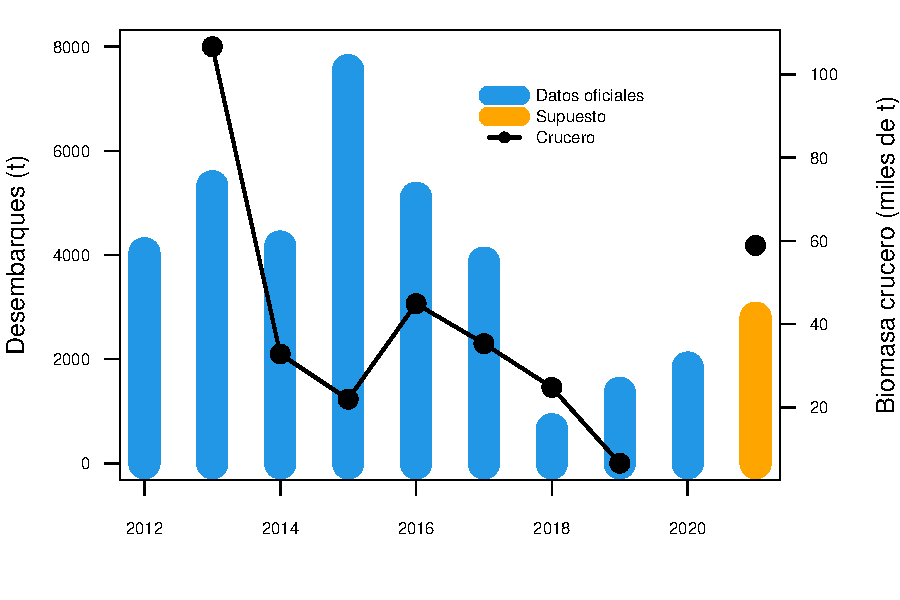
\includegraphics[width=0.8\textwidth]{Figuras/Fig9_InformeFinal-1.pdf}
\caption{Desembarques de sardina austral en la Región de Aysén (fuente: Sernapesca) y biomasa estimada en el crucero de evaluación directa.}
\label{Fig9}
\end{figure}

\hypertarget{muxe9todo-de-hilborn-mangel-1997-1}{%
\paragraph{4.1.2. Método de Hilborn \& Mangel
1997}\label{muxe9todo-de-hilborn-mangel-1997-1}}

\quad

El período de análisis de la evaluación de stock actual, abarca los años
2012 a 2020, con información completa de las piezas de información hasta
el año 2020. Los índices que se utilizan en dicho modelo, corresponden a
la información de desembarques oficiales (Sernapesca) y biomasa del
crucero (\(B_{cru}\)) de evaluación directa desarrollado por IFOP en
aguas interiores de la Región de Aysén.

El resultado más relevante del presente análisis se relaciona con el
nivel de depleción (D) estimado para el stock (
\textbf{Figura \ref{Fig10}}), ya que ha sido utilizado en la metodología
de Zhou \emph{et al}., (2013) que es presentado actualmente al Comité
Científico de pequeños pelágicos para definir el estatus del recurso en
la Región de Aysén. En términos de reducción, al usar toda la
información disponible, los resultados indican que, durante el 2020, el
stock estaría reducido hasta un 26\% de su condición original el año
2013 (\textbf{Tabla \ref{Tab6}}). A pesar de estos resultados, la
actividad de la flota durante los últimos meses del 2019 y los primeros
del 2020, muestran una recuperación importante en sus capturas. Hasta
mayo del año en curso, se había desembarcado el 97\% de la cuota
asignada inicialmente para esta zona. Esto hace suponer una condición
menos pesimista del stock que el nivel de depleción (0,26) estimado en
el presente análisis. Asimismo, a pesar que el año 2020 no se realizó el
estudio de evaluación directa en la Región de Aysén, el incremento en la
biomasa detectado por el crucero en la Región de Los Lagos, hace suponer
un incremento también en el stock del sur (Aysén). Este supuesto se basa
en la similitud histórica en la variabilidad del índice acústico en
ambas zonas de evaluación. De esta manera, considerando los antecedentes
previos, se utiliza en la metodología de Zhou \emph{et al}. (2013) un
nivel máximo de agotamiento (D) o reducción del stock de la población de
0,5.

\vspace{0.5cm}

\begin{figure}[h!]
\centering
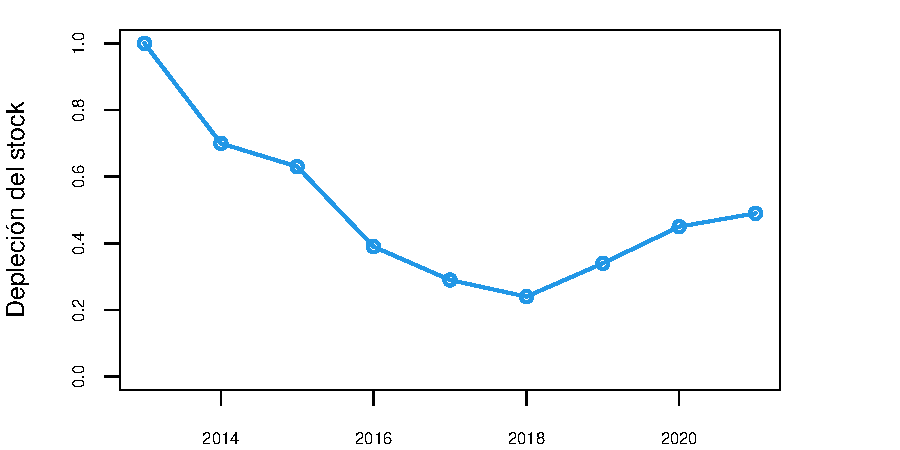
\includegraphics[width=0.8\textwidth]{Figuras/Fig10_InformeFinal-1.pdf}
\caption{Índice de depleción del stock según la metodología de Hilbor y Mangel (1997) para sardina austral en aguas interiores de la Región de Aysén.}
\label{Fig10}
\end{figure}

\vspace{0.5cm}

\begin{longtable}[]{@{}ccc@{}}
\caption{\label{Tab6} Biomasa (B) y reducción del stock (D) según la
metodología de Hilbor y Mangel (1997) para sardina austral en aguas
interiores de la Región de Aysén.}\tabularnewline
\toprule
\begin{minipage}[b]{0.09\columnwidth}\centering
Año\strut
\end{minipage} & \begin{minipage}[b]{0.13\columnwidth}\centering
Biomasa\strut
\end{minipage} & \begin{minipage}[b]{0.16\columnwidth}\centering
Depleción\strut
\end{minipage}\tabularnewline
\midrule
\endfirsthead
\toprule
\begin{minipage}[b]{0.09\columnwidth}\centering
Año\strut
\end{minipage} & \begin{minipage}[b]{0.13\columnwidth}\centering
Biomasa\strut
\end{minipage} & \begin{minipage}[b]{0.16\columnwidth}\centering
Depleción\strut
\end{minipage}\tabularnewline
\midrule
\endhead
\begin{minipage}[t]{0.09\columnwidth}\centering
2013\strut
\end{minipage} & \begin{minipage}[t]{0.13\columnwidth}\centering
17.712\strut
\end{minipage} & \begin{minipage}[t]{0.16\columnwidth}\centering
1,00\strut
\end{minipage}\tabularnewline
\begin{minipage}[t]{0.09\columnwidth}\centering
2014\strut
\end{minipage} & \begin{minipage}[t]{0.13\columnwidth}\centering
12.394\strut
\end{minipage} & \begin{minipage}[t]{0.16\columnwidth}\centering
0,70\strut
\end{minipage}\tabularnewline
\begin{minipage}[t]{0.09\columnwidth}\centering
2015\strut
\end{minipage} & \begin{minipage}[t]{0.13\columnwidth}\centering
11.186\strut
\end{minipage} & \begin{minipage}[t]{0.16\columnwidth}\centering
0,63\strut
\end{minipage}\tabularnewline
\begin{minipage}[t]{0.09\columnwidth}\centering
2016\strut
\end{minipage} & \begin{minipage}[t]{0.13\columnwidth}\centering
6.911\strut
\end{minipage} & \begin{minipage}[t]{0.16\columnwidth}\centering
0,39\strut
\end{minipage}\tabularnewline
\begin{minipage}[t]{0.09\columnwidth}\centering
2017\strut
\end{minipage} & \begin{minipage}[t]{0.13\columnwidth}\centering
5.161\strut
\end{minipage} & \begin{minipage}[t]{0.16\columnwidth}\centering
0,29\strut
\end{minipage}\tabularnewline
\begin{minipage}[t]{0.09\columnwidth}\centering
2018\strut
\end{minipage} & \begin{minipage}[t]{0.13\columnwidth}\centering
4.212\strut
\end{minipage} & \begin{minipage}[t]{0.16\columnwidth}\centering
0,24\strut
\end{minipage}\tabularnewline
\begin{minipage}[t]{0.09\columnwidth}\centering
2019\strut
\end{minipage} & \begin{minipage}[t]{0.13\columnwidth}\centering
6.108\strut
\end{minipage} & \begin{minipage}[t]{0.16\columnwidth}\centering
0,34\strut
\end{minipage}\tabularnewline
\begin{minipage}[t]{0.09\columnwidth}\centering
2020\strut
\end{minipage} & \begin{minipage}[t]{0.13\columnwidth}\centering
7.933\strut
\end{minipage} & \begin{minipage}[t]{0.16\columnwidth}\centering
0,45\strut
\end{minipage}\tabularnewline
\begin{minipage}[t]{0.09\columnwidth}\centering
2021\strut
\end{minipage} & \begin{minipage}[t]{0.13\columnwidth}\centering
8.592\strut
\end{minipage} & \begin{minipage}[t]{0.16\columnwidth}\centering
0,49\strut
\end{minipage}\tabularnewline
\bottomrule
\end{longtable}

\normalsize 
\pagebreak

\hypertarget{objetivo-especuxedfico-2-1}{%
\subsection{4.2. Objetivo específico
2:}\label{objetivo-especuxedfico-2-1}}

\vspace{-0.2cm}

\emph{``Establecer el estatus actualizado de estos recursos, sobre la
base de sus principales indicadores estandarizados de estado y flujo,
incorporando, cuantificando y propagando la incertidumbre subyacente a
la pesquería.''} \vspace{0.5cm}

\hypertarget{indicadores-del-stock-muxe9todo-de-zhou}{%
\subsubsection{4.2.1. Indicadores del stock (Método de
Zhou)}\label{indicadores-del-stock-muxe9todo-de-zhou}}

Para la actualización de la evaluación de stock de sardina austral en
aguas interiores de la Región de Aysén, respecto del primer hito de
evaluación, se actualizó la información de desembarques hasta el año
2020 (valor supuesto) (\textbf{Tabla \ref{Tab7}}). Se consideró además
para este análisis un nivel máximo de agotamiento (D) o reducción del
stock de la población de 0,5. Este nivel asumido, se basa en la
recuperación de las capturas de la flota los últimos meses del año 2019
y los primeros del 2020 y difiere del valor estimado en el actual
estudio (0,26) a través de la metodología de Hilborn y Mangel (1997).

\vspace{0.5cm}

\begin{longtable}[]{@{}cc@{}}
\caption{\label{Tab7} Datos de captura usados en cada hito para la
evaluación de stock de sardina austral en aguas interiores de la Región
de Aysén a través de la metodología de Zhou (2013).}\tabularnewline
\toprule
\begin{minipage}[b]{0.14\columnwidth}\centering
Año\strut
\end{minipage} & \begin{minipage}[b]{0.18\columnwidth}\centering
Desembarque\strut
\end{minipage}\tabularnewline
\midrule
\endfirsthead
\toprule
\begin{minipage}[b]{0.14\columnwidth}\centering
Año\strut
\end{minipage} & \begin{minipage}[b]{0.18\columnwidth}\centering
Desembarque\strut
\end{minipage}\tabularnewline
\midrule
\endhead
\begin{minipage}[t]{0.14\columnwidth}\centering
2012\strut
\end{minipage} & \begin{minipage}[t]{0.18\columnwidth}\centering
4.033\strut
\end{minipage}\tabularnewline
\begin{minipage}[t]{0.14\columnwidth}\centering
2013\strut
\end{minipage} & \begin{minipage}[t]{0.18\columnwidth}\centering
5.318\strut
\end{minipage}\tabularnewline
\begin{minipage}[t]{0.14\columnwidth}\centering
2014\strut
\end{minipage} & \begin{minipage}[t]{0.18\columnwidth}\centering
4.163\strut
\end{minipage}\tabularnewline
\begin{minipage}[t]{0.14\columnwidth}\centering
2015\strut
\end{minipage} & \begin{minipage}[t]{0.18\columnwidth}\centering
7.547\strut
\end{minipage}\tabularnewline
\begin{minipage}[t]{0.14\columnwidth}\centering
2016\strut
\end{minipage} & \begin{minipage}[t]{0.18\columnwidth}\centering
5.097\strut
\end{minipage}\tabularnewline
\begin{minipage}[t]{0.14\columnwidth}\centering
2017\strut
\end{minipage} & \begin{minipage}[t]{0.18\columnwidth}\centering
3.853\strut
\end{minipage}\tabularnewline
\begin{minipage}[t]{0.14\columnwidth}\centering
2018\strut
\end{minipage} & \begin{minipage}[t]{0.18\columnwidth}\centering
653\strut
\end{minipage}\tabularnewline
\begin{minipage}[t]{0.14\columnwidth}\centering
2019\strut
\end{minipage} & \begin{minipage}[t]{0.18\columnwidth}\centering
1.352\strut
\end{minipage}\tabularnewline
\begin{minipage}[t]{0.14\columnwidth}\centering
2020\strut
\end{minipage} & \begin{minipage}[t]{0.18\columnwidth}\centering
1.839\strut
\end{minipage}\tabularnewline
\bottomrule
\end{longtable}

\vspace{0.5cm}

Se presentan las estimaciones de biomasa de sardina austral en la Región
de Aysén para el período 2012 al 2020 (\textbf{Figura \ref{Fig11}}). De
acuerdo a los resultados del modelo de evaluación actualizado, la
biomasa total (BT) evidenció una importante reducción desde 16,7 mil t
al inicio de la serie (2012) hasta 3,4 mil t el año 2018. Este último
año, la reducción poblacional, alcanzó un mínimo valor de 21\% respecto
al año 2012. Los años 2019 y 2020, el stock muestra una recuperación en
el nivel de biomasa, presentando un nivel de reducción del 45\% respecto
de su condición inicial. Desde el inicio de la serie, la tasa de
mortalidad por pesca se incrementa considerablemente desde 0,24
año\textsuperscript{-1} hasta de 0.88 año\textsuperscript{-1} el año
2017. Luego se reduce fuertemente hasta 0,19 año\textsuperscript{-1} el
2018 y 0,25 año\textsuperscript{-1} el 2019. Esto, debido a la
disminución en el desembarque los últimos años. Durante el año 2020, el
nivel de F alcanzaría un valor de 0,38 año\textsuperscript{-1}, aunque
el último año se basa en un supuesto del nivel de captura.

\pagebreak

\begin{longtable}[]{@{}ccccccc@{}}
\caption{\label{Tab8} Tabla comparativa entre la evaluación previa
(septiembre 2020) y el actual análisis (junio 2021). Estimaciones de
biomasa (t), mortalidad por pesca (F) y reducción del stock (BT/Bo) para
sardina austral en aguas interiores de la región de Aysén entre los años
2012 y 2020 según el método de Zhou \emph{et al}. (2013)}\tabularnewline
\toprule
\begin{minipage}[b]{0.05\columnwidth}\centering
Año\strut
\end{minipage} & \begin{minipage}[b]{0.12\columnwidth}\centering
\(BT_{sept20}\)\strut
\end{minipage} & \begin{minipage}[b]{0.11\columnwidth}\centering
\(BT_{jun21}\)\strut
\end{minipage} & \begin{minipage}[b]{0.16\columnwidth}\centering
\(BT/B_{0_{sept20}}\)\strut
\end{minipage} & \begin{minipage}[b]{0.15\columnwidth}\centering
\(BT/B_{0_{jun21}}\)\strut
\end{minipage} & \begin{minipage}[b]{0.11\columnwidth}\centering
\(F_{sept20}\)\strut
\end{minipage} & \begin{minipage}[b]{0.11\columnwidth}\centering
\(F_{jun21}\)\strut
\end{minipage}\tabularnewline
\midrule
\endfirsthead
\toprule
\begin{minipage}[b]{0.05\columnwidth}\centering
Año\strut
\end{minipage} & \begin{minipage}[b]{0.12\columnwidth}\centering
\(BT_{sept20}\)\strut
\end{minipage} & \begin{minipage}[b]{0.11\columnwidth}\centering
\(BT_{jun21}\)\strut
\end{minipage} & \begin{minipage}[b]{0.16\columnwidth}\centering
\(BT/B_{0_{sept20}}\)\strut
\end{minipage} & \begin{minipage}[b]{0.15\columnwidth}\centering
\(BT/B_{0_{jun21}}\)\strut
\end{minipage} & \begin{minipage}[b]{0.11\columnwidth}\centering
\(F_{sept20}\)\strut
\end{minipage} & \begin{minipage}[b]{0.11\columnwidth}\centering
\(F_{jun21}\)\strut
\end{minipage}\tabularnewline
\midrule
\endhead
\begin{minipage}[t]{0.05\columnwidth}\centering
2012\strut
\end{minipage} & \begin{minipage}[t]{0.12\columnwidth}\centering
16.669\strut
\end{minipage} & \begin{minipage}[t]{0.11\columnwidth}\centering
16.735\strut
\end{minipage} & \begin{minipage}[t]{0.16\columnwidth}\centering
1,00\strut
\end{minipage} & \begin{minipage}[t]{0.15\columnwidth}\centering
1,01\strut
\end{minipage} & \begin{minipage}[t]{0.11\columnwidth}\centering
0,24\strut
\end{minipage} & \begin{minipage}[t]{0.11\columnwidth}\centering
0,24\strut
\end{minipage}\tabularnewline
\begin{minipage}[t]{0.05\columnwidth}\centering
2013\strut
\end{minipage} & \begin{minipage}[t]{0.12\columnwidth}\centering
12.608\strut
\end{minipage} & \begin{minipage}[t]{0.11\columnwidth}\centering
12.563\strut
\end{minipage} & \begin{minipage}[t]{0.16\columnwidth}\centering
0,76\strut
\end{minipage} & \begin{minipage}[t]{0.15\columnwidth}\centering
0,76\strut
\end{minipage} & \begin{minipage}[t]{0.11\columnwidth}\centering
0,42\strut
\end{minipage} & \begin{minipage}[t]{0.11\columnwidth}\centering
0,42\strut
\end{minipage}\tabularnewline
\begin{minipage}[t]{0.05\columnwidth}\centering
2014\strut
\end{minipage} & \begin{minipage}[t]{0.12\columnwidth}\centering
10.088\strut
\end{minipage} & \begin{minipage}[t]{0.11\columnwidth}\centering
10.136\strut
\end{minipage} & \begin{minipage}[t]{0.16\columnwidth}\centering
0,61\strut
\end{minipage} & \begin{minipage}[t]{0.15\columnwidth}\centering
0,61\strut
\end{minipage} & \begin{minipage}[t]{0.11\columnwidth}\centering
0,41\strut
\end{minipage} & \begin{minipage}[t]{0.11\columnwidth}\centering
0,41\strut
\end{minipage}\tabularnewline
\begin{minipage}[t]{0.05\columnwidth}\centering
2015\strut
\end{minipage} & \begin{minipage}[t]{0.12\columnwidth}\centering
9.655\strut
\end{minipage} & \begin{minipage}[t]{0.11\columnwidth}\centering
9.649\strut
\end{minipage} & \begin{minipage}[t]{0.16\columnwidth}\centering
0,58\strut
\end{minipage} & \begin{minipage}[t]{0.15\columnwidth}\centering
0,58\strut
\end{minipage} & \begin{minipage}[t]{0.11\columnwidth}\centering
0,78\strut
\end{minipage} & \begin{minipage}[t]{0.11\columnwidth}\centering
0,78\strut
\end{minipage}\tabularnewline
\begin{minipage}[t]{0.05\columnwidth}\centering
2016\strut
\end{minipage} & \begin{minipage}[t]{0.12\columnwidth}\centering
5.874\strut
\end{minipage} & \begin{minipage}[t]{0.11\columnwidth}\centering
5.931\strut
\end{minipage} & \begin{minipage}[t]{0.16\columnwidth}\centering
0,35\strut
\end{minipage} & \begin{minipage}[t]{0.15\columnwidth}\centering
0,36\strut
\end{minipage} & \begin{minipage}[t]{0.11\columnwidth}\centering
0,87\strut
\end{minipage} & \begin{minipage}[t]{0.11\columnwidth}\centering
0,86\strut
\end{minipage}\tabularnewline
\begin{minipage}[t]{0.05\columnwidth}\centering
2017\strut
\end{minipage} & \begin{minipage}[t]{0.12\columnwidth}\centering
4.371\strut
\end{minipage} & \begin{minipage}[t]{0.11\columnwidth}\centering
4.449\strut
\end{minipage} & \begin{minipage}[t]{0.16\columnwidth}\centering
0,26\strut
\end{minipage} & \begin{minipage}[t]{0.15\columnwidth}\centering
0,27\strut
\end{minipage} & \begin{minipage}[t]{0.11\columnwidth}\centering
0,88\strut
\end{minipage} & \begin{minipage}[t]{0.11\columnwidth}\centering
0,87\strut
\end{minipage}\tabularnewline
\begin{minipage}[t]{0.05\columnwidth}\centering
2018\strut
\end{minipage} & \begin{minipage}[t]{0.12\columnwidth}\centering
3.473\strut
\end{minipage} & \begin{minipage}[t]{0.11\columnwidth}\centering
3.598\strut
\end{minipage} & \begin{minipage}[t]{0.16\columnwidth}\centering
0,21\strut
\end{minipage} & \begin{minipage}[t]{0.15\columnwidth}\centering
0,22\strut
\end{minipage} & \begin{minipage}[t]{0.11\columnwidth}\centering
0,19\strut
\end{minipage} & \begin{minipage}[t]{0.11\columnwidth}\centering
0,18\strut
\end{minipage}\tabularnewline
\begin{minipage}[t]{0.05\columnwidth}\centering
2019\strut
\end{minipage} & \begin{minipage}[t]{0.12\columnwidth}\centering
5.372\strut
\end{minipage} & \begin{minipage}[t]{0.11\columnwidth}\centering
5.603\strut
\end{minipage} & \begin{minipage}[t]{0.16\columnwidth}\centering
0,32\strut
\end{minipage} & \begin{minipage}[t]{0.15\columnwidth}\centering
0,34\strut
\end{minipage} & \begin{minipage}[t]{0.11\columnwidth}\centering
0,25\strut
\end{minipage} & \begin{minipage}[t]{0.11\columnwidth}\centering
0,24\strut
\end{minipage}\tabularnewline
\begin{minipage}[t]{0.05\columnwidth}\centering
2020\strut
\end{minipage} & \begin{minipage}[t]{0.12\columnwidth}\centering
7.498\strut
\end{minipage} & \begin{minipage}[t]{0.11\columnwidth}\centering
7.798\strut
\end{minipage} & \begin{minipage}[t]{0.16\columnwidth}\centering
0,45\strut
\end{minipage} & \begin{minipage}[t]{0.15\columnwidth}\centering
0,47\strut
\end{minipage} & \begin{minipage}[t]{0.11\columnwidth}\centering
0,38\strut
\end{minipage} & \begin{minipage}[t]{0.11\columnwidth}\centering
0,24\strut
\end{minipage}\tabularnewline
\bottomrule
\end{longtable}

\vspace{0.5cm}

\begin{figure}[h!]
\centering
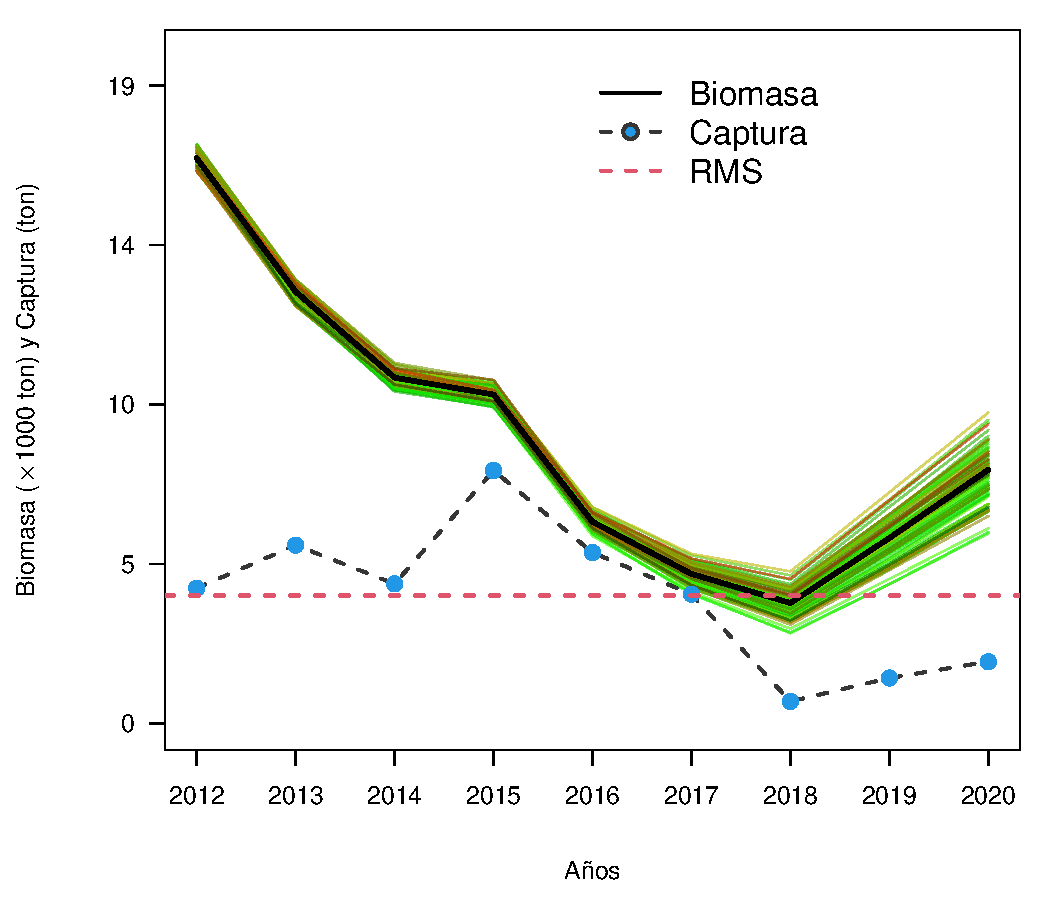
\includegraphics[width=0.7\textwidth]{Figuras/Fig1_Zhou2013_biomasa-1.pdf}
\caption{Estimaciones de biomasa total de sardina austral en la Región de Aysén a través de la aplicación del método de Zhou \textit{et al}. (2013) para el período entre 2012 y 2020. La línea negra representa el cuantil del 50\% de la distribución de biomasa proveniente de todas las combinaciones viables para $r$ y $K$. La línea segmentada roja representa el $RMS$ y los puntos azules las capturas observadas. Las líneas de colores muestran las posibles trayectorias de las posibles trayectorias de las biomasas.}
\label{Fig11}
\end{figure}

\pagebreak

El modelo de evaluación de Zhou \emph{et al}. (2013) fue sensibilizado
usando un vector de reducción (\(D\)) con valores entre 0,4 y 0,8. Los
resultados de este análisis de sensibilidad son presentados en la
\textbf{Figura \ref{Fig12}}. En general, a un nivel mayor de reducción
las estimaciones de biomasa total se hacen mayores con respecto a
aquellas estimaciones con un nivel inferior de reducción y los
intervalos de confianza se hacen más amplios. Para este análisis, se
consideró como escenario base el nivel de reducción de 0,4. Otra manera
de ver los resultados del análisis de sensibilidad es con respecto a los
parámetros estimados como una función de este nivel superior de
reducción asumido. La \textbf{Figura \ref{Fig13}} muestra los diferentes
parámetros (\(K\), \(r\), \(RMS\), \(D\)) en función del nivel superior
de reducción. Se aprecia que el parámetro \(r\), es estable y muestra
poca variación entre cada nivel de \(D\) asumida. \(K\) por su parte,
muestra mayor variación de niveles de \(D\) por sobre 0,6. Como es de
esperar, la condición del stock para el último año respecto del inicio
de la serie es altamente dependiente del nivel de reducción asumido.

\vspace{0.5cm}

\begin{figure}[h!]
\centering
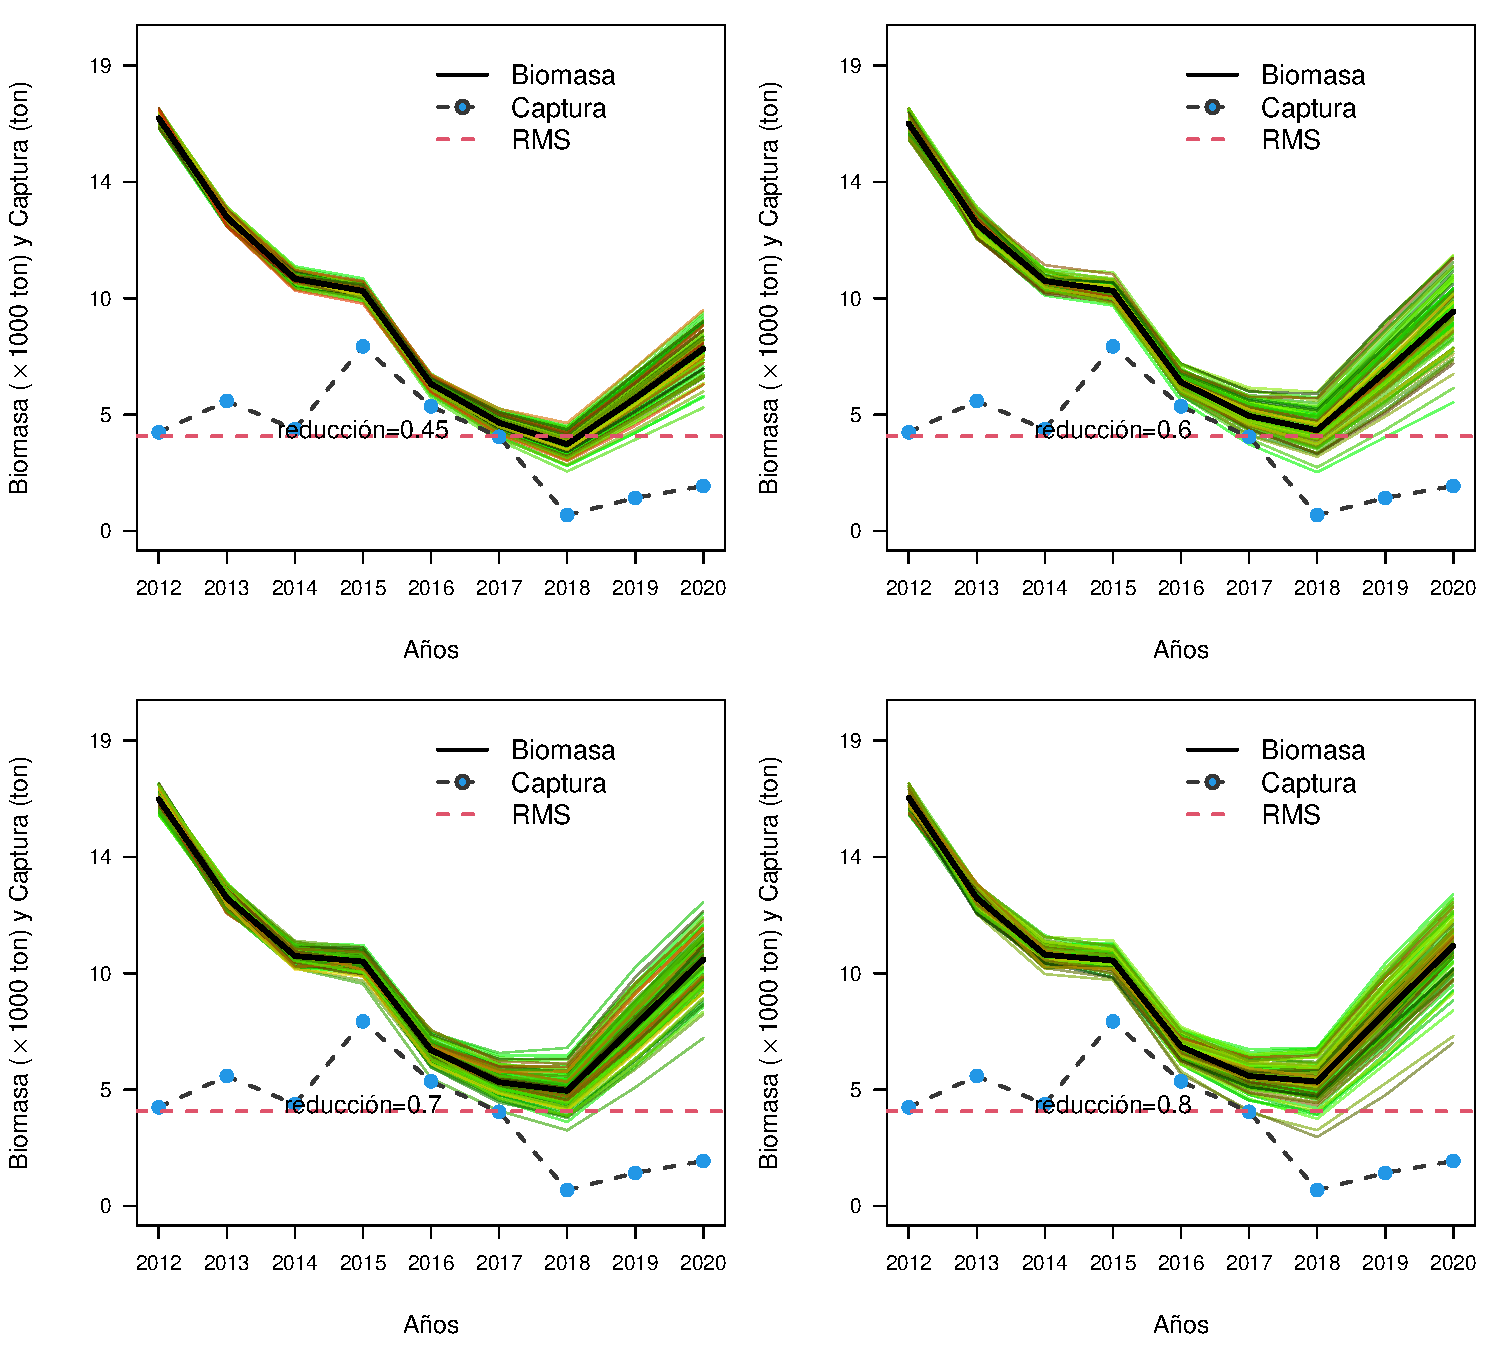
\includegraphics[width=0.95\textwidth]{Figuras/Fig2_Zhou2013_depletion-1.pdf}
\caption{Análisis de sensibilidad del método de Zhou \textit{et al}. (2013) para las estimaciones de biomasa total, asumiendo diferentes niveles máximos de reducción del stock. La línea negra representa el cuantil del 50\% de la distribución de biomasa. La línea horizontal segmentada roja representa el RMS y los puntos azules las capturas observadas. Las líneas de colores muestran las posibles trayectorias de las biomasas.}
\label{Fig12}
\end{figure}

\pagebreak

\begin{figure}[h!]
\centering
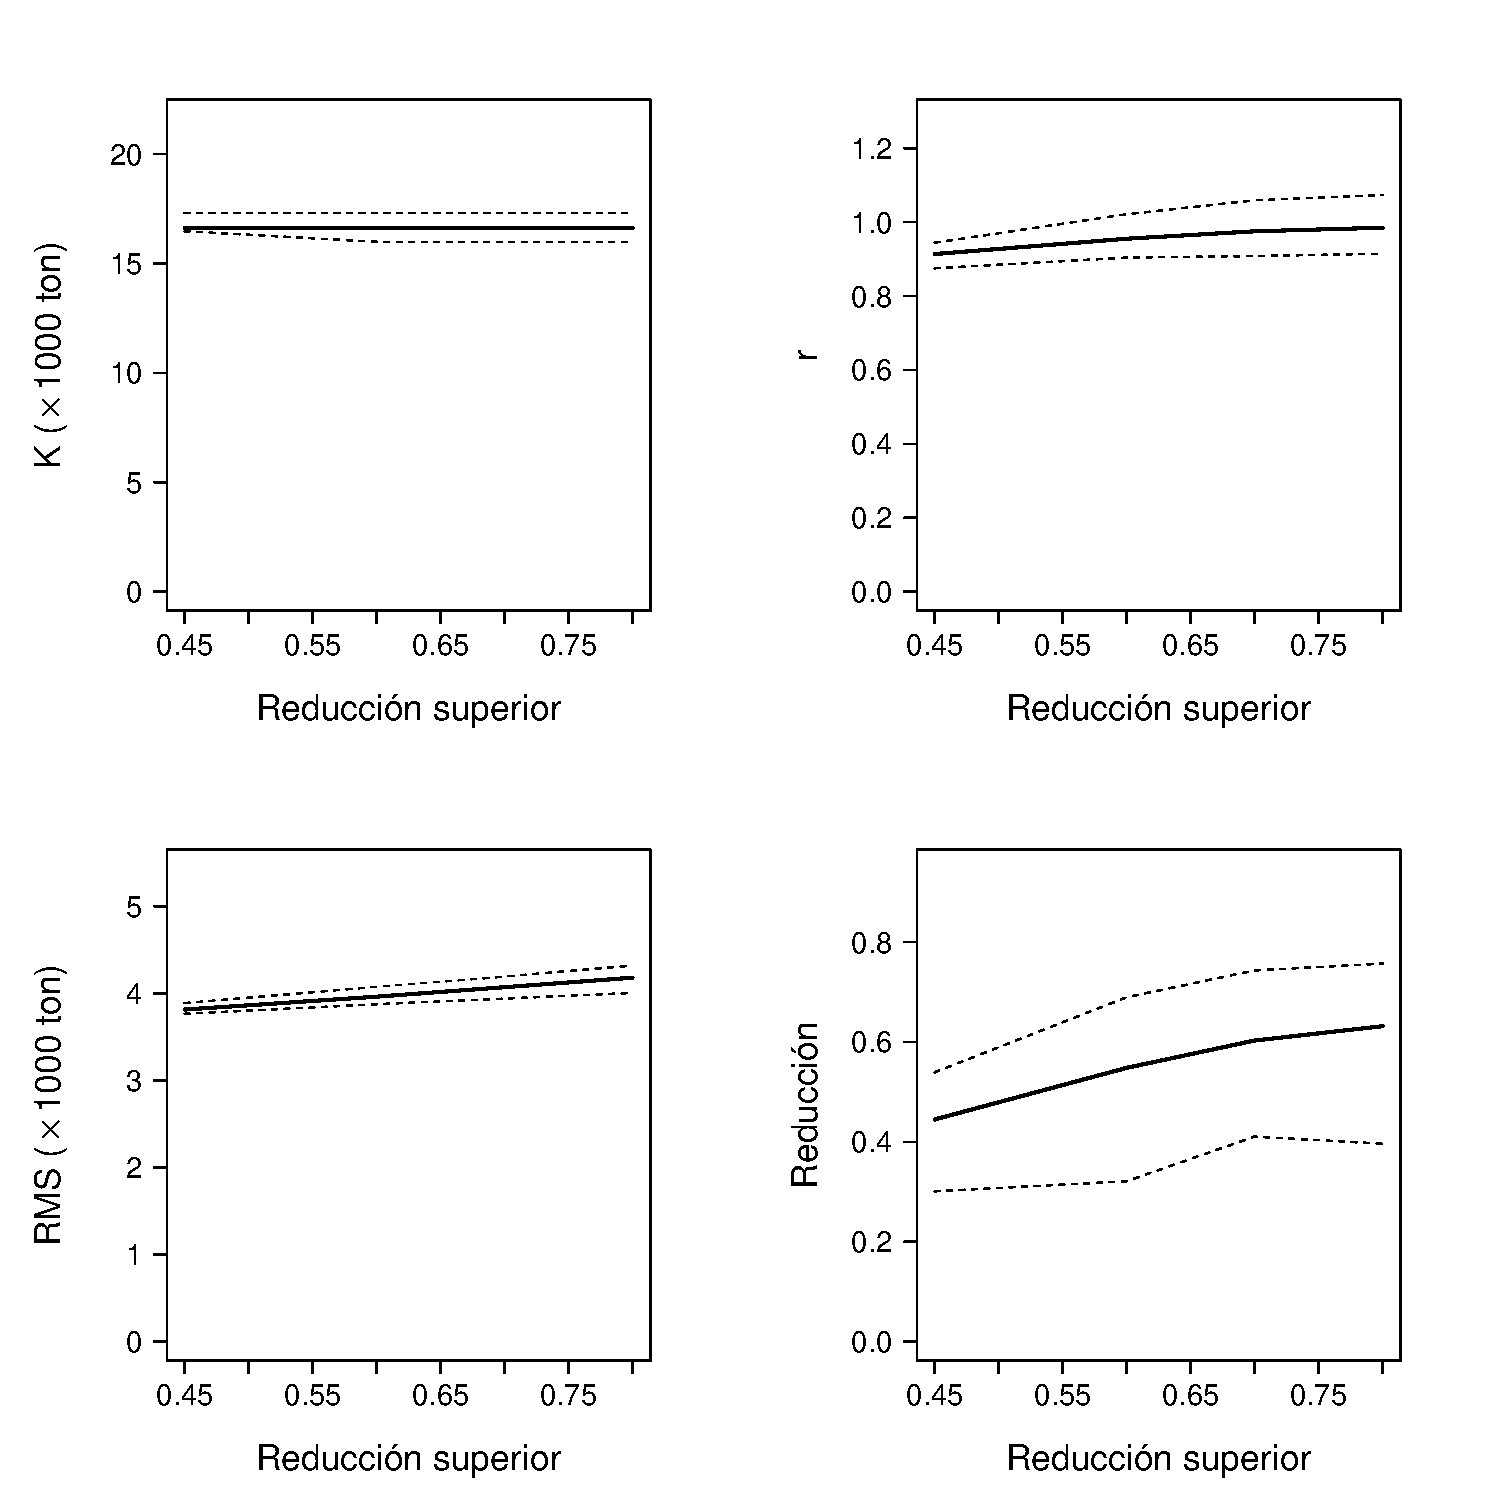
\includegraphics[width=1\textwidth]{Figuras/Fig3_Zhou2013_sensitivity-1.pdf}
\caption{Análisis de sensibilidad del método de Zhou \textit{et al}. (2013) para las estimaciones de los diferentes parámetros en función de un nivel superior de reducción asumido. La línea negra representa el cuantil del 50\% de la estimación para cada parámetro. Las líneas segmentadas representan el cuantil del 25\% y 75\% de las estimaciones.}
\label{Fig13}
\end{figure}

\pagebreak

\hypertarget{estado-de-explotaciuxf3n}{%
\subsubsection{4.2.2. Estado de
explotación}\label{estado-de-explotaciuxf3n}}

\quad

Los puntos biológicos de referencia basados en el modelo de evaluación
de Zhou \emph{et al}. (2013), indican que la biomasa al máximo
rendimiento sostenido corresponde, según el actual análisis a 8,32 mil
toneladas, la mortalidad por pesca (F) al máximo rendimiento sostenido
es de 0,46 año\textsuperscript{-1} y el rendimiento máximo sostenido
estimado por este método debería estar en torno a las 3.85 mil toneladas
anuales. Considerando los resultados del último año, donde la biomasa
alcanzaría un valor medio en torno a las 7,5 mil t y F un valor de 0,38
año\textsuperscript{-1}, el stock se encontraría en el límite inferior
del área que define la plena explotación y con un nivel de mortalidad
por pesca por debajo del PBR objetivo. En la \textbf{Tabla \ref{Tab9}},
se presentan comparativamente los resultados de junio 2020 con los de la
evaluación actual de septiembre de 2020.

\vspace{0.5cm}

\begin{longtable}[]{@{}ccl@{}}
\caption{\label{Tab9} Resumen de los PBR para sardina austral en la
Región de Aysén a partir del método de Zhou \textit{et al}.,
(2013)}\tabularnewline
\toprule
\begin{minipage}[b]{0.15\columnwidth}\centering
PBR\strut
\end{minipage} & \begin{minipage}[b]{0.16\columnwidth}\centering
Sept-020\strut
\end{minipage} & \begin{minipage}[b]{0.16\columnwidth}\raggedright
Jun-21\strut
\end{minipage}\tabularnewline
\midrule
\endfirsthead
\toprule
\begin{minipage}[b]{0.15\columnwidth}\centering
PBR\strut
\end{minipage} & \begin{minipage}[b]{0.16\columnwidth}\centering
Sept-020\strut
\end{minipage} & \begin{minipage}[b]{0.16\columnwidth}\raggedright
Jun-21\strut
\end{minipage}\tabularnewline
\midrule
\endhead
\begin{minipage}[t]{0.15\columnwidth}\centering
\(RMS\)\strut
\end{minipage} & \begin{minipage}[t]{0.16\columnwidth}\centering
3.853\strut
\end{minipage} & \begin{minipage}[t]{0.16\columnwidth}\raggedright
3.875\strut
\end{minipage}\tabularnewline
\begin{minipage}[t]{0.15\columnwidth}\centering
\(B_{RMS}\)\strut
\end{minipage} & \begin{minipage}[t]{0.16\columnwidth}\centering
8.317\strut
\end{minipage} & \begin{minipage}[t]{0.16\columnwidth}\raggedright
8.317\strut
\end{minipage}\tabularnewline
\begin{minipage}[t]{0.15\columnwidth}\centering
\(F_{RMS}\)\strut
\end{minipage} & \begin{minipage}[t]{0.16\columnwidth}\centering
0,46\strut
\end{minipage} & \begin{minipage}[t]{0.16\columnwidth}\raggedright
0,46\strut
\end{minipage}\tabularnewline
\begin{minipage}[t]{0.15\columnwidth}\centering
\(K\)\strut
\end{minipage} & \begin{minipage}[t]{0.16\columnwidth}\centering
16.634\strut
\end{minipage} & \begin{minipage}[t]{0.16\columnwidth}\raggedright
16.634\strut
\end{minipage}\tabularnewline
\begin{minipage}[t]{0.15\columnwidth}\centering
\(r\)\strut
\end{minipage} & \begin{minipage}[t]{0.16\columnwidth}\centering
0,93\strut
\end{minipage} & \begin{minipage}[t]{0.16\columnwidth}\raggedright
0,93\strut
\end{minipage}\tabularnewline
\bottomrule
\end{longtable}

\vspace{0.5cm}

El índice de reducción del stock (\(B/B_{RMS}\))
(\textbf{Figura \ref{Fig14}}), muestra para el año 2020 un valor de
0,90, con una probabilidad \(p(BD<BD_{RMS}) = 1\) de encontrarse en por
debajo del objetivo de manejo (\(B_{RMS}\)). Esto indica una condición
cercana al objetivo de manejo. Sin embargo, aún se encuentra en una
situación de de riesgo para el stock, situándose por debajo de la zona
de sustentabilidad biológica, con una significativa reducción respecto
del nivel observado el año 2012.

Los niveles de captura del recurso, habrían excedido el PBR \(F_{RMS}\)
desde el año 2015, alcanzando un valor máximo de 1,9 veces el
\(F_{RMS}\) (0,46 año\textsuperscript{-1}) el año 2017. Los años 2018 y
2019, considerando la disminución en los niveles de desembarque, la
mortalidad por pesca disminuyó hasta alcanzar valores por debajo del
nivel de referencia. De acuerdo al valor de \(F\) del año 2020, el stock
presentaría una probabilidad de 1 de encontrarse por debajo el
\(F_{RMS}\) \(p(F>F_{RMS})\). De esta manera el stock de sardina austral
en la Región de Aysén se encontraría en el límite inferior de la plena
explotación y con bajos niveles de mortalidad por pesca.

En este informe se utiliza como marco de referencia biológica los PBRs
definidos en el marco de los comités científicos, es decir, \(55\%BD_0\)
como proxy de \(B_{RMS}\), \(F_{60\%SPR}\) como proxy de \(F_{RMS}\) y
\(B_{límite}=27,5\%BD_0\).

Para construir el diagrama de fase de explotación se utilizan los
niveles de biomasa desovante (eje x) y la mortalidad por pesca (eje y)
relativos a sus niveles de referencia. El diagrama, incluye la
incertidumbre en el valor del último año para ambos indicadores
(\(B/B_{RMS}\) y \(F\)).

El diagrama de fases (\textbf{Figura \ref{Fig15}}) muestra que el stock
de sardina austral en la Región de Aysén, se encontraría, durante el año
2019 en una condición de sobre-explotación, con niveles de biomasa por
debajo del objetivo, aunque con bajos niveles de F. Se observa que el
recurso se localizó en la zona de plena explotación los años 2013 y
2014. Posteriormente, entra en un estado de sobrepesca el año 2015. A
partir del año 2016 el recurso habría alcanzado una condición de
sobreexplotación (\(B<F_{RMS}\)).

Las fuertes variaciones en el estatus, son frecuentes en las pesquerías
de peces pelágicos pequeños, donde los cambios interanuales en la fuerza
de la clase anual reclutada tienen efectos significativos en la
condición del recurso evaluado.

\pagebreak

\small

\begin{longtable}[]{@{}ccccc@{}}
\caption{\label{Tab10} Variación interanual de F respecto de \(F_{RMS}\)
(\(F/F_{RMS}\)) y B respecto \(B_{RMS}\) (\(B/B_{RMS}\)). Comparación
entre las estimaciones de la evaluación de stock previa (septiembre
2020) y actual (junio 2021).}\tabularnewline
\toprule
\begin{minipage}[b]{0.06\columnwidth}\centering
Año\strut
\end{minipage} & \begin{minipage}[b]{0.20\columnwidth}\centering
\(F/F_{RMS_{sept20}}\)\strut
\end{minipage} & \begin{minipage}[b]{0.19\columnwidth}\centering
\(F/F_{RMS_{jun21}}\)\strut
\end{minipage} & \begin{minipage}[b]{0.20\columnwidth}\centering
\(B/B_{RMS_{sept20}}\)\strut
\end{minipage} & \begin{minipage}[b]{0.20\columnwidth}\centering
\(B/B_{RMS_{jun21}}\)\strut
\end{minipage}\tabularnewline
\midrule
\endfirsthead
\toprule
\begin{minipage}[b]{0.06\columnwidth}\centering
Año\strut
\end{minipage} & \begin{minipage}[b]{0.20\columnwidth}\centering
\(F/F_{RMS_{sept20}}\)\strut
\end{minipage} & \begin{minipage}[b]{0.19\columnwidth}\centering
\(F/F_{RMS_{jun21}}\)\strut
\end{minipage} & \begin{minipage}[b]{0.20\columnwidth}\centering
\(B/B_{RMS_{sept20}}\)\strut
\end{minipage} & \begin{minipage}[b]{0.20\columnwidth}\centering
\(B/B_{RMS_{jun21}}\)\strut
\end{minipage}\tabularnewline
\midrule
\endhead
\begin{minipage}[t]{0.06\columnwidth}\centering
2012\strut
\end{minipage} & \begin{minipage}[t]{0.20\columnwidth}\centering
0,53\strut
\end{minipage} & \begin{minipage}[t]{0.19\columnwidth}\centering
0,52\strut
\end{minipage} & \begin{minipage}[t]{0.20\columnwidth}\centering
2,00\strut
\end{minipage} & \begin{minipage}[t]{0.20\columnwidth}\centering
2,01\strut
\end{minipage}\tabularnewline
\begin{minipage}[t]{0.06\columnwidth}\centering
2013\strut
\end{minipage} & \begin{minipage}[t]{0.20\columnwidth}\centering
0,92\strut
\end{minipage} & \begin{minipage}[t]{0.19\columnwidth}\centering
0,91\strut
\end{minipage} & \begin{minipage}[t]{0.20\columnwidth}\centering
1,52\strut
\end{minipage} & \begin{minipage}[t]{0.20\columnwidth}\centering
1,51\strut
\end{minipage}\tabularnewline
\begin{minipage}[t]{0.06\columnwidth}\centering
2014\strut
\end{minipage} & \begin{minipage}[t]{0.20\columnwidth}\centering
0,90\strut
\end{minipage} & \begin{minipage}[t]{0.19\columnwidth}\centering
0,89\strut
\end{minipage} & \begin{minipage}[t]{0.20\columnwidth}\centering
1,21\strut
\end{minipage} & \begin{minipage}[t]{0.20\columnwidth}\centering
1,22\strut
\end{minipage}\tabularnewline
\begin{minipage}[t]{0.06\columnwidth}\centering
2015\strut
\end{minipage} & \begin{minipage}[t]{0.20\columnwidth}\centering
1,70\strut
\end{minipage} & \begin{minipage}[t]{0.19\columnwidth}\centering
1,69\strut
\end{minipage} & \begin{minipage}[t]{0.20\columnwidth}\centering
1,16\strut
\end{minipage} & \begin{minipage}[t]{0.20\columnwidth}\centering
1,16\strut
\end{minipage}\tabularnewline
\begin{minipage}[t]{0.06\columnwidth}\centering
2016\strut
\end{minipage} & \begin{minipage}[t]{0.20\columnwidth}\centering
1,89\strut
\end{minipage} & \begin{minipage}[t]{0.19\columnwidth}\centering
1,86\strut
\end{minipage} & \begin{minipage}[t]{0.20\columnwidth}\centering
0,71\strut
\end{minipage} & \begin{minipage}[t]{0.20\columnwidth}\centering
0,71\strut
\end{minipage}\tabularnewline
\begin{minipage}[t]{0.06\columnwidth}\centering
2017\strut
\end{minipage} & \begin{minipage}[t]{0.20\columnwidth}\centering
1,92\strut
\end{minipage} & \begin{minipage}[t]{0.19\columnwidth}\centering
1,87\strut
\end{minipage} & \begin{minipage}[t]{0.20\columnwidth}\centering
0,53\strut
\end{minipage} & \begin{minipage}[t]{0.20\columnwidth}\centering
0,53\strut
\end{minipage}\tabularnewline
\begin{minipage}[t]{0.06\columnwidth}\centering
2018\strut
\end{minipage} & \begin{minipage}[t]{0.20\columnwidth}\centering
0,41\strut
\end{minipage} & \begin{minipage}[t]{0.19\columnwidth}\centering
0,39\strut
\end{minipage} & \begin{minipage}[t]{0.20\columnwidth}\centering
0,42\strut
\end{minipage} & \begin{minipage}[t]{0.20\columnwidth}\centering
0,43\strut
\end{minipage}\tabularnewline
\begin{minipage}[t]{0.06\columnwidth}\centering
2019\strut
\end{minipage} & \begin{minipage}[t]{0.20\columnwidth}\centering
0,55\strut
\end{minipage} & \begin{minipage}[t]{0.19\columnwidth}\centering
0,52\strut
\end{minipage} & \begin{minipage}[t]{0.20\columnwidth}\centering
0,65\strut
\end{minipage} & \begin{minipage}[t]{0.20\columnwidth}\centering
0,67\strut
\end{minipage}\tabularnewline
\begin{minipage}[t]{0.06\columnwidth}\centering
2020\strut
\end{minipage} & \begin{minipage}[t]{0.20\columnwidth}\centering
0,82\strut
\end{minipage} & \begin{minipage}[t]{0.19\columnwidth}\centering
0,51\strut
\end{minipage} & \begin{minipage}[t]{0.20\columnwidth}\centering
0,90\strut
\end{minipage} & \begin{minipage}[t]{0.20\columnwidth}\centering
0,94\strut
\end{minipage}\tabularnewline
\bottomrule
\end{longtable}

\normalsize

\begin{figure}[h!]
\centering
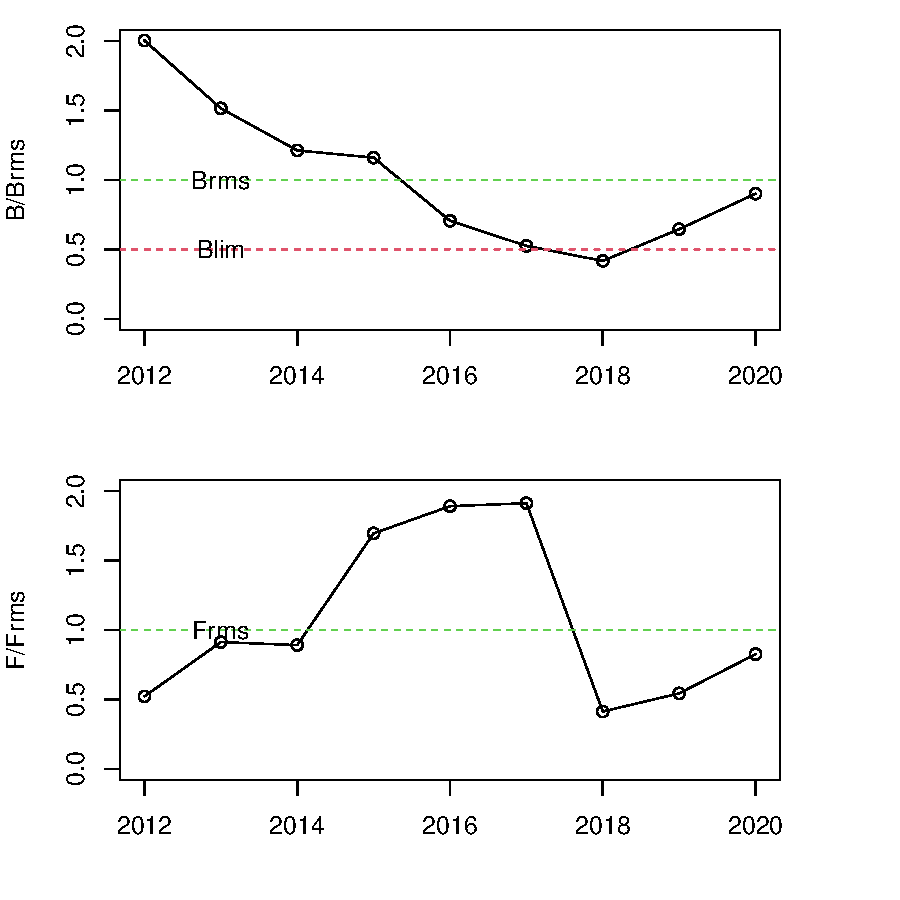
\includegraphics[width=0.8\textwidth]{Figuras/Fig11_InformeFinal-1.pdf}
\caption{Series históricas de la razón $B/B_{RMS}$ y $F/F_{RMS}$, estimadas en la asesoría de septiembre 2020 y junio 2021. Se muestran los puntos biológicos de referencia respectivos en líneas segmentadas horizontales.}
\label{Fig14}
\end{figure}

\pagebreak

\begin{figure}[h!]
\centering
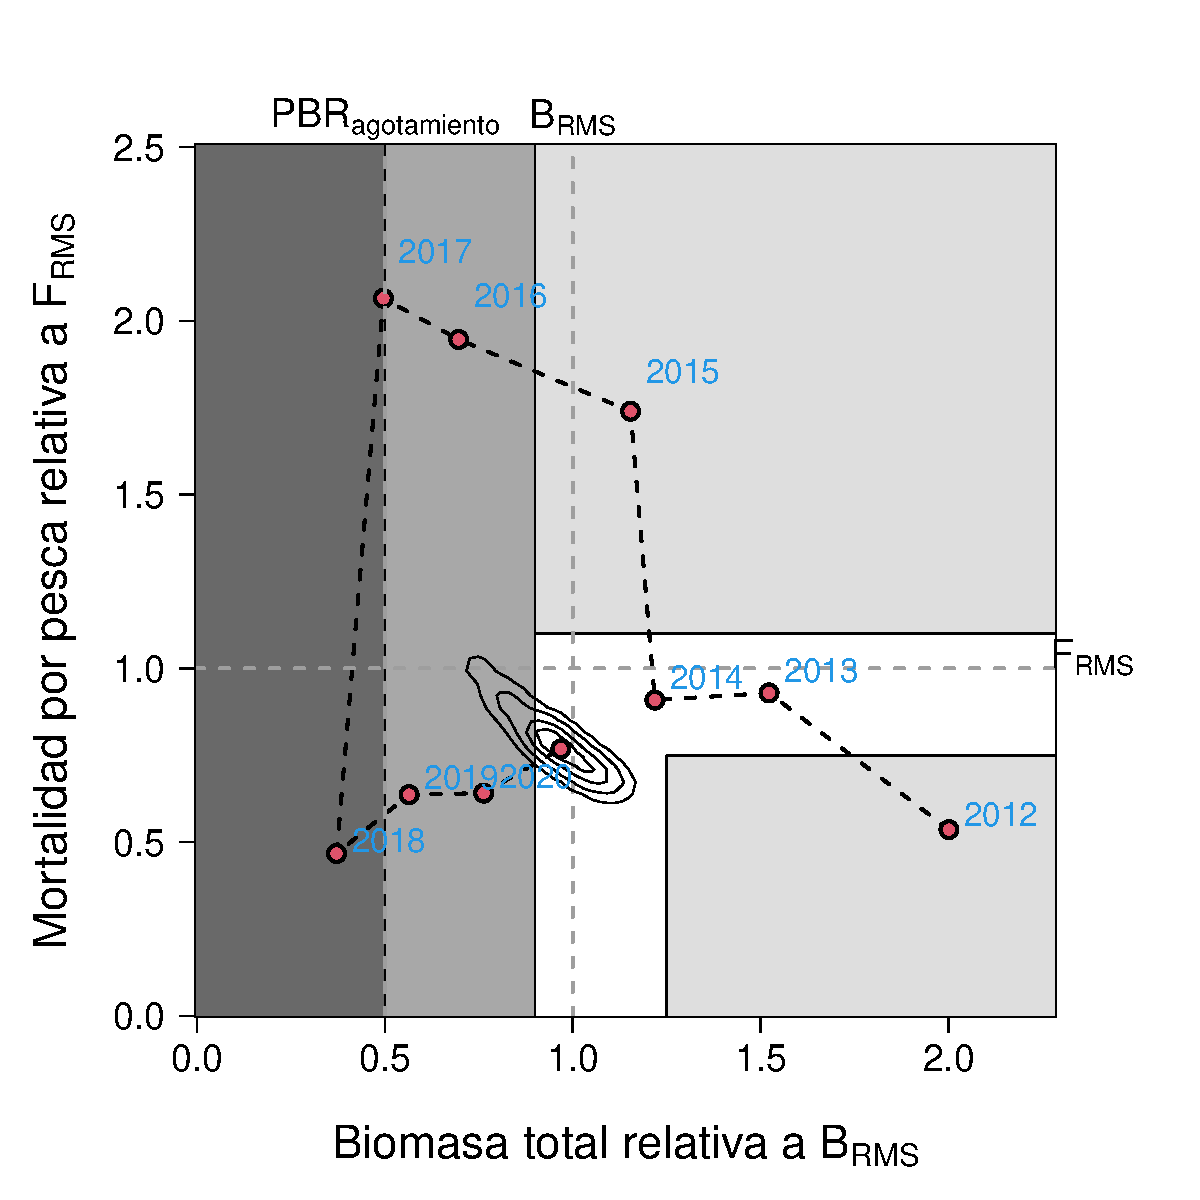
\includegraphics[width=0.9\textwidth]{Figuras/Fig4_Zhou2013_fase-1.pdf}
\caption{Diagrama de fase de sardina austral en la Región de Aysén. Las líneas verticales segmentadas indican los PBR al máximo rendimiento sostenido y aquel que indica el límite o colapso. La línea segmentada horizontal indica la mortalidad por pesca que permite el máximo rendimiento sostenido. Se muestra también la incertidumbre asociada al último año de la evaluación.}
\label{Fig15}
\end{figure}

\pagebreak

\hypertarget{objetivo-especuxedfico-3-1}{%
\subsection{4.3. Objetivo específico
3:}\label{objetivo-especuxedfico-3-1}}

\vspace{-0.2cm}

\emph{``Determinar niveles de Captura Biológicamente Aceptable (CBA) que
lleven y/o mantenga la pesquería en torno al Rendimiento Máximo
Sostenible (RMS), a partir de un análisis de riesgo en condiciones de
incertidumbre de no alcanzar los objetivos de conservación y
sostenibilidad conforme lo establece la LGPA y contenidos en el Plan de
Manejo y/o en el Programa de Recuperación respectivo, según
corresponda.''} \vspace{0.5cm}

\hypertarget{captura-bioluxf3gicamente-aceptable-cba-inicial-2021}{%
\subsubsection{4.3.1. Captura Biológicamente Aceptable (CBA) inicial
2021}\label{captura-bioluxf3gicamente-aceptable-cba-inicial-2021}}

A partir del modelo conceptual de la dinámica del stock de sardina
austral en aguas interiores Chiloé, se desarrolló el enfoque y modelo de
evaluación que permite asesorar al Comité Científico Técnico de
Pesquerías de Pelágicos Pequeños (CCT--PP) en el análisis de las
posibilidades de explotación del stock, considerando los parámetros e
indicadores estimados por el modelo de evaluación y su incertidumbre
asociada.

Se utiliza la estrategia de explotación referencial de mortalidad por
pesca constantes \(F=F_{RMS}\) para la cual se presentaron las capturas
asociadas y los percentiles de riesgo (10\%-50\%) de exceder el nivel de
explotación evaluado. La mortalidad por pesca de referencia es aquella
que permite alcanzar el rendimiento máximo sostenido, consistente con
los puntos biológicos de referencia (\(F_{RMS}\)).

La CBA se lleva a cabo bajo un vector de valores (0,67; 1,00; 1,25)
multiplicadores del \(F_{RMS}\), cuyo segundo valor del vector
corresponde al \(F_{RMS}\). Se realiza una proyección del stock al año
2021 para estimar la CBA inicial.

En la \textbf{Tabla \ref{Tab11}} se resumen los distintos niveles de
capturas de sardina austral para la Región de Aysén durante el año 2021.
Las estrategias que llevan a la biomasa a la \(B_{RMS}\) en el corto
plazo sugieren para el año 2021 un nivel de captura del orden de las 4,2
mil toneladas para un nivel de mortalidad por pesca igual al \(F_{RMS}\)
(0,46 año\textsuperscript{-1}). Niveles de captura más conservadores,
por ejemplo, con F0,67*\(F_{RMS}\). (0,31 año\textsuperscript{-1})
serían del orden de las 2,8 mil toneladas.

\vspace{0.5cm}

\begin{longtable}[]{@{}cccc@{}}
\caption{\label{Tab11} Captura biológicamente aceptable de sardina
austral en la Región de Aysén para el año 2021 para distintos niveles de
mortalidad por pesca y bajo diferentes percentiles de captura al
RMS.}\tabularnewline
\toprule
\begin{minipage}[b]{0.17\columnwidth}\centering
Percentiles\strut
\end{minipage} & \begin{minipage}[b]{0.14\columnwidth}\centering
F = 0,31\strut
\end{minipage} & \begin{minipage}[b]{0.14\columnwidth}\centering
F = 0,46\strut
\end{minipage} & \begin{minipage}[b]{0.14\columnwidth}\centering
F = 0,58\strut
\end{minipage}\tabularnewline
\midrule
\endfirsthead
\toprule
\begin{minipage}[b]{0.17\columnwidth}\centering
Percentiles\strut
\end{minipage} & \begin{minipage}[b]{0.14\columnwidth}\centering
F = 0,31\strut
\end{minipage} & \begin{minipage}[b]{0.14\columnwidth}\centering
F = 0,46\strut
\end{minipage} & \begin{minipage}[b]{0.14\columnwidth}\centering
F = 0,58\strut
\end{minipage}\tabularnewline
\midrule
\endhead
\begin{minipage}[t]{0.17\columnwidth}\centering
10\%\strut
\end{minipage} & \begin{minipage}[t]{0.14\columnwidth}\centering
2.770\strut
\end{minipage} & \begin{minipage}[t]{0.14\columnwidth}\centering
4.155\strut
\end{minipage} & \begin{minipage}[t]{0.14\columnwidth}\centering
5.193\strut
\end{minipage}\tabularnewline
\begin{minipage}[t]{0.17\columnwidth}\centering
20\%\strut
\end{minipage} & \begin{minipage}[t]{0.14\columnwidth}\centering
2.779\strut
\end{minipage} & \begin{minipage}[t]{0.14\columnwidth}\centering
4.169\strut
\end{minipage} & \begin{minipage}[t]{0.14\columnwidth}\centering
5.211\strut
\end{minipage}\tabularnewline
\begin{minipage}[t]{0.17\columnwidth}\centering
30\%\strut
\end{minipage} & \begin{minipage}[t]{0.14\columnwidth}\centering
2.786\strut
\end{minipage} & \begin{minipage}[t]{0.14\columnwidth}\centering
4.179\strut
\end{minipage} & \begin{minipage}[t]{0.14\columnwidth}\centering
5.223\strut
\end{minipage}\tabularnewline
\begin{minipage}[t]{0.17\columnwidth}\centering
40\%\strut
\end{minipage} & \begin{minipage}[t]{0.14\columnwidth}\centering
2.791\strut
\end{minipage} & \begin{minipage}[t]{0.14\columnwidth}\centering
4.186\strut
\end{minipage} & \begin{minipage}[t]{0.14\columnwidth}\centering
5.233\strut
\end{minipage}\tabularnewline
\begin{minipage}[t]{0.17\columnwidth}\centering
50\%\strut
\end{minipage} & \begin{minipage}[t]{0.14\columnwidth}\centering
2.797\strut
\end{minipage} & \begin{minipage}[t]{0.14\columnwidth}\centering
4.196\strut
\end{minipage} & \begin{minipage}[t]{0.14\columnwidth}\centering
5.245\strut
\end{minipage}\tabularnewline
\bottomrule
\end{longtable}

\normalsize

\pagebreak

\hypertarget{captura-bioluxf3gicamente-aceptable-cba-2021}{%
\subsubsection{4.3.2. Captura Biológicamente Aceptable (CBA)
2021}\label{captura-bioluxf3gicamente-aceptable-cba-2021}}

A partir del modelo conceptual de la dinámica del stock de sardina
austral en aguas interiores Chiloé, se desarrolló el enfoque y modelo de
evaluación que permite asesorar al Comité Científico Técnico de
Pesquerías de Pelágicos Pequeños (CCT--PP) en el análisis de las
posibilidades de explotación del stock, considerando los parámetros e
indicadores estimados por el modelo de evaluación y su incertidumbre
asociada.

Se utiliza la estrategia de explotación referencial de mortalidad por
pesca constantes \(F=F_{RMS}\) para la cual se presentaron las capturas
asociadas y los percentiles de riesgo (10\%-50\%) de exceder el nivel de
explotación evaluado. La mortalidad por pesca de referencia es aquella
que permite alcanzar el rendimiento máximo sostenido, consistente con
los puntos biológicos de referencia (\(F_{RMS}\)).

La CBA se lleva a cabo bajo un vector de valores (0,67; 1,00; 1,25)
multiplicadores del \(F_{RMS}\), cuyo segundo valor del vector
corresponde al \(F_{RMS}\). Se realiza una proyección del stock al año
2021 para estimar la CBA actualizada.

En la \textbf{Tabla \ref{Tab12}} se resumen los distintos niveles de
capturas de sardina austral para la Región de Aysén durante el año 2021.
Las estrategias que llevan a la biomasa a la \(B_{RMS}\) en el corto
plazo sugieren para el año 2021 un nivel de captura del orden de las 4,6
mil toneladas para un nivel de mortalidad por pesca igual al \(F_{RMS}\)
(0,46 año\textsuperscript{-1}). Niveles de captura más conservadores,
por ejemplo, con F0,67*\(F_{RMS}\). (0,31 año\textsuperscript{-1})
serían del orden de las 3,1 mil toneladas.

\vspace{0.5cm}

\begin{longtable}[]{@{}llll@{}}
\caption{\label{Tab12} Captura biológicamente aceptable de sardina
austral en la Región de Aysén para el año 2021 para distintos niveles de
mortalidad por pesca y bajo diferentes percentiles de captura al
RMS.}\tabularnewline
\toprule
\begin{minipage}[b]{0.17\columnwidth}\raggedright
Percentiles\strut
\end{minipage} & \begin{minipage}[b]{0.14\columnwidth}\raggedright
F = 0,31\strut
\end{minipage} & \begin{minipage}[b]{0.14\columnwidth}\raggedright
F = 0,46\strut
\end{minipage} & \begin{minipage}[b]{0.14\columnwidth}\raggedright
F = 0,58\strut
\end{minipage}\tabularnewline
\midrule
\endfirsthead
\toprule
\begin{minipage}[b]{0.17\columnwidth}\raggedright
Percentiles\strut
\end{minipage} & \begin{minipage}[b]{0.14\columnwidth}\raggedright
F = 0,31\strut
\end{minipage} & \begin{minipage}[b]{0.14\columnwidth}\raggedright
F = 0,46\strut
\end{minipage} & \begin{minipage}[b]{0.14\columnwidth}\raggedright
F = 0,58\strut
\end{minipage}\tabularnewline
\midrule
\endhead
\begin{minipage}[t]{0.17\columnwidth}\raggedright
10\%\strut
\end{minipage} & \begin{minipage}[t]{0.14\columnwidth}\raggedright
3.081\strut
\end{minipage} & \begin{minipage}[t]{0.14\columnwidth}\raggedright
4.621\strut
\end{minipage} & \begin{minipage}[t]{0.14\columnwidth}\raggedright
5.776\strut
\end{minipage}\tabularnewline
\begin{minipage}[t]{0.17\columnwidth}\raggedright
20\%\strut
\end{minipage} & \begin{minipage}[t]{0.14\columnwidth}\raggedright
3.088\strut
\end{minipage} & \begin{minipage}[t]{0.14\columnwidth}\raggedright
4.632\strut
\end{minipage} & \begin{minipage}[t]{0.14\columnwidth}\raggedright
5.790\strut
\end{minipage}\tabularnewline
\begin{minipage}[t]{0.17\columnwidth}\raggedright
30\%\strut
\end{minipage} & \begin{minipage}[t]{0.14\columnwidth}\raggedright
3.098\strut
\end{minipage} & \begin{minipage}[t]{0.14\columnwidth}\raggedright
4.647\strut
\end{minipage} & \begin{minipage}[t]{0.14\columnwidth}\raggedright
5.808\strut
\end{minipage}\tabularnewline
\begin{minipage}[t]{0.17\columnwidth}\raggedright
40\%\strut
\end{minipage} & \begin{minipage}[t]{0.14\columnwidth}\raggedright
3.104\strut
\end{minipage} & \begin{minipage}[t]{0.14\columnwidth}\raggedright
4.655\strut
\end{minipage} & \begin{minipage}[t]{0.14\columnwidth}\raggedright
5.819\strut
\end{minipage}\tabularnewline
\begin{minipage}[t]{0.17\columnwidth}\raggedright
50\%\strut
\end{minipage} & \begin{minipage}[t]{0.14\columnwidth}\raggedright
3.109\strut
\end{minipage} & \begin{minipage}[t]{0.14\columnwidth}\raggedright
4.663\strut
\end{minipage} & \begin{minipage}[t]{0.14\columnwidth}\raggedright
5.829\strut
\end{minipage}\tabularnewline
\bottomrule
\end{longtable}

\normalsize

\pagebreak

\hypertarget{proyecciuxf3n-del-stock}{%
\subsubsection{4.3.3. Proyección del
stock}\label{proyecciuxf3n-del-stock}}

La \textbf{Figura \ref{Fig16}} muestra las proyecciones de la biomasa de
sardina austral en aguas interiores de la Región de Aysén. Se observa
que la mortalidad por pesca igual al \(F_{RMS}\) (\(F_{RMS}\)=0,46
año\textsuperscript{-1}), permitiría llevar la biomasa en un nivel
cercano y por sobre al punto biológico de referencia (\(B_{RMS}\)). En
cambio, para aquel valor de mortalidad por pesca superior (0,58
año\textsuperscript{-1}) al \(F_{RMS}\) mantienen la biomasa por debajo
del rendimiento máximo sostenido.

\vspace{0.5cm}

\begin{figure}[h!]
\centering
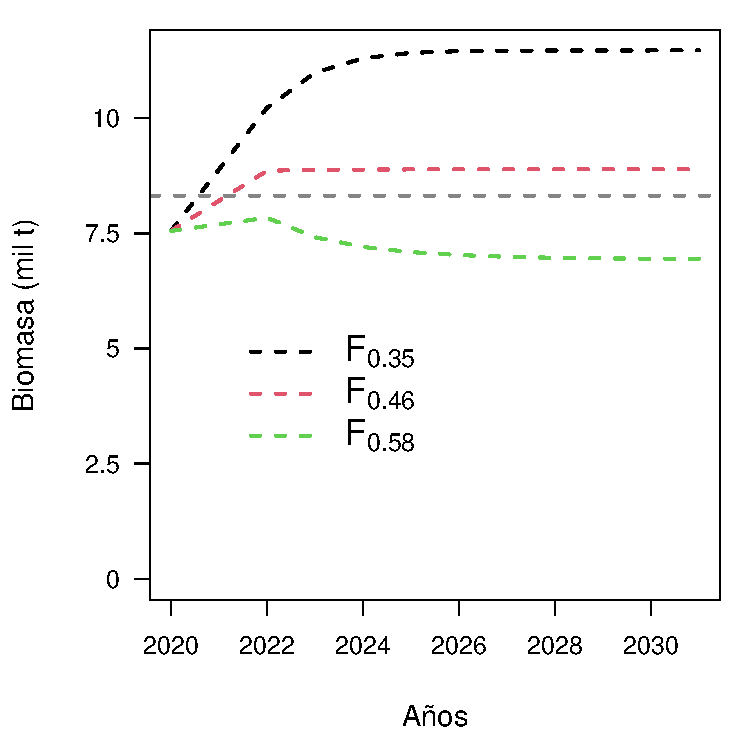
\includegraphics[width=0.5\textwidth]{Figuras/Fig5_Zhou2013_Proyeccion_B-1.pdf}
\end{figure}

\vspace{-0.1cm}

\begin{figure}[h!]
\centering
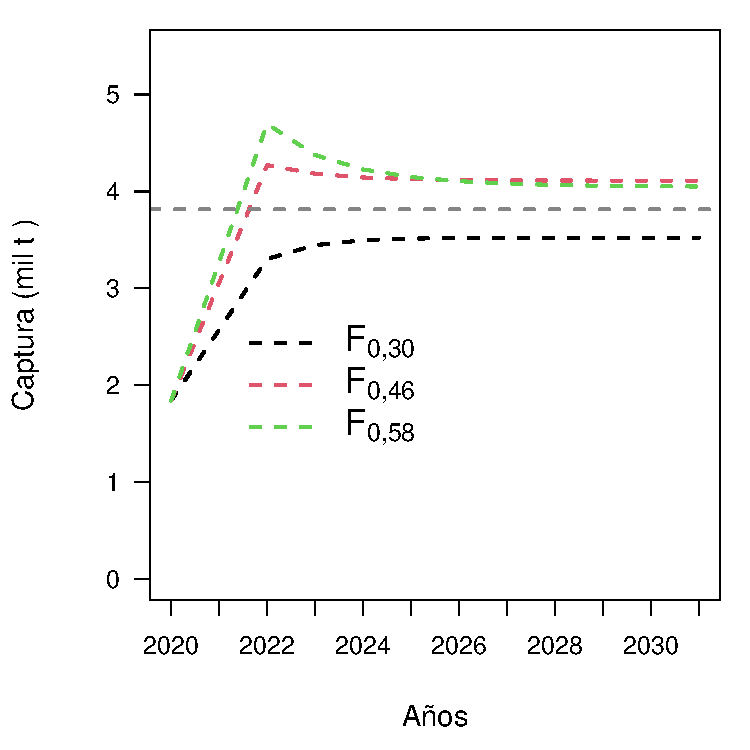
\includegraphics[width=0.5\textwidth]{Figuras/Fig6_Zhou2013_capturas-1.pdf}
\caption{Proyecciones de la biomasa de sardina austral (panel superior) y captura de sardina austral (panel inferior) en aguas interiores de la Región de Aysén con diferentes valores de mortalidad por pesca. La línea punteada horizontal gris representa biomasa al máximo rendimiento sostenible ($B_{RMS}$) y el máximo rendimiento sostenible ($RMS$).}
\label{Fig16}
\end{figure}

\pagebreak

\hypertarget{objetivo-especuxedfico-4-1}{%
\subsection{4.4. Objetivo específico
4:}\label{objetivo-especuxedfico-4-1}}

\vspace{-0.2cm}

\emph{``Informar el avance del Programa de Mejoramiento Continuo de la
Calidad en la Asesoría Científica (PMCCAC) realizado durante el presente
estudio, respecto al cumplimiento de recomendaciones formuladas en
procesos de RPEI y priorizadas por el CCT, cuando corresponda.''}
\vspace{0.5cm}

\hypertarget{esquema-de-trabajo-y-plan-de-actividades-2019-2021}{%
\subsubsection{4.4.1. Esquema de trabajo y plan de actividades
2019-2021}\label{esquema-de-trabajo-y-plan-de-actividades-2019-2021}}

En coherencia con los requerimientos indicados en los Términos Técnicos
de Referencia (TTR) del proyecto ``Estatus y posibilidades de
explotación biológicamente sustentables de los principales recursos
pesqueros nacionales'', IFOP ha reconocido un conjunto de actividades
que pueden ser desarrolladas y abordadas bajo un acuerdo de intención
con SSPA. Además de los correspondientes informes técnicos, se han
identificado una serie de aspectos a ser abordados en el marco de la
evaluación de stock. Estos aspectos son de carácter transversal a los
recursos pelágicos analizados y otros particulares en la evaluación de
stock de la sardina austral. Para ello se propone el esquema de trabajo
presentado en la \textbf{Figura \ref{Fig17}}, el cual fue discutido y
consensuado con la SSPA.

\vspace{0.5cm}

\begin{figure}[h!]
\centering
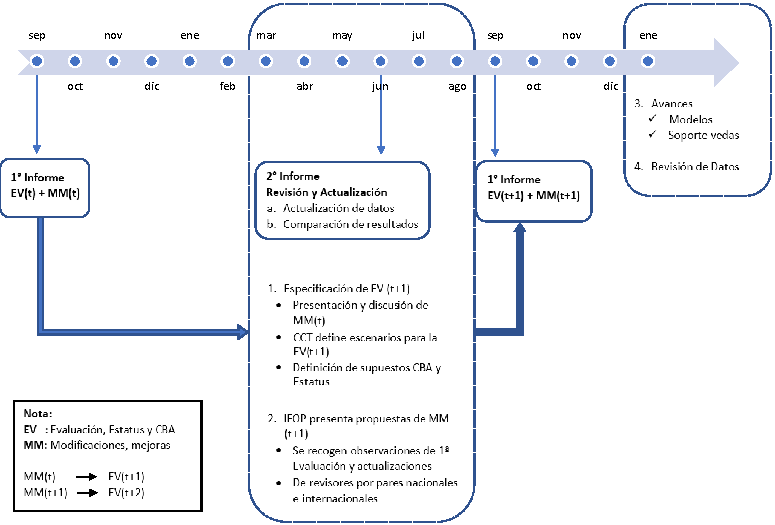
\includegraphics[width=1\textwidth]{Figuras/EsquemaTrabajo.pdf}
\caption{Esquema de trabajo de Datos y Modelos propuesto por SSPA e IFOP para la implementación de mejoras y modificaciones (MM) a la evaluación de stock (EV) durante el desarrollo del Proyecto de Estatus y CBA de las pesquerías de Pelágicos.}
\label{Fig17}
\end{figure}

\vspace{0.5cm}

El esquema de trabajo de datos y modelos consiste en los siguientes
pasos:

\begin{enumerate}
\def\labelenumi{\roman{enumi})}
\item
  Especificación de EV(t+1) (septiembre) sobre la base de las MM(t)
  presentadas en la asesoría anterior, EV(t) las cuales serán
  presentadas y discutidas con el CCT-PP para la definición del caso
  base, EV(t+1), utilizado para establecer el estatus y CBA.
\item
  IFOP presenta propuestas de MM(t+1) para trabajar durante el
  desarrollo de este proyecto que recogerán algunas de las observaciones
  a la EV(t) de revisores por pares (RPP) nacionales, CCT-PP y SSPA,
  junto a recomendaciones de la RPP internacional.
\item
  Uno de los propósitos de este esquema de trabajo es que en esta
  instancia también se realice la revisión de datos, sin embargo, en
  este proyecto en particular se dará prioridad a la propuesta de
  MM(t+1), con el compromiso que la revisión de datos se lleve a cabo en
  los futuros proyectos.
\item
  En la etapa de revisión y actualización de la EV(t+2) a realizarse en
  junio de 2020, también se comparará con los resultados de la EV(t+1)
  correspondiente a la asesoría de septiembre 2019.
\item
  Finalmente, es importante señalar que la evaluación de stock del
  recurso es realizada separada por zonas: Los Lagos y Aysén en
  coherencia con los antecedentes de stock diferenciados. La
  actualización de la evaluación de stock EV(t+2) ha tenidos en los
  últimos dos años retrasos en la fecha comprometida debido a
  dificultades operativas del crucero de evaluación directa (principal
  input para la actualización). Se plantea entonces, comprometer una
  fecha para la entrega del informe de actualización, con mayor
  flexibilidad y dependiente de la entrega de los resultados del
  crucero.
\end{enumerate}

\vspace{0.5cm}

\hypertarget{resultados-preliminares-de-la-implementaciuxf3n-de-muxe9todos-alternativos-para-determinaciuxf3n-de-estatus-en-sardina-austral-de-la-regiuxf3n-de-aysuxe9n.}{%
\subsubsection{4.4.2. Resultados preliminares de la implementación de
métodos alternativos para determinación de Estatus en sardina austral de
la Región de
Aysén.}\label{resultados-preliminares-de-la-implementaciuxf3n-de-muxe9todos-alternativos-para-determinaciuxf3n-de-estatus-en-sardina-austral-de-la-regiuxf3n-de-aysuxe9n.}}

\vspace{0.5cm}

\hypertarget{a-spict-stochastic-surplus-production-model-in-continuous-time-peteresen-berg-2017-1}{%
\paragraph{a) SPiCT, Stochastic Surplus Production Model in Continuous
Time (Peteresen \& Berg,
2017)}\label{a-spict-stochastic-surplus-production-model-in-continuous-time-peteresen-berg-2017-1}}

\quad

El período de análisis abarca los años 2006 a 2020. Los índices que se
utilizan en este modelo, corresponden a la información de desembarques
oficiales (Sernapesca) y biomasa del crucero (\(B_{cru}\)) de evaluación
directa desarrollado por IFOP en aguas interiores de la Región de Aysén
(\textbf{Figura \ref{Fig18}}).

\begin{figure}[h!]
\centering
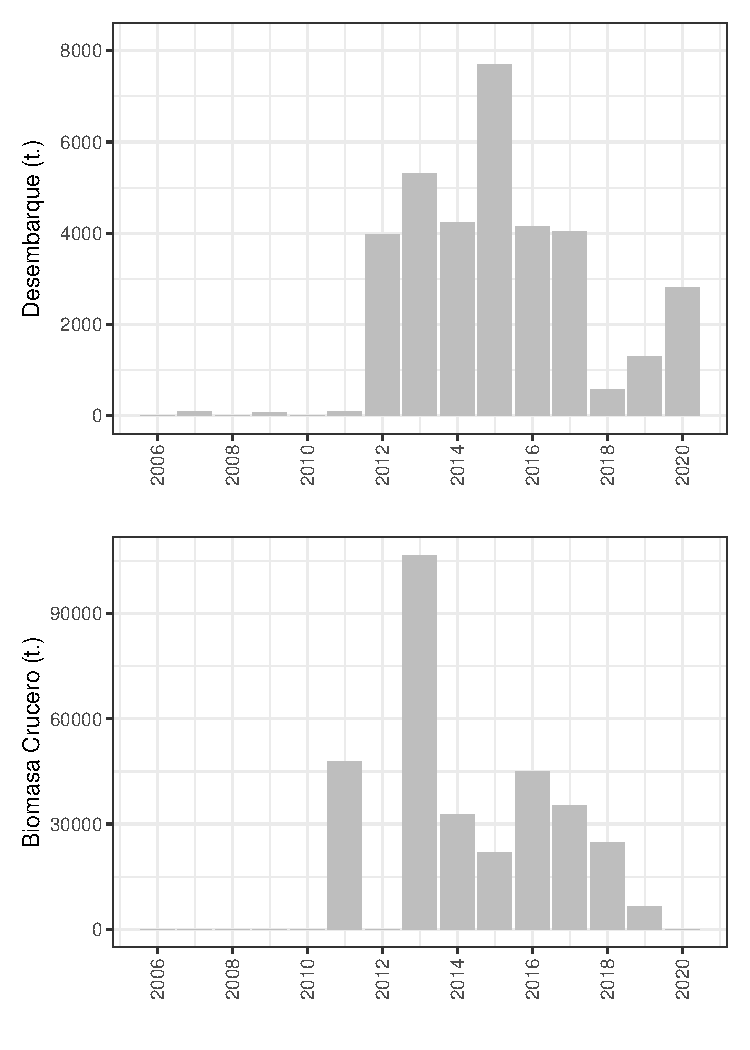
\includegraphics[width=0.5\textwidth]{SPiCT/Figuras/datos-1.pdf}
\caption{Ajuste a la estructura de tallas de las capturas de sardina austral de la Región de Aysén.}
\label{Fig18}
\end{figure}

\pagebreak

La \textbf{Tabla \ref{Tab13}} muestra las estimaciones de los parámetros
del modelo con Intervalos de confianza del 95\% para el modelo de
producción excedentaria. Hay que tener en cuenta que el intervalo de
confianza para el parámetro de forma de producción \(n\) incluye el
simétrico (Schaefer) caso n = 2. De este modelo t, no podemos decir con
certeza si la producción de biomasa está sesgada. La capacidad de carga
para el stock explotable se prevé que sea aproximadamente 10.02 mil t.
para la curva de producción general. Sin embargo, el intervalo de
dependencia es extremadamente amplio con un intervalo más bajo de 4300
t. y un intervalo superior de 135 mil t. Claramente, las predicciones
del modelo están sufriendo debido a la escasez de datos y quizas a una
basica sintonización del modelo. Sin embargo, el modelo proporciona una
primera estimación de la abundancia absoluta. Con respecto a las
variables de estado calculadas consideran un nivel de biomasas para el
ultimo año de mil toneladas aproximadamente. \vspace{0.5cm}

\small

\begin{longtable}[]{@{}llll@{}}
\caption{\label{Tab13} Parámetros estimados del modelo IC 95\%,
estimación determinista de puntos de referencia y estimación stocástica
de puntos de referencia. \normalsize}\tabularnewline
\toprule
parámetros & estimado & IC inferior & IC superior\tabularnewline
\midrule
\endfirsthead
\toprule
parámetros & estimado & IC inferior & IC superior\tabularnewline
\midrule
\endhead
alpha & 2,00 & 2,00 & 2,00\tabularnewline
beta & 2,00 & 2,00 & 2,00\tabularnewline
n & 12 & 11,98 & 12,02\tabularnewline
r & 6,57 & 1,90 & 22,77\tabularnewline
K & 10.021 & 2.302 & 43.617\tabularnewline
------------ & -------------- & ------------- &
-------------\tabularnewline
Parámetros & Determinista & IC inferior & IC superior\tabularnewline
------------ & -------------- & ------------- &
-------------\tabularnewline
Bmsy & 7.994 & 1.837 & 34.797\tabularnewline
Fmsy & 0,55 & 0,16 & 1,90\tabularnewline
MSY & 4.380 & 1.184 & 16.201\tabularnewline
------------ & -------------- & ------------- &
-------------\tabularnewline
Parámetros & Estocástico & IC inferior & IC superior\tabularnewline
------------ & -------------- & --------------- &
-------------\tabularnewline
Bmsy & 6.235 & 1.175 & 33.072\tabularnewline
Fmsy & 0,39 & 0,06 & 2,46\tabularnewline
MSY & 2.133 & 365 & 12.475\tabularnewline
\bottomrule
\end{longtable}

\normalsize

La \textbf{Figura \ref{Fig19}} muestra la biomasa absoluta del stock de
sardina austral para la Region de Aysén un declive desde el año 2015
cercano a las mil t., pero con un alto grado de incertidumbre de
estimación. De la misma manera, el gráfico superior izquierdo muestra un
progresivo aumento de la mortalidad por pesca relativa a un eventual
objetivo de manejo (\(F_{RMS}\)). También es posible identificar la
trayectoria de la mortalidad por pesca absoluta, que están por sobre un
eventual PBR del RMS indicado en la línea negra. Además, se estima para
el año 2020 un F en 1.71 año\textsuperscript{-1}. Amplios intervalos de
confianza como lo indica la zona sombreada de los gráficos para los
parámetros estimados y la serie de tiempo de biomasa del proceso de
ajuste y sintonización del modelo de evaluación utilizado. El grafico
inferior derecho se identifica la curva de producción de la población,
en donde es posible identificar que el año 2018 el stock de sardina
austral estuvo en su maximo rendimiento a través de la remoción del
excedente.

La \textbf{Figura \ref{Fig20}} muestra la evolución de la biomasa y la
mortalidad por pesca desde el año inicial (aquí 2006) indicado con un
círculo hasta el año terminal (aquí 2020) indicado con un cuadrado en un
esquema de fases. El diamante amarillo indica la biomasa media durante
un largo período si se mantiene la presión pesquera actual (2020). Este
punto se puede interpretar como el equilibrio de captura y se denota E
(Bo) en la leyenda de la figura como una forma estadística de expresar
la expectativa de la biomasa como t=o.

De acuerdo a este diagrama, la pesquería de sardina austral estuvo
sometida a bajos niveles de presión pesquera en los primeros años
analizados años, por lo cual su estado representado por el diagrama de
fase se encuentra en niveles subexplotados. En los años recientes esta
situación cambia para pasar a una fase de sobrepesca y sobre
explotación. Una línea roja discontinua vertical en Bt = 0 indica el
nivel de biomasa por debajo del cual la población se ha desplomado. Esta
pesquería comienza en un estado de vulnerabilidad el año 2006. Es
importante visualizarlos conjuntamente ya que los dos puntos de
referencia están altamente (negativamente) correlacionados.

\begin{figure}[h!]
\centering
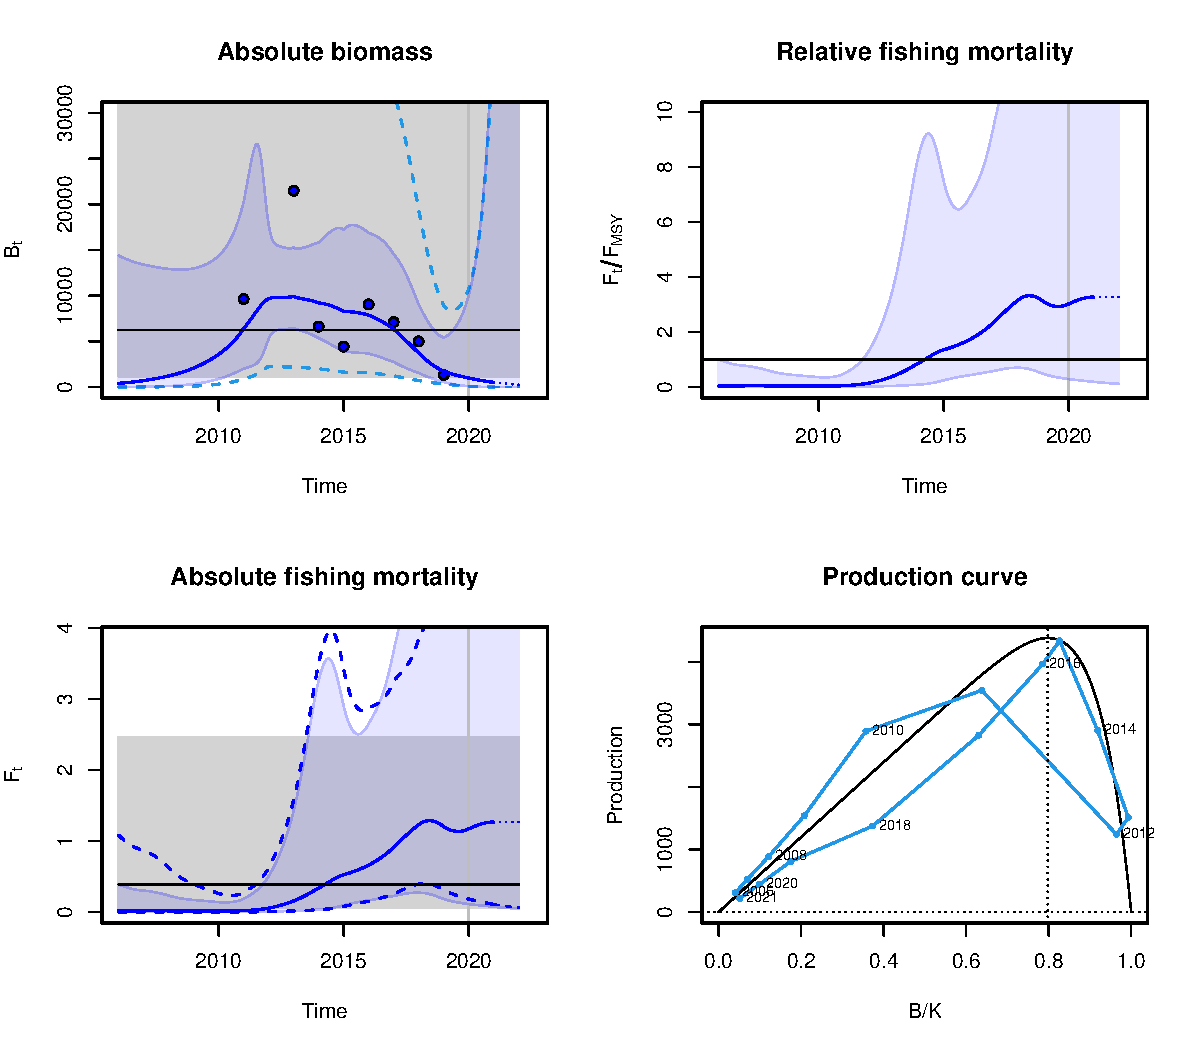
\includegraphics[width=0.9\textwidth]{SPiCT/Figuras/Salidas-1.pdf}
\caption{Estimaciones SPiCT estimado en sardina austral de (a) la biomasa absoluta, (b) mortalidad por pesca relativa, (c)  mortalidad por pesca absoluta y (d)  curvas de producción derivadas del modelo. Las líneas (azules) indican valores medianos y áreas sombreadas en indicar intervalos de confianza (IC) del 95\%. Líneas negras horizontales denotan PBR de la pesquería.}
\label{Fig19}
\end{figure}

\pagebreak

\begin{figure}[h!]
\centering
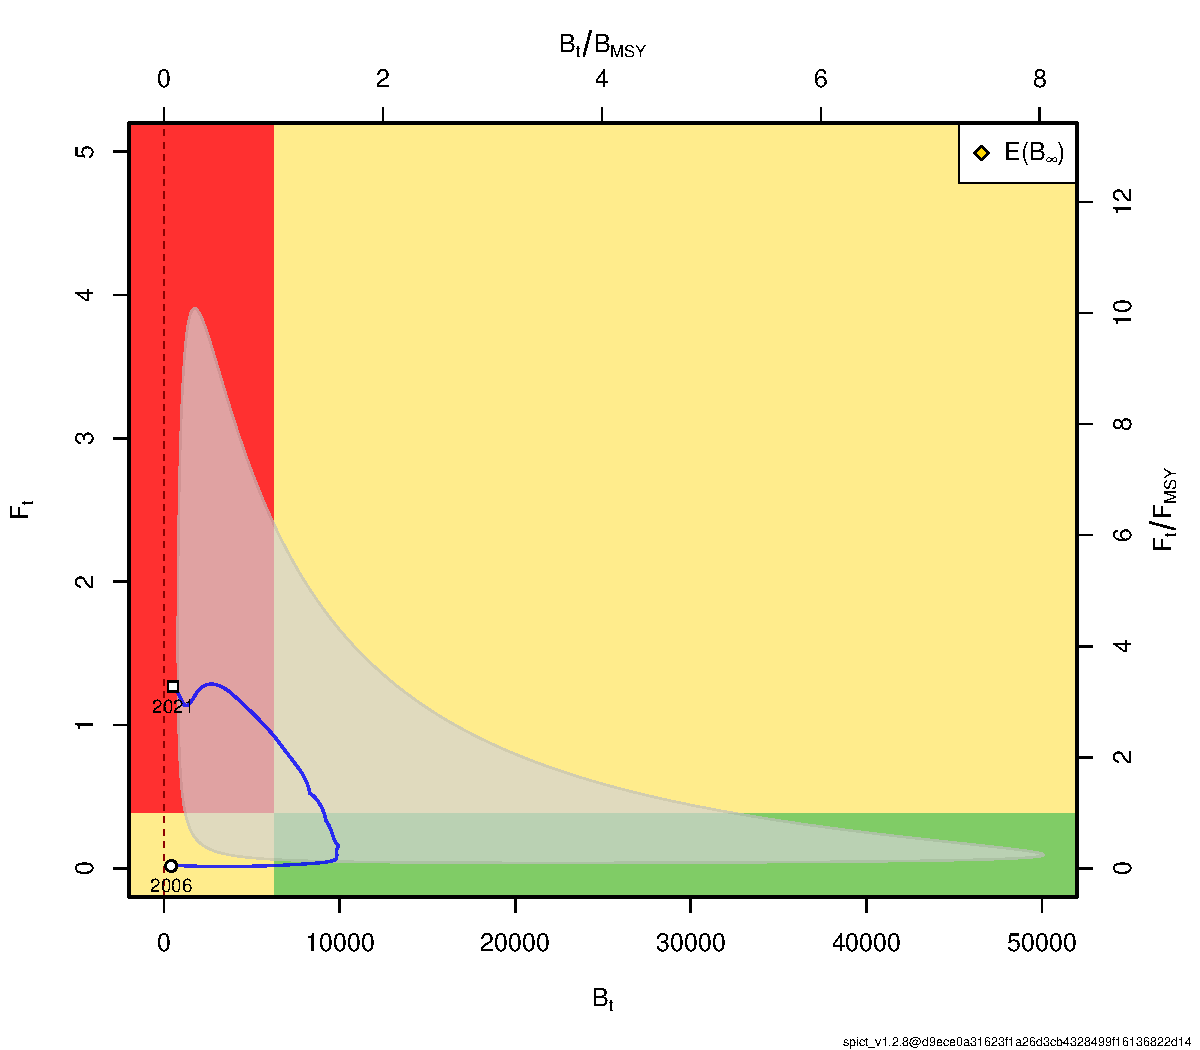
\includegraphics[width=0.9\textwidth]{SPiCT/Figuras/Salidas 2-1.pdf}
\caption{Diagrama de explotación B-F de sardina austral Región de Aysén durante los años 2006 y 2020.}
\label{Fig20}
\end{figure}

\pagebreak

\hypertarget{b-lbpa-length-based-pseudocohort-analysis-canales-et-al.-2020-1}{%
\paragraph{\texorpdfstring{b) LBPA, Length-Based Pseudocohort Analysis
(Canales \emph{et al}.,
2020)}{b) LBPA, Length-Based Pseudocohort Analysis (Canales et al., 2020)}}\label{b-lbpa-length-based-pseudocohort-analysis-canales-et-al.-2020-1}}

\quad

La \textbf{Tabla \ref{Tab14}} muestra los parámetros biológicos de
sardina austral utilizados en el análisis de pseudocohortes basado en
estructuras de tallas. La \textbf{Figura \ref{Fig21}} muestra el ajuste
a la estructura de tallas de las capturas de la flota que opera sobre el
stock de sardina austral de la Región de Aysén, el cual logra
representar la bimodalidad típica que se observa en estructuras de
tallas de peces pelágicos, pero aún con dificultades para representar
las modas intermedias (\textbf{Figura \ref{Fig22}}). En general se
observa una baja proporción de individuos adultos sobre los 15 cm LT y
una alta proporción de reclutas. El método LBPA tiene como objetivo
generar a través de simulaciones las estructuras de tallas que no han
estado bajo efectos de la pesca y comparar estas con las estructuras de
tallas calculadas en función del SPR objetivo (SPR60\%). En la
\textbf{Figura \ref{Fig23}} se comparan la estructura de talla actual,
objetivo y sin pesca para evaluar el efecto de la pesquería sobre el
recurso. La selectividad estimada por el modelo indica que existe una
alta selección de individuos juveniles, bajo la talla media de madurez
(\textbf{Figura \ref{Fig24}}). La \textbf{Figura \ref{Fig25}} muestra la
curva de rendimiento por recluta (YPR) y la biomasa desovante por
recluta (SPR) del cual se obtiene los niveles de mortalidad por pesca
objetivo y actual para la pesquería de sardina austral de la Región de
Aysén. La \textbf{Figura \ref{Fig26}} muestra el diagrama de fase, donde
las líneas verticales representan el SPR objetivo (60\%SPRo) y SPR
límite y la línea horizontal representa la mortalidad por pesca objetivo
(F60\%SPR). Al respecto, dada la alta selectividad de individuos bajo la
talla de madurez y la baja proporción de individuos adultos, el estatus
esperado es sobrepesca y sobre-explotación. No obstante, cabe recordar
que los parámetros biológicos utilizados en este análisis corresponden a
estimaciones realizadas para sardina austral de la Región de Los Lagos,
por lo tanto, estas estimaciones se consideran preliminares hasta contar
con información biológica del stock de Aysén.

\vspace{0.5cm}

\begin{longtable}[]{@{}lll@{}}
\caption{\label{Tab14} Parámetros de crecimiento y mortalidad natural
.}\tabularnewline
\toprule
Parámetros & símbolo & valor fijo\tabularnewline
\midrule
\endfirsthead
\toprule
Parámetros & símbolo & valor fijo\tabularnewline
\midrule
\endhead
Longitud asintótica & Loo & 17,71\tabularnewline
Coeficiente crecimiento & k & 0,78\tabularnewline
Mortalidad natural & M & 0,84\tabularnewline
Relación longitud-peso & log\_a, b & -4,9636; 2,99\tabularnewline
Longitud de madurez & L50, L95 & 13,5 - 15 cm\tabularnewline
Período de desove & dt & 0,83\tabularnewline
Número de edades & n\_edad & 6 años\tabularnewline
\bottomrule
\end{longtable}

\begin{figure}[h!]
\centering
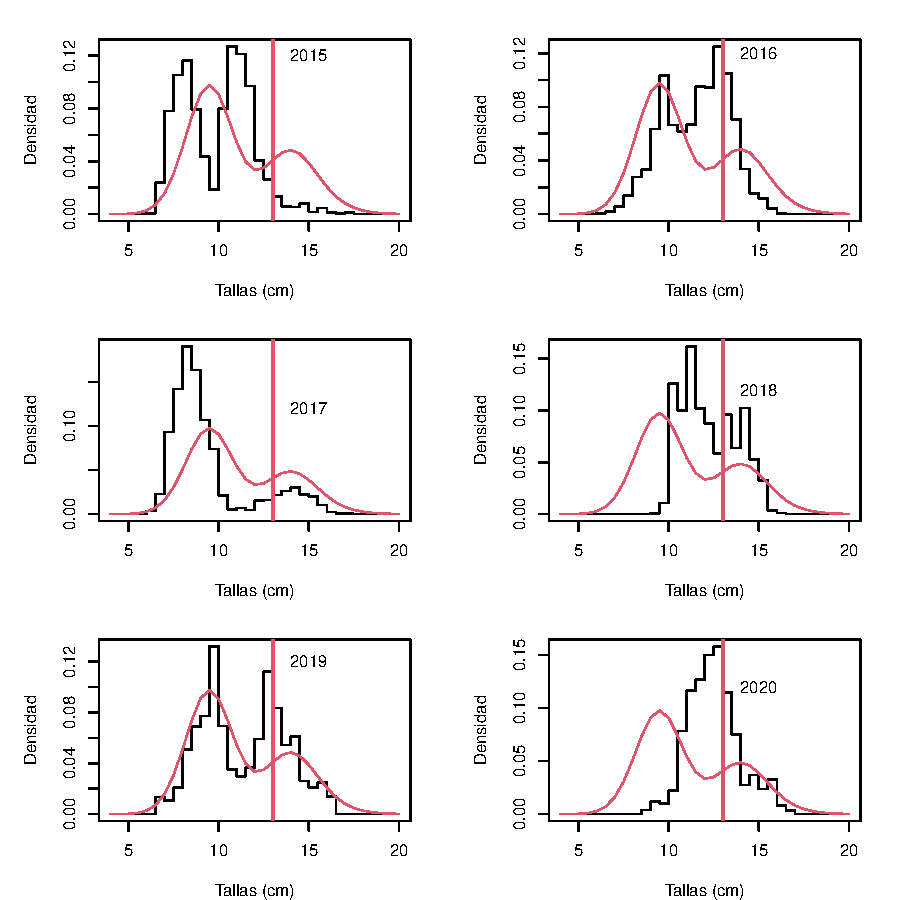
\includegraphics[width=0.7\textwidth]{LBPA/Figuras/ajuste_tallas-1.pdf}
\caption{Ajuste a la estructura de tallas de las capturas de sardina austral de la Región de Aysén.}
\label{Fig21}
\end{figure}

\begin{figure}[h!]
\centering
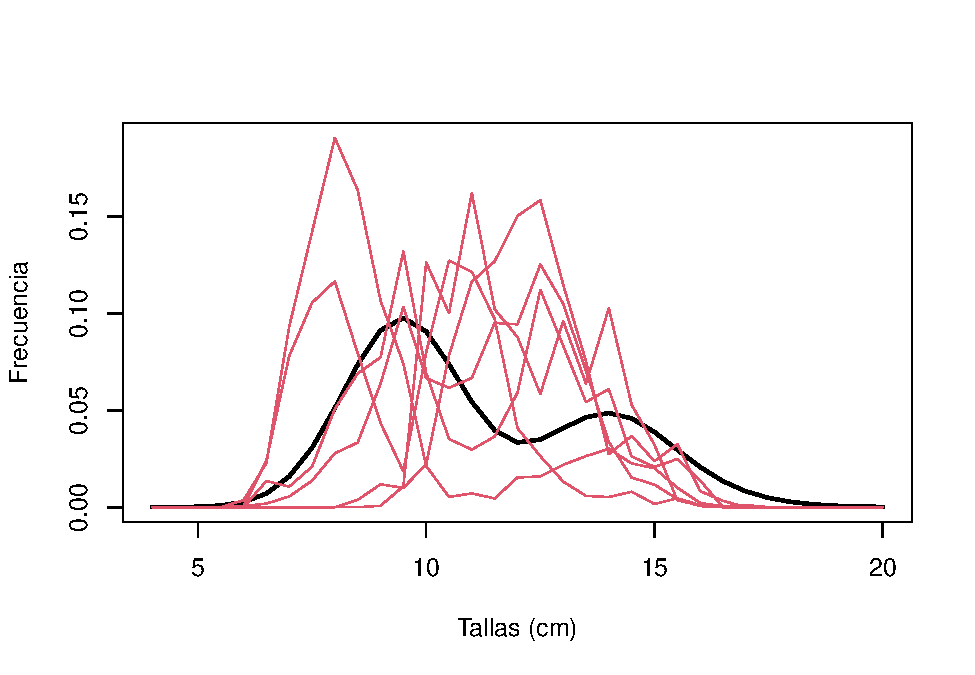
\includegraphics[width=0.7\textwidth]{LBPA/Figuras/ajusteTallasAcumuladas-1.pdf}
\caption{Ajuste a la estructura de tallas acumuladas de las capturas de sardina austral de la Región de Aysén.}
\label{Fig22}
\end{figure}

\pagebreak

\begin{figure}[h!]
\centering
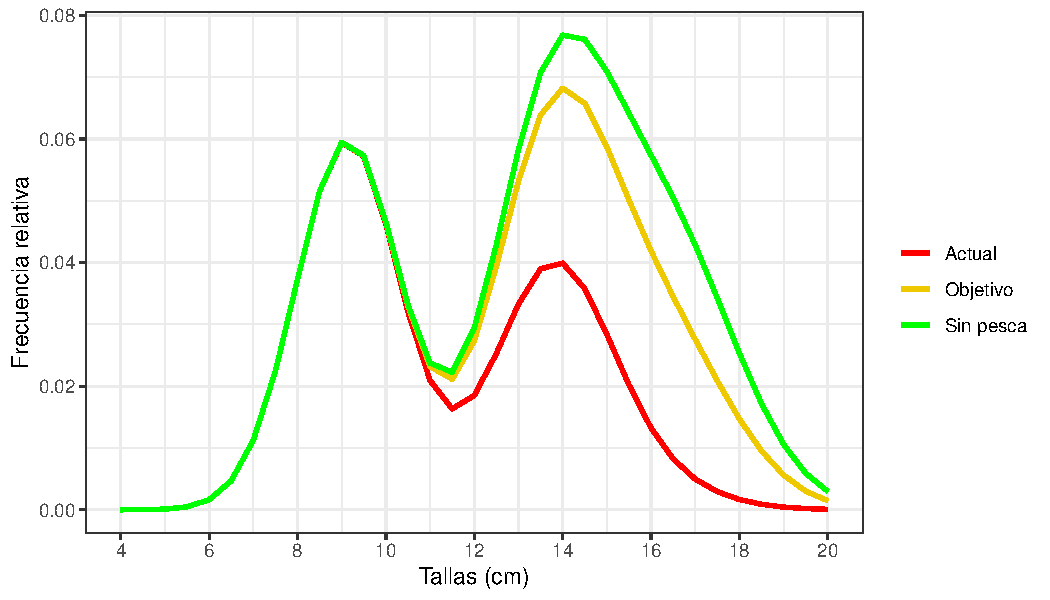
\includegraphics[width=0.7\textwidth]{LBPA/Figuras/EstatusTallas-1.pdf}
\caption{Estructuras de tallas calculadas por LBPA. La línea verde representa las tallas sin pesca, la línea amarilla muestra una estructura de talla en relación al PBR (SPR 60\%) y por ultimo la línea roja representa la talla actual.}
\label{Fig23}
\end{figure}

\begin{figure}[h!]
\centering
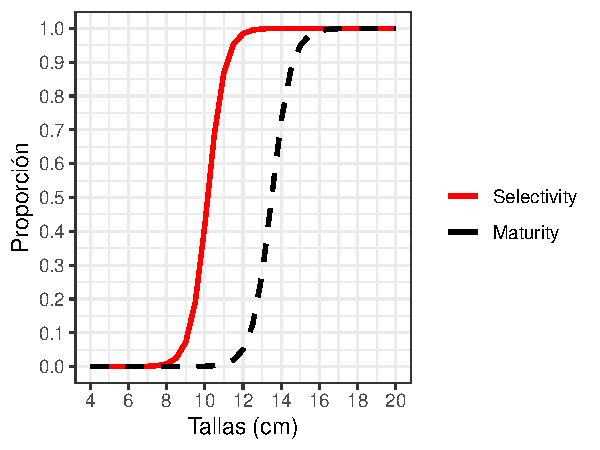
\includegraphics[width=0.7\textwidth]{LBPA/Figuras/selectividad_talla-1.pdf}
\caption{Curvas de selectividad y madurez para sardina austral de la Región de Aysén.}
\label{Fig24}
\end{figure}

\pagebreak

\begin{figure}[h!]
\centering
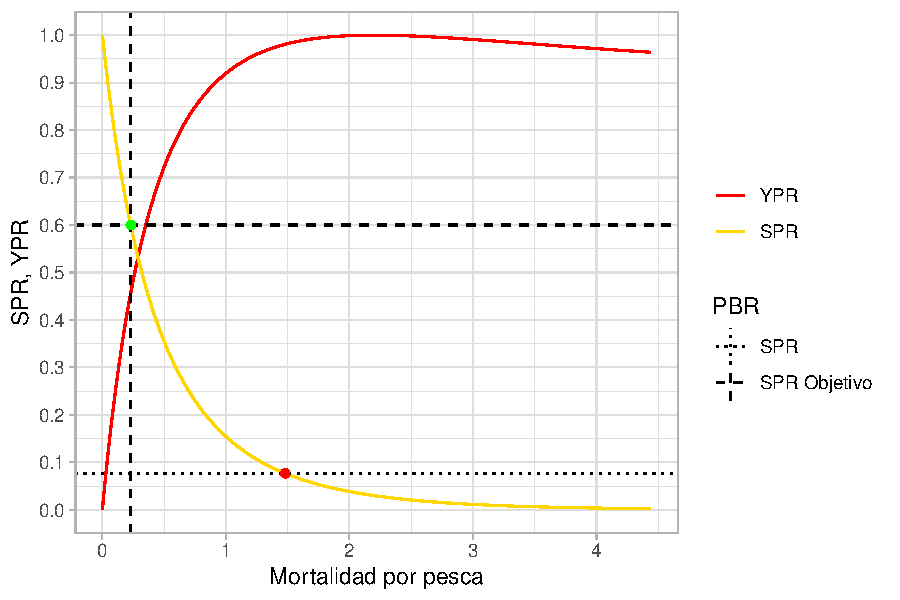
\includegraphics[width=0.7\textwidth]{LBPA/Figuras/CurvaSPR-1.pdf}
\caption{Rendimiento por Recluta y Biomasa desovante por recluta como una función de la mortalidad por pesca. En este caso el punto rojo representa el F Actual  y el punto verde el F Objetivo al SPR 60\%.}
\label{Fig25}
\end{figure}

\begin{figure}[h!]
\centering
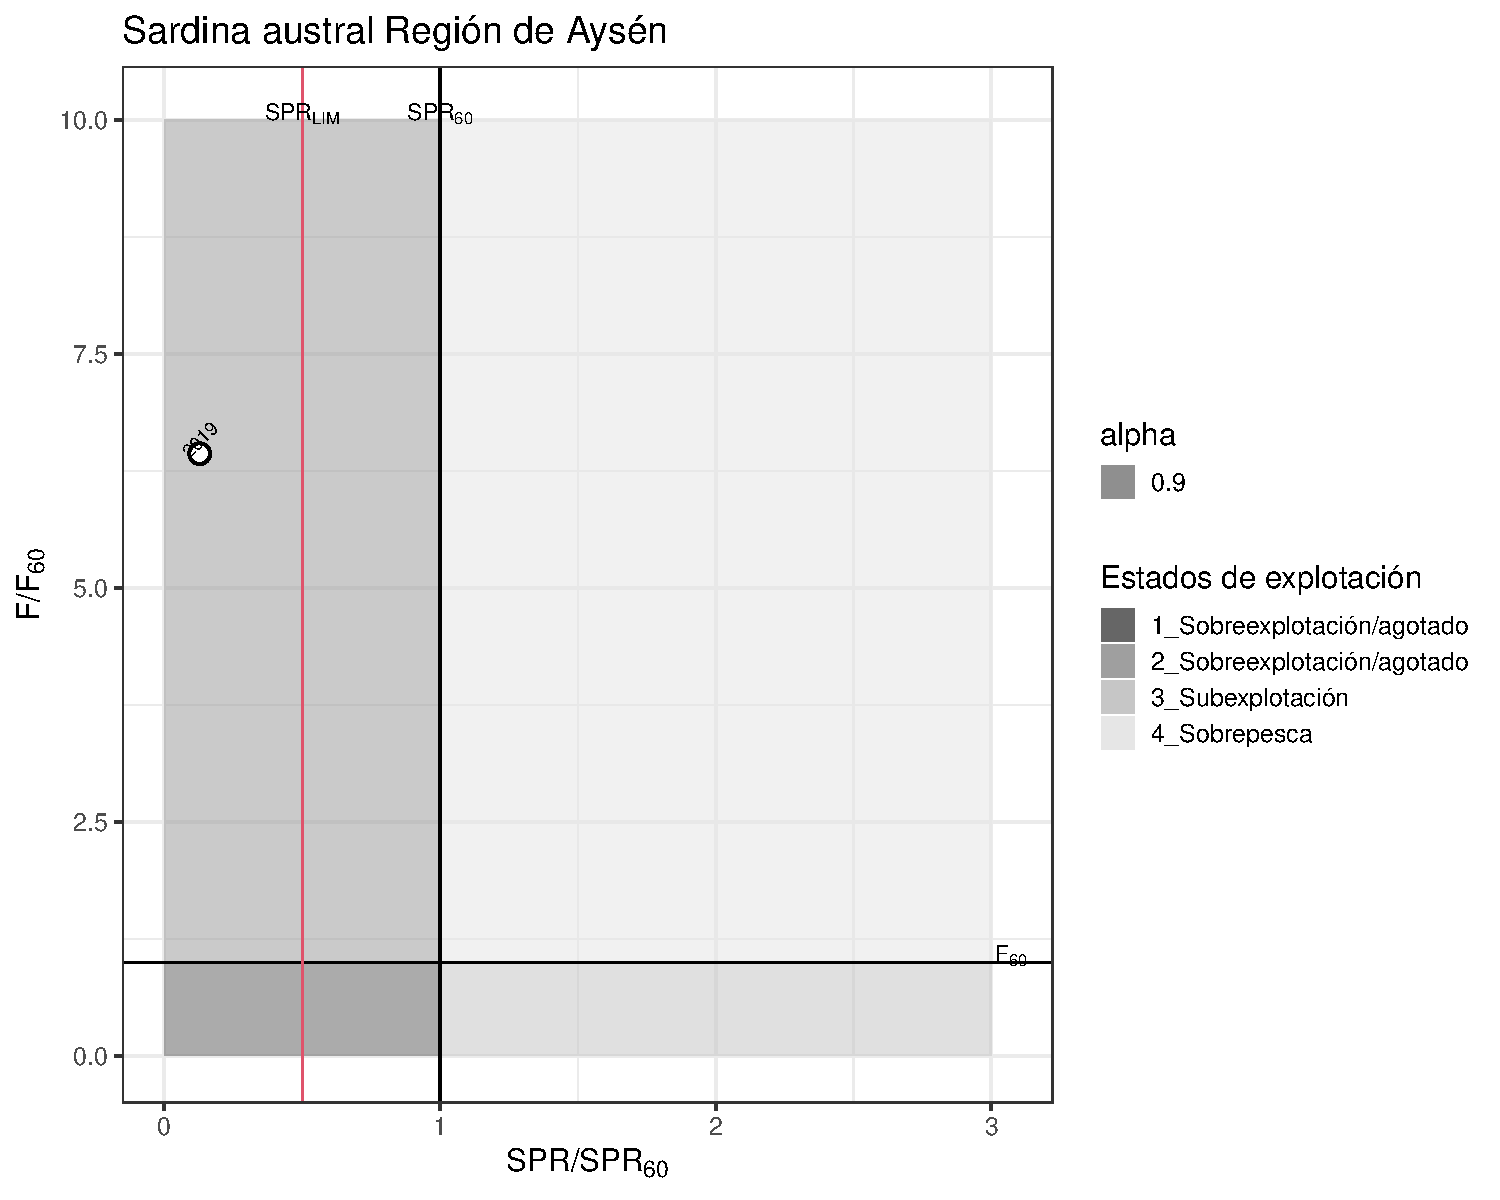
\includegraphics[width=0.7\textwidth]{LBPA/Figuras/Fig_DiagramaFaseXI-1.pdf}
\caption{Diagrama de fase de sardina austral de la Región de Aysén. Las líneas verticales segmentadas indican los PBR proxy al máximo rendimiento sostenido y aquel que indica el límite o colapso. La línea segmentada horizontal indica la mortalidad por pesca que permite el máximo rendimiento sostenido.}
\label{Fig26}
\end{figure}

\pagebreak

\hypertarget{anuxe1lisis-y-discusiuxf3n}{%
\section{5. ANÁLISIS Y DISCUSIÓN}\label{anuxe1lisis-y-discusiuxf3n}}

\hypertarget{datos-de-entrada}{%
\subsection{5.1 Datos de entrada}\label{datos-de-entrada}}

El análisis contenido en el presente informe, corresponde a la
evaluación de stock de sardina austral en la Región de Aysén hasta el
año 2020 y CBA para el año 2021. Se considera información completa de
los desembarques a diciembre de 2019 y un supesto de captura para el
2020 equivalente a cuota de captura establecida pare el año en curso.

La disminución en los indicadores poblacionales hasta el año 2018, es
coherente con la reducción en los desembarques a partir año 2015. La
misma situación se observó en el índice acústico hasta el año 2019. Esta
reducción en el índice acústico, fue similar a lo observado en la región
de Los Lagos, donde los años 2018 y 2019, se produjo un cambio de escala
en los niveles de biomasa del stock respecto de evaluaciones previas. El
año 2020 en cambio en la Región de Los Lagos se apreció un incremento
importante en este índice La biomasa acústica disminuyó desde 45 mil t
el año 2016 hasta 24,8 mil t el 2018 y 6,6 mil t en el 2019. Este último
valor fue el más bajo de toda la serie. El crucero del año 2020, no se
llevó a cabo debido a la reasignación de recursos por parte de la
Subsecretaría de Pesca para bordar otras materias de interés en esta
pesquería. Sin embargo, considerando los resultados del estudio en la
zona norte (Los Lagos), es probable que en la zona de Aysén, también se
haya manifestado un aumento en la biomasa del stock. Esto considerando
la recuperación en los desembarques durante la ultima parte del año 2019
y la primera mitad del 2020. Los años 2018 y 2019, las cifras de
desembarques oficiales de sardina austral en la Región de Aysén fueron
los mínimos de toda la serie, disminuyendo desde niveles promedio de 4,5
mil toneladas entre el 2012 y 2017 hasta 650 t el 2018 y 1,3 mil t el
2019. Se espera sin embrago, que durante el 2020 tales niveles
incrementen y alcancen valores cercanos a las 2,9 mil t.

\hypertarget{indicadores-del-stock}{%
\subsection{5.2 Indicadores del stock}\label{indicadores-del-stock}}

La biomasa estimada por el actual modelo de evaluación, se redujo
significativamente desde 16,7 mil t, el año 2012 hasta 3,5 mil t, el año
2018. La mortalidad por pesca (F) en tanto aumentó desde 0,24
año\textsuperscript{-1} al principio de la serie hasta 0.88
año\textsuperscript{-1} los años 2016 y 2017. Luego, producto de la
reducción en las remociones, la mortalidad por pesca disminuye hasta
valores por del debajo de la referencia (\(F_{RMS}\)= 0,46 año-1).

La razón \(B/B_{RMS}\), presentó una relación inversa y proporcional a
los niveles de mortalidad por pesca (F) aplicados sobre la pesquería. El
indicador, muestra una condición positiva, con valores por sobre el
objetivo Biológico de Referencia \(B_{RMS}\) hasta el 2015 y alcanza la
biomasa límite el año 2018. A partir del año 2019 muestra una
recuperación hasta 0.90 \(B_{RMS}\) el año 2020.

De acuerdo al modelo base utilizado, los resultados del análisis,
señalan que el recurso en aguas interiores de la Región de Aysén,
durante el año 2020, se encontraría por debajo del objetivo de manejo en
términos de biomasa (\(B>B_{RMS}\)), auqnue con bajos niveles de F. El
estatus del recurso, estimado a través de la metodología de Zhou
\emph{et al}., (2013), lo sitúa en límite inferior de la zona de
plena-explotación, con niveles de F por debajo de \(F_{RMS}\)
(\(F< F_{RMS}\)). Se utilizó para el presente análisis un nivel máximo
de agotamiento (D) o reducción del stock de la población de 0,5. Este
nivel de reducción corresponde a un valor diferente al utilizado en la
evaluación previa (0,4) y se justifica por la recuperación de la
actividad pesquera en la zona de análisis y los resultados del crucero
de evaluación directa en la Región de Los Lagos que mostró uno de los
niveles más altos de la serie.

A pesar que los resultados del presente análisis están fuertemente
limitados por la corta serie temporal, se considera que, además de la
pesca, posibles cambios en las condiciones el hábitat en la Regiones de
Aysén y Los Lagos, podrían haber afectado de igual manera los
reclutamientos durante los años 2017 y 2018, incidiendo en la
productividad del stock en ambas zonas.

\hypertarget{captura-bioluxf3gicamente-aceptable-cba-1}{%
\subsection{5.3 Captura Biológicamente Aceptable
(CBA)}\label{captura-bioluxf3gicamente-aceptable-cba-1}}

El rango de captura para el año 2021 para percentiles de probabilidad
entre el 10\% y 50\%, podría situarse entre 3,1 mil t y 4,2 mil t. para
niveles de mortalidad por pesca de 0,75* \(F_{RMS}\) y \(F_{RMS}\)
respectivamente. Sin embargo, considerando la condición del recurso en
los últimos años, es recomendable basarse en el enfoque precautorio y
considerar un nivel de captura más cercano al nivel inferior del rango
estimado.

\hypertarget{exploraciuxf3n-de-muxe9todos-alternativos-para-determinaciuxf3n-del-estatus}{%
\subsection{5.4. Exploración de métodos alternativos para determinación
del
estatus}\label{exploraciuxf3n-de-muxe9todos-alternativos-para-determinaciuxf3n-del-estatus}}

El Programa de Mejoramiento Continuo de la Calidad de Asesoría
Científica (PMCCAC), se enfoca en sintetizar las brechas de datos,
información y conocimiento en relación con la situación general de una
pesquería y de esta forma una sistematización para el desarrollo
continuo de la asesoría científica.

La mayoría de los métodos que se han utilizado para evaluar las
poblaciones a escala mundial son métodos de sólo captura, ya que los
datos de captura/desembarques son fáciles de obtener. Sin embargo, los
modelos basados en captura necesitan supuestos de una evaluación real, y
los datos de captura ayudan a proporcionar un contexto biológico a estos
supuestos. Al respecto, el modelo base actual utilizado para la
evaluación de stock de sardina austral de la Región de Aysén corresponde
a la aproximación de Zhou \emph{et al}. (2013), el que utiliza solo las
capturas para estimar las variables de estado como la biomasa y niveles
de mortalidad por pesca (F) que junto a los puntos biológicos de
referencia (PBRs) permiten determinar el estatus y calcular la "Captura
Biológicamente Aceptable (CBA). No obstante, este método requiere asumir
un nivel de reducción del stock para definir el estatus del recurso. Sin
estos supuestos es probable que los datos de captura se malinterpreten
por las siguientes razones: a) las capturas bajas en una serie temporal
podrían depender de diferentes factores, como la implementación de
medidas de administración, la baja demanda del mercado o el agotamiento
real de la población. b) Por el contrario, las capturas elevadas podrían
ser el resultado de un aumento del esfuerzo pesquero o de la biomasa de
la población. Como resultado, los modelos de sólo captura han intentado
integrar supuestos u otros datos para reducir su nivel de incertidumbre.
En el caso de sardina austral de Aysén se utiliza el método de Hilborn
\& Mangel (1997) que usa, además de los desembarques, un índice de
abundancia relativo, en este caso la biomasa acústica, para aproximarse
a los cambios en la pendiente de la biomasa del stock en el tiempo.

El resultado más relevante del método de Hilborn \& Mangel (1997) se
relaciona con el nivel de depleción (D) estimado para el stock, ya que
ha sido utilizado en la metodología de Zhou \emph{et al}., (2013) que es
presentado actualmente al Comité Científico de pequeños pelágicos para
definir el estatus del recurso en la Región de Aysén. En términos de
reducción, al usar toda la información disponible, los resultados
indican que, durante el 2020, el stock estaría reducido hasta un 26\% de
su condición original el año 2013. No obstante, la actividad de la flota
durante los últimos meses del 2019 y los primeros meses del 2020,
muestran una recuperación importante en sus capturas. Hasta mayo del
2020, se había desembarcado el 97\% de la cuota asignada inicialmente
para esta zona. Esto hace suponer una condición menos pesimista del
stock que el nivel de depleción (0,26) estimado por el método de Hilborn
\& Mangel (1997).

Asimismo, a pesar que el año 2020 no se realizó el estudio de evaluación
directa en la Región de Aysén, el incremento en la biomasa detectado por
el crucero en la Región de Los Lagos, hace suponer un incremento también
en el stock del sur (Aysén). Este supuesto se basa en la similitud
histórica en la variabilidad del índice acústico en ambas zonas de
evaluación. La reducción en el índice acústico el año 2019 fue similar a
lo observado en la región de Los Lagos, donde los años 2018 y 2019, se
produjo un cambio de escala en los niveles de biomasa del stock respecto
de evaluaciones previas. El año 2020 en cambio en la Región de Los Lagos
se apreció un incremento importante en este índice. De esta manera,
considerando los antecedentes previos, se utiliza en la metodología de
Zhou \emph{et al}. (2013) un nivel máximo de agotamiento (D) o reducción
del stock de la población de 0,5.

De este modo, los resultados obtenidos por el método de Zhou \emph{et
al}. (2013), muestra una condición positiva, con valores por sobre el
objetivo Biológico de Referencia \(B_{RMS}\) hasta el 2015 y alcanza la
biomasa límite el año 2018. A partir del año 2019 muestra una
recuperación hasta 0.90 \(B_{RMS}\) el año 2020. Por otro lado, la
mortalidad por pesca aumentó durante los años 2016 y 2017. Luego,
producto de la reducción en las remociones, la mortalidad por pesca
disminuye hasta valores por debajo de la referencia. El estatus estimado
durante el año 2020, se encontraría por debajo del objetivo de manejo en
términos de biomasa (\(B>B_{RMS}\)), y con bajos niveles de \(F\). A
pesar que los resultados del análisis están fuertemente limitados por la
corta serie temporal, se considera que, además de la pesca, posibles
cambios en las condiciones del hábitat en la Regiones de Aysén y Los
Lagos, podrían haber afectado de igual manera los reclutamientos durante
los años 2017 y 2018, incidiendo en la productividad del stock en ambas
zonas.

Los resultados obtenidos por el método de Zhou se consideran una
aproximación preliminar, ya que las decisiones sobre los supuestos
predeterminan el rango de valores de \(B/B_{RMS}\) que el modelo
``estima'' como estado actual. El modelo asume un modelo de Schaefer de
crecimiento de biomasa, que asume que \(B_{RMS}/K\) = 0,5. Este modelo
también requiere algunos límites en los valores \(B_{final}/K\)
plausibles (supuesto de depleción). Poniendo estos dos supuestos juntos,
encontramos que una vez que hemos decidido la relación de \(B_{RMS}/K\)
(que el modelo de Schaefer establece en 0.5), y proporcionamos límites
en el agotamiento inicial y final, hemos establecido exactamente el
rango de posibles valores inicial y final de \(B/B_{RMS}\). De este
modo, el modelo nos ayuda a interpretar nuestras suposiciones sobre el
agotamiento inicial y final en el contexto de \(B/B_{RMS}\), pero no
proporciona una nueva perspectiva de lo que puede ser \(B/B_{RMS}\) más
allá de las proporcionadas por las suposiciones realizadas. Una
respuesta natural a este problema es reflejar la incertidumbre en el
estado final del stock proporcionando una amplia gama de valores de
agotamiento para el último año de la serie. Sin embargo, dado que
siempre habrá más formas de producir niveles de agotamiento más altos
que niveles de agotamiento más bajos (ya que es más probable que los
niveles de agotamiento más bajos colapsen a la población dado el
historial de captura), ser ``conservador'' al establecer a priori el
agotamiento final necesariamente sesgará positivamente cualquier
``estimación'' final de \(B/B_{RMS}\).

Como parte del programa de mejoramiento continuo en este documento
técnico se exploran dos métodos de data poor alternativos: a) SPiCT,
Stochastic Surplus Production Model in Continuous Time (Peteresen \&
Berg, 2017), basado en datos de captura y biomasa acústica y b) LBPA,
Length-Based Pseudocohort Analysis (Canales \emph{et al}., 2021) basado
en datos de la biología (se utilizan parámetros de crecimiento, madurez
de sardina austral de la Región de Los Lagos) y pesqueros (estructura de
tallas de los años 2015 hasta el 2019) de sardina austral de la Región
de Aysén.

En relación a los modelos de producción, estos se utilizan para evaluar
biomasa y nivel de explotación de poblaciones marinas en situaciones de
datos limitados donde la información de la edad y el tamaño no están
disponibles (Punt, 2003). Estos modelos se aplican principalmente a
acciones donde los únicos datos disponibles son observaciones de
capturas comerciales junto con algún índice de biomasa explotable, como
capturas comerciales por unidad esfuerzo (CPUE), densidades medias,
estimaciones de abundancia a través de surveys o derivado de una
encuesta científica (Polacheck \emph{et al}. 1993). Aplicaciones comunes
de los modelos de producción excedente incluyen grandes peces pelágicos
migratorios como el atún, tiburones y peces picudos, pero también
crustáceos que son generalmente más longevos (por ejemplo, Smith y
Addison 2003). En la formulación de Schaefer (1954), la producción
máxima ocurre cuando el tamaño de la población es la mitad de su
capacidad de carga. Esta restricción se evita en forma generalizada al
utilizar Pella y Tomlinson (1969), donde la asimetría de la función de
producción permite la máxima producción a cualquier biomasa por debajo
de la capacidad de carga. Así, una población se explota de manera óptima
en términos de biomasa si se cosecha para permanecer en la biomasa nivel
que da como resultado la máxima producción definido como el Rendimiento
Máximo Sostenible (\(RMS\)).

En este documento técnico se presenta un modelo de producción excedente
estocástica en tiempo continuo (Stochastic Surplus Production Model in
Continuous Time, SpiCT, por sus siglas en inglés) (Pedersen \& Berg,
2017), que incorpora dinámica tanto de la biomasa como de la pesca y
error de observación tanto de las capturas como de los índices de
biomasa. El modelo tiene una forma estado-espacio que contiene error de
proceso y observación (Polacheck \emph{et al}., 1999; Polacheck \emph{et
al}. 1993; Prager, 2002), así como modelos de estado-espacio que asumen
capturas sin errores (Meyer y Millar 1999; Punt 2003; Ono \emph{et al},.
2012).

El modelo utiliza datos observados sobre desembarques o capturas e
índices, ya sean comerciales o de prospecciones y no incluye parámetros
de historia de vida. Los modelos de producción como SpiCT generalmente
funcionan mejor cuando hay mayor contraste en los datos (de esfuerzo,
biomasa, tasa de captura) (Hilborn \& Walters, 1993). Cuando la serie de
tiempo es corta o no hay contraste en los datos, es recomendable reducir
la cantidad de parámetros en el modelo para promover la estabilidad del
modelo. Para el caso de sardina austral de la Región de Aysén, no
podemos decir con certeza si la producción de biomasa está sesgada. La
capacidad de carga para el stock explotable se prevé que sea
aproximadamente 10.02 mil t. para la curva de producción general. Sin
embargo, el intervalo de dependencia es extremadamente amplio con un
intervalo más bajo de 4300 t. y un intervalo superior de 135 mil t.
Claramente, las predicciones del modelo están sufriendo debido a la
escasez de datos y quizás a una básica sintonización del modelo. Sin
embargo, el modelo proporciona una primera estimación de la abundancia
absoluta. De acuerdo al diagrama de fase estimado por el este método, la
pesquería de sardina austral estuvo sometida a bajos niveles de presión
pesquera en los primeros años analizados años, por lo cual su estado se
encuentra en niveles subexplotados. En los años recientes esta situación
cambia para pasar a una fase de sobrepesca y sobre explotación.

El segundo método alternativo analizado en este documento técnico
corresponde a un modelo de análisis de pseudocohortes basado en la
longitud (LBPA) desarrollado por Canales \emph{et. al}., (2021), en el
cual se analiza múltiples distribuciones de frecuencia de tallas de
captura simultáneamente, bajo el supuesto que refleja de mejor manera
una población en equilibrio. Algunas de las características de LBPA son
las siguientes (1) el conocimiento empírico puede incluirse como
penalizaciones en la función objetivo; (2) el modelo no está
parametrizado en términos de invariantes de historia de vida; (3) se
pueden estimar más parámetros (por ejemplo, el tamaño medio del
reclutamiento); y (4) LBPA no requiere información sobre la edad
absoluta porque la curva de crecimiento está parametrizada en términos
de un tamaño inicial, un tamaño asintótico y la tasa de crecimiento.

El método basado en talla proporciona estimaciones de la mortalidad por
pesca por talla y una aproximación del agotamiento de la población a
través de la SPR (Goodyear, 1993; Brooks \emph{et al}., 2010). La LBPA
se vuelve más robusta, cuando se analizan simultáneamente varios años de
datos de frecuencias de tallas de captura. Sin embargo, las estimaciones
de SPR son menos sensibles al número de años de datos y al tamaño de la
muestra cuando las tasas de explotación son bajas. El rendimiento mejora
más con frecuencias de tallas adicionales (independientemente de cómo se
ponderen). LBPA no estima el estado actual de una población, sino más
bien el estado durante varios años. La LBPA debe utilizarse cuando no se
dispone de series cronológicas de datos de captura o existen dudas
fundadas sobre las extracciones totales de una pesquería. El método es
particularmente útil para identificar poblaciones que están
sobreexplotadas y debe basarse en tantos años de datos de frecuencia de
tallas como sea posible. Finalmente y dependiendo de la calidad de los
datos (cantidad y contraste), la LBPA podría usarse para estimar
parámetros biológicos como los coeficientes del modelo de crecimiento o
aquellos relacionados con la variabilidad de la talla por edad. En el
caso de sardina austral de la Región de Aysén, aún existe incertidumbre
en los parámetros biológicos utilizados, ya que los antecedentes
utilizados corresponden principalmente a estimaciones realizadas a
sardina austral de la Región de Los Lagos. No obstante, las estructuras
de tallas vulneradas por la flota muestran una alta selectividad de
individuos bajo la talla de madurez de 13 cm LT y baja presencia de
individuos adultos. Esto genera una condición de sobrepesca y
sobre-explotación bajo este enfoque de modelación, misma condición
estimada por el método de producción SPICT.

Los estudios señalan que, debido a sus características reproductivas,
como baja fecundidad (Aranis \emph{et al}., 2015) y madurez a longitudes
avanzadas (Leal \emph{et al}.,2011), la sardina austral tendría un menor
potencial reproductivo en comparación a sardina común en la zona centro
sur. Esta condición, supone una mayor sensibilidad de la especie frente
a la explotación pesquera. Por lo tanto, las estrategias de explotación
deberían ser también comparativamente más cautelosas. Lo anterior
sugiere el uso de puntos biológicos de referencias (PBR) conservadores
en esta pesquería (F60\%-F65\%). Las poblaciones de peces pelágicos,
además de los factores relacionados a la explotación pesquera, están
fuertemente influenciados por factores ambientales, pudiendo presentar
amplias variaciones interanuales en su abundancia dependiendo de las
condiciones del hábitat (Bakun y Parrish, 1982; Cushing, 1990).
Asimismo, se conoce que las especies forrajeras, como sardinas y
anchovetas, cumplen un rol clave en el ecosistema marino, siendo la base
alimenticia de mamíferos, aves y peces de mayor tamaño (Pikitch \emph{et
al}., 2012). La sardina austral, en el ecosistema de fiordos del sur de
Chile, no es la excepción. Antecedentes recientes destacan a la especie,
como un componente relevante de la trama trófica marina. Neira \emph{et
al}., (2014) indican que sardina austral es presa significativa de otros
recursos pesqueros como merluza austral, merluza de cola y congrio
dorado.

\pagebreak

\hypertarget{referencias-bibliogruxe1ficas}{%
\section{6. REFERENCIAS
BIBLIOGRÁFICAS}\label{referencias-bibliogruxe1ficas}}

Aranis A., A. Gómez; L. Caballero; K. Walker; M. Ramírez; G. Eisele; F.
Cerna; C. Valero; A. López; C. Machuca; L. Muñoz; J. Letelier; C.
Toledo; V. Valdebenito y M. Albornoz. 2019. Informe Final, Programa de
Seguimiento de las principales Pesquerías Pelágicas de la Zona
Centro-Sur de Chile, 2018. Subsecretaría de Economía y EMT, Inst. Fom.
Pesq. Valparaíso, Chile

Aranis A., A. Gómez; L. Caballero; K. Walker; M. Ramírez; G. Eisele; F.
Cerna; C. Valero; A. López; C. Machuca; L. Muñoz; J. Letelier; C.
Toledo; V. Valdebenito y M. Albornoz. 2015. Informe Final, Programa de
Seguimiento de las principales Pesquerías Pelágicas de la Zona
Centro-Sur de Chile, 2017. Subsecretaría de Economía y EMT, Inst. Fom.
Pesq. Valparaíso, Chile.

Aranis A, R Meléndez, G Pequeño y F Cerna. 2007. Sprattus fuegensis en
aguas interiores de Chiloé, Chile (Osteichthyes: Clupeiformes:
Clupeidae). Gayana 71 (1): 102 -- 113.

Bakun, A. y R.H. Parrish. 1982. Turbulence, transport, and pelagic fish
in the California and Peru current systems. Rep.~Calif. coop. oceanic
Fish. Invest., 123: 99-112.

Brooks, E. N. 2002. Using reproductive values to define optimal
harvesting for multisite density-dependent populations: example with a
marine reserve. Canadian Journal of Fisheries and Aquatic Sciences,
59(5), 875--885. \url{https://doi.org/10.1139/f02-058}

Brooks, E. N., Powers, J. E., \& Cortés, E. 2010. Analytical reference
points for age-structured models: Application to data-poor fisheries.
ICES Journal of Marine Science, 67(1), 165--175.
\url{https://doi.org/10.1093/icesjms/fsp225}

Canales, C. M., Punt, A. E., \& Mardones, M. 2021. Can a length-based
pseudo-cohort analysis (LBPA) using multiple catch length-frequencies
provide insight into population status in data-poor situations?
Fisheries Research, 234(October 2020), 105810.
\url{https://doi.org/10.1016/j.fishres.2020.105810}

Cerna F, E Leal, A López y G Plaza. 2013. Age, growth and natural
mortality of the Patagonian sprat Sprattus fuegensis (Jenyns, 1842) in
Chiloé inland sea, southern Chile. Latin American Journal of Aquatic
Research. 42(3): 580-587.

Cerna F, J Quiroz, A López y A Aranis. 2007. Edad y Crecimiento de
sardina fueguina (\emph{Sprattus fueguensis}, Jenyns, 1842) en el Mar
Interior de la Isla Chiloé, Pacifico Sur-Este frente a Chile. XXVII
Jornadas Ciencias del Mar.~Iquique - Chile.

Chen, Y. \& N. Andrew. 1998. Parameter Estimation in modelling the
dynamics of fish stock biomass: Is currently used observation-error
estimator reliable? Canadian Journal of Fishery and Aquatic Sciences 55:
749-760.

Cushing, D.H. 1990. Plankton production and yearclass strength in fish
populations: an update of the match/mismatch hypothesis. Adv.
Mar.~Biol., 26: 249-293.

Ernst B, J Valero y O Hamel. 2015. Programa anual de revisión experta a
la asesoría científica de las principales pesquerías nacionales, año
2013: sardina austral (\emph{Sprattus fuegensis}). Informe Final.
Proyecto N° 2013-125-FAP-20. 176 pp.

FAO. 1996. Orientaciones técnicas para la pesca responsible. N°2.
Enfoque precautorio para la pesca de captura y la introducción de
especies. Organización de las naciones unidas para la agricultura y la
alimentación. Roma. 64 pp.

Galleguillos R, S Ferrada, C Canales, C Hernández, M Oliva, MT González,
L Cubillos, E Niklitschek y P Toledo. 2012. ``Determinación de unidades
poblacionales de sardina austral entre la X y XII Regiónes de Chile'':
Proyecto FIP 2010-17. Informe Final. 171 pp.

Goodyear, C. P. (1993). Spawning stock biomass per recruit in fisheries
management: foundation and current use. Risk Evaluation and Biological
Reference Points for Fisheries Management, 120, 67--81.

Haddon M. 2001. Modelling and quantitative methods in fisheries, 406
pp.~Chapman and Hall, Boca Ratón.

Hilborn, R. \& M. Mangel. 1997. The Ecological Detective: Confronting
Models With Data. Princeton University Press, Princeton, New Jersey,
USA.

Leal E, C Canales, MJ Zúñiga y D Bucarey. 2018. Estatus y posibilidades
de explotación biológicamente sustentables de los principales recursos
pesqueros nacionales 2019: Sardina austral Región de Los Lagos. Primer
Informe (septiembre 2018). Convenio de Desempeño Subsecretaría de
Economía y EMT / IFOP, Chile: 60 pág. + Anexos.

Leal E, TM Canales, A Aranis y M González. 2011. Actividad reproductiva
y longitud de madurez de sardina austral \emph{Sprattus fuegensis}, en
el mar interior de Chiloé, Chile. Revista de Biología Marina y
Oceanografía. 46 (1): 43-51.

Neira S, H Arancibia, M Barros, L Castro, L Cubillos, E Niklitschek y R
Alarcón. 2014. Rol ecosistémico de sardina austral e impacto de su
explotación en la sustentabilidad de otras especies de interés
comercial. Pre-Informe Final Proyecto FIP 2012-15 (mayo). Universidad de
Concepción, 220 págs.

Payá I, C Canales, D Bucarey, M Canales, F Contreras, F Espíndola, E
Leal, C Montenegro, J Quiroz y R. Tascheri. 2014. Revisión de los puntos
biológicos de referencia (Rendimiento Máximo Sostenible) en las
pesquerías nacionales." Primer Taller internacional. Informe de Avance
1. Subsecretaría de Economía - IFOP. 32 pp.+ 4 Anexos.

Pedersen, M. W., \& Berg, C. W. 2017. A stochastic surplus production
model in continuous time. Fish and Fisheries, 18(2), 226--243.
\url{https://doi.org/10.1111/faf.12174}

Pella, J.J. and Tomlinson, P.K. 1969. A generalized stock production
model. Bulletin of the Inter-American Tropical Tuna Commission 13,
421--458.

Pikitch E., P. Boersma, I. Boyd, O. Conover, P. Cury, T. Essington, S.
Heppell, E. Houde, M. Mangel, D. Pauly, E. Plagányi, K. Sainsbury y R.
Steneck. 2012. Little Fish, Big Impact: Managing a Crucial Link in Ocean
Food Webs. Lenfest Ocean Program. Washington, DC. 108 pp.

Polacheck, T., Klaer, N. L., Millar, C., \& Preece, A. L. 1999. An
initial evaluation of management strategies for the southern bluefin
tuna fishery. 811--826.

Prager, M. H. (2002). Comparison of logistic and generalized
surplus-production models applied to swordfish , \emph{Xiphias gladius}
, in the north Atlantic Ocean. 58, 41--57.

Punt, A. E. 2003. The performance of a size-structured stock assessment
method in the face of spatial heterogeneity in growth. Fisheries
Research, 65(1--3), 391--409.
\url{https://doi.org/10.1016/j.fishres.2003.09.028}

Schaefer M. 1954. Some aspects of the dynamics of populations important
to the management of the commercial marine fisheries. Bull Inter-Amer.
Trop. Tuna Comm. (I-ATTC)/Bol. CIAT, 1(2): 27-56.

Vega R, L Ossa, B Suaréz,MF Jimenez, S Henríquez \& A Gonzalez. 2020.
Resultados del programa de investigación y propuestas de medidas de
mitigación del descarte y la captura incidental para la Pesquería
artesanal de sardina austral de la Región de Los Lagos. Convenio de
desempeño 2019 -- IFOP/Subsecretaría de economía y EMT-- Documento
técnico. 83 pp + Anexos.

Williams, E. \& M. Prager. 2002. Comparison of equilibrium and
nonequilibrium estimators for the generalized production model. Canadian
Journal of Fishery and Aquatic Sciences 59:1533-1552.

Zhou S, S Pascoe, N Dowling, M Haddon, N Klaer, J Larcombe, M Smith, O
Thebaud, S Vieira \& S Wayte. (2013). Quantitatively defining biological
and economic reference points in data poor and data limited fisheries.
Final Report on FRDC Project 2010/044. Canberra, Australia.

Zhou S, S Yin, T Thorson, M Smith \& M Fuller. 2012. Linking fishing
mortality reference points to life history traits: an empirical study.
Canadian Journal of Fisheries and Aquatic Science, 69: 1292-1301

\end{document}
